\documentclass[10pt,letterpaper,cm]{nupset}
\usepackage[margin=1.2in]{geometry}
\usepackage{graphicx}
 \usepackage{enumerate}
  \usepackage{enumitem}
 \usepackage{stmaryrd}
 \usepackage{bm}
\usepackage{amsfonts}
\usepackage{amssymb}
\usepackage{pgfplots}
\pgfplotsset{compat=1.13}
\usepackage{amsmath,amsthm}
\usepackage{lmodern}
\usepackage{tikz-cd}
\usetikzlibrary{quotes}
\usetikzlibrary{decorations.markings}
\usepackage{faktor}
\usepackage{xcolor}
\usepackage{soul}
\usepackage{xfrac}
\usepackage{mathtools}
\usepackage{bm}
\usepackage{ dsfont }
\usepackage{mathrsfs}
\usepackage{hyperref}
\usepackage{siunitx}
\usepackage[utf8]{inputenc}
\sisetup{group-separator={,}}
\hypersetup{colorlinks=true, linkcolor=red,          % color of internal links (change box color with linkbordercolor)
    citecolor=green,        % color of links to bibliography
    filecolor=magenta,      % color of file links
    urlcolor=cyan           }

\usepackage{thmtools}
\usepackage[capitalise]{cleveref} 
    
\theoremstyle{definition}
\newtheorem{definition}{Definition}[subsection]
\newtheorem{exmp}[definition]{Example}
\newtheorem{non-exmp}[definition]{Non-example}
\newtheorem{note}[definition]{Note}

\theoremstyle{theorem}
\newtheorem{theorem}[definition]{Theorem}
\newtheorem{lemma}[definition]{Lemma}
\newtheorem{prop}[definition]{Proposition}
\newtheorem{corollary}[definition]{Corollary}
\newtheorem*{claim}{Claim}
\newtheorem{exercise}[definition]{Exercise}

\theoremstyle{remark}
\newtheorem{remark}[definition]{Remark}
\newtheorem*{todo}{To do}
\newtheorem*{question}{Question}
\newtheorem*{conv}{Convention}
\newtheorem*{aside}{Aside}
\newtheorem*{notation}{Notation}
\newtheorem*{term}{Terminology}
\newtheorem*{background}{Background}
\newtheorem*{further}{Further reading}
\newtheorem*{sources}{Sources}

\makeatletter
\def\th@plain{%
  \thm@notefont{}% same as heading font
  \itshape % body font
}
\def\th@definition{%
  \thm@notefont{}% same as heading font
  \normalfont % body font
}
\makeatother

\makeatletter
\renewcommand*\env@matrix[1][*\c@MaxMatrixCols c]{%
  \hskip -\arraycolsep
  \let\@ifnextchar\new@ifnextchar
  \array{#1}}
\makeatother
\pgfplotsset{unit circle/.style={width=4cm,height=4cm,axis lines=middle,xtick=\empty,ytick=\empty,axis equal,enlargelimits,xmax=1,ymax=1,xmin=-1,ymin=-1,domain=0:pi/2}}
\DeclareMathOperator{\Ima}{Im}
\newcommand{\A}{\mathcal A}
\newcommand{\C}{\mathbb C}
\newcommand{\D}{\mathcal{D}}
\newcommand{\E}{\vec E}
\newcommand{\CP}{\mathbb CP}
\newcommand{\F}{\mathbb F}
\newcommand{\G}{\mathbb G}
\renewcommand{\H}{\mathbb H}
\newcommand{\HP}{\mathbb HP}
\newcommand{\K}{\mathbb K}
\renewcommand{\L}{\mathcal L}
\newcommand{\M}{\mathbb M}
\newcommand{\N}{\mathbb N}
\renewcommand{\O}{\mathbf O}
\newcommand{\OP}{\mathbb OP}
\renewcommand{\P}{\mathcal P}
\newcommand{\Q}{\mathbb Q}
\newcommand{\I}{\mathbb I}
\newcommand{\R}{\mathbb R}
\newcommand{\RP}{\mathbb RP}
\renewcommand{\S}{\mathbf S}
\newcommand{\T}{\mathbf T}
\newcommand{\Z}{\mathbb Z}
\newcommand{\B}{\mathcal{B}}
\newcommand{\1}{\mathbf{1}}
\newcommand{\ds}{\displaystyle}
\newcommand{\ran}{\right>}
\newcommand{\lan}{\left<}
\newcommand{\bmat}[1]{\begin{bmatrix} #1 \end{bmatrix}}

\renewcommand{\a}{\mathscr{A}}
\renewcommand{\b}{\mathscr{B}}
\renewcommand{\c}{\mathscr{C}}
\renewcommand{\d}{\mathscr{D}}
\newcommand{\e}{\mathscr{E}}
\newcommand{\y}{\mathscr{Y}}
\renewcommand{\j}{\mathscr{J}}
\newcommand{\X}{\mathscr X}

\newcommand{\h}{\vec h}
\newcommand{\f}{\vec f}
\newcommand{\g}{\vec g}
\renewcommand{\i}{\mathscr{I}}
\renewcommand{\k}{\vec k}
\newcommand{\n}{\vec n}
\newcommand{\p}{\frak{p}}
\newcommand{\q}{\mathscr{Q}}
\renewcommand{\r}{\vec r}
\newcommand{\s}{\vec s}
\renewcommand{\t}{\vec t}
\renewcommand{\u}{\mathscr{U}}
\renewcommand{\v}{\mathscr{V}}
\newcommand{\w}{\vec w}
\newcommand{\x}{\vec x}
\newcommand{\z}{\vec z}
\newcommand{\0}{\vec 0}

\newcommand{\arrowcircle}[1][]{%
  \begin{tikzpicture}[#1]
    \draw[->] (0,0ex) -- (2em,0ex);
    \draw (1em,0ex) circle (0.7ex);
  \end{tikzpicture}%
}

\DeclareMathOperator{\card}{\text{card}}

\newcommand{\Rho}{\mathrm{P}}

\newcommand{\properideal}{%
  \mathrel{\ooalign{$\lneq$\cr\raise.22ex\hbox{$\lhd$}\cr}}}

\makeatletter
\newcommand*\bigcdot{\mathpalette\bigcdot@{.5}}
\newcommand*\bigcdot@[2]{\mathbin{\vcenter{\hbox{\scalebox{#2}{$\m@th#1\bullet$}}}}}
\makeatother

\DeclareMathOperator*{\Span}{span}
\DeclareMathOperator{\lcm}{lcm}
\DeclareMathOperator*{\GL}{GL}
\DeclareMathOperator*{\SL}{SL}
\DeclareMathOperator{\rng}{range}
\DeclareMathOperator{\gemu}{gemu}
\DeclareMathOperator{\almu}{almu}
\DeclareMathOperator{\ann}{ann}
\DeclareMathOperator{\Char}{\mathsf{char}}
\DeclareMathOperator{\id}{id}
\DeclareMathOperator{\graph}{Graph}
\DeclareMathOperator{\gal}{Gal}
\DeclareMathOperator{\tr}{tr}
\DeclareMathOperator{\trdeg}{trdeg}
\DeclareMathOperator{\ev}{ev}
\DeclareMathOperator{\norm}{N}
\DeclareMathOperator{\aut}{Aut}
\DeclareMathOperator{\Int}{Int}
\DeclareMathOperator{\ext}{Ext}
\DeclareMathOperator{\stab}{Stab}
\DeclareMathOperator{\orb}{Orb}
\DeclareMathOperator{\inn}{Inn}
\DeclareMathOperator{\out}{Out}
\DeclareMathOperator{\op}{op}
\DeclareMathOperator{\fix}{Fix}
\DeclareMathOperator{\ab}{ab}
\DeclareMathOperator{\sgn}{sgn}
\DeclareMathOperator{\syl}{syl}
\DeclareMathOperator{\Syl}{Syl}
\DeclareMathOperator{\conj}{conj}
\DeclareMathOperator{\im}{im}
\DeclareMathOperator{\ed}{End}
\DeclareMathOperator{\gr}{\mathsf{gr}}
\DeclareMathOperator{\map}{Map}
\DeclareMathOperator{\mor}{mor}
\DeclareMathOperator{\ob}{ob}
\DeclareMathOperator{\pr}{pr}
\DeclareMathOperator{\fs}{fs}
\DeclareMathOperator{\cl}{cl}
\DeclareMathOperator{\Sing}{Sing}
\DeclareMathOperator{\Mat}{Mat}
\DeclareMathOperator{\Hom}{Hom}
\DeclareMathOperator{\Fun}{Fun}
\DeclareMathOperator{\Fr}{Fr}
\DeclareMathOperator{\cone}{cone}
\DeclareMathOperator{\colim}{colim}
\DeclareMathOperator{\nilp}{Nilp}
\DeclareMathOperator{\tot}{Tot}
\DeclareMathOperator{\kor}{Kor}
\DeclareMathOperator{\Jac}{Jac}
\DeclareMathOperator{\Max}{Max}
\DeclareMathOperator{\ho}{Ho}
\DeclareMathOperator{\mult}{mult}
\DeclareMathOperator{\Frac}{Frac}
\DeclareMathOperator{\disc}{Discr}
\DeclareMathOperator{\supp}{supp}
\DeclareMathOperator{\acyc}{acyclic}

\pagestyle{headings}

\linespread{1.3}

% info for header block in upper right hand corner
\name{Perry Hart}
\class{MATH 603}
\assignment{Spring 2019}

\begin{document}
\thispagestyle{empty}
\begin{abstract}
These notes are based on Tony Pantev's ``Algebra II'' lectures at UPenn. Any mistake in what follows is my own.
\end{abstract}

\tableofcontents
\newpage

\section{Injective and flat modules}

\subsection{Lecture 1}

\begin{prop} An $R$-module $M$ is injective if and only if we can fill any injectivity diagram of ideal type, i.e.,  

\[
\begin{tikzcd}
 &  & M \\
0 \arrow[r] & \frak{a} \arrow[r] \arrow[ru] & R \arrow[u, dashed]
\end{tikzcd}
\] 
where $\frak{a}$ is an ideal in $R$.
\end{prop}
\begin{proof} $ $
\smallskip

$(\Longrightarrow)$

This is obvious.

\medskip


$(\Longleftarrow)$ 

Let 
\[
\begin{tikzcd}
 &  & M \\
0 \arrow[r] & X' \arrow[ru, "\varphi"] \arrow[r] & X
\end{tikzcd} \] 
be an injectivity diagram of $R$-modules and define $$S = \left\{(A, \xi) \mid X' \subset A \subset X, \ \xi : A \to M, \ \xi \restriction_{X'} = \varphi\right\} . $$ By Zorn's lemma, there is some maximal element $(N, \psi)$ of $S$. Suppose, toward a contradiction, that $X \ne N$. Pick any $x\in X \setminus N$. We have the ideal $$\frak{a} \coloneqq  \left\{a \in R : ax \in N\right\}$$ in $R$. Define the $R$-module morphism $\theta : \frak{a} \to M$ by $a \mapsto \psi(ax)$. By hypothesis, we get the following commutative diagram.
\[
\begin{tikzcd}
 &  & M \\
0 \arrow[r] & \frak{a} \arrow[ru, "\theta"] \arrow[r, hook] & R \arrow[u, "\tilde{\theta}"', dashed]
\end{tikzcd}
\] Define the $R$-submodule $\widetilde{N} = \langle N, x\rangle$. We can write any $z\in \widetilde{N}$ as $z = y + ax$ for some $y\in N$ and some $a\in R$. Define $\tilde{\psi} : \widetilde{N} \to M$ by $y+ax \mapsto \psi(y) + \tilde{\theta}(a)$. To see that this is well-defined, let $y+ax = y'+a'x$. Then $(y-y') = (a'-a)x$, so that $$\psi(y-y') = \psi((a'-a)x) = \tilde{\theta}(a'-a) = \tilde{\theta}(a') - \tilde{\theta}(a) . $$
This implies that $\tilde{\psi}$ is a well-defined homomorphism. But then $\left(\widetilde{N}, \tilde{\psi}\right)> \left(N, \psi\right)$, a contradiction.  
\end{proof}

\begin{aside}
The categorical dual $\Rho^{\op}$ of this recognition principle for injectivity expresses a recognition principle for projectivity, namely that for any $R$-module $M$, ideal $I\subset R$, and homomorphism $\varphi : M \to \faktor{R}{I}$, we can fill the diagram
\[ \tag{$\ast$}
\begin{tikzcd}
M \arrow[rd, "\varphi"] \arrow[d, dashed] &  &  \\
R \arrow[r, two heads] & \faktor{R}{I} \arrow[r] & 0
\end{tikzcd}
\] if and only if $M$ is projective. This is equivalent to saying that $M$ is projective if and only if the natural group map $\Hom_R(M, R) \to \Hom_R \left(M, \faktor{R}{I} \right)$ is surjective. 
But then $\Rho^{\op}$ is precisely an affirmative answer to what is known as ``Faith's problem on $R$-projectivity,'' which Trlifaj (2017) proved to be undecidable in ZFC + GCH. Therefore, both $\Rho^{\op}$ and $\neg (\Rho^{\op})$ are consistent with ZFC + GCH.
\end{aside}

\begin{corollary} $ $
\begin{enumerate}
\item If $R$ is an integral domain, then any injective $R$-module $M$ is divisible.
\item If $R$ is a PID, then $M$ is injective if and only if it is divisible.
\end{enumerate}
\end{corollary}
\begin{proof} $ $
\begin{enumerate}
\item Given any $a\in R$, we want to show that the homomorphism $\mult_a : M \to M$ given by $x\mapsto ax$ is surjective. The assumption that $R$ is an integral domain entails that $\mult_a : R\to R$ is injective. Note that $\frak{a}\coloneqq  \mult_a(R)$ is an ideal in $R$, giving the short exact sequence $$0 \to \frak{a} \to R \to \faktor{R}{\frak{a}}\to 0.  $$ By assumption, $\Hom_R(-, M)$ is exact, so that the sequence $$0 \to \Hom\left(\faktor{R}{\frak{a}}, M \right) \to \Hom_R(R, M) \to \Hom_R(\frak{a}, M) \to 0   $$ is exact. Since $R$ and $\frak{a}$ are free $R$-modules of rank $1$, it follows that $\Hom_R(R, M) \cong M \cong  \Hom_R(\frak{a}, M)$. This means that the sequence  $$0 \to \Hom\left(\faktor{R}{\frak{a}}, M \right) \to M \overset{\mult_a}{\longrightarrow} M \to 0 $$ exact. In particular $\mult_a$ is surjective.

\item $(\Longleftarrow)$ Suppose that $M$ is divisible and $R$ is a PID. We want to fill the injectivity diagram
\[
\begin{tikzcd}
 &  & M \\
0 \arrow[r] & \frak{a} \arrow[r] \arrow[ru, "\varphi"] & R \arrow[u, "\psi", dashed]
\end{tikzcd}.
\]
where $\frak{a}$ is an ideal in $R$. We have that $\frak{a} = (a)$. Therefore, the short exact sequence $$0 \to \frak{a} \to R \to \faktor{R}{\frak{a}} \to 0$$ is isomorphic to $0 \to R \overset{\mult_a}{\longrightarrow} R \to \faktor{R}{\frak{a}}\to 0$. Since $M$ is divisible, we know that $M \overset{\mult_a}{\longrightarrow} M \to 0$ is exact.  Apply $\Hom_R(-, M)$ to get the sequence $$\Hom_R(R, M) \overset{(-)\circ \mult_a}{\longrightarrow} \Hom_R(R, M) \to 0,$$ which is isomorphic $M \overset{\mult_a}{\longrightarrow} M \to 0$. This shows that $\Hom_R(R, M) \overset{(-)\circ \mult_a}{\longrightarrow} \Hom_R(R, M)$ is surjective. It follows that $\varphi$ can be lifted to some $\psi : R \to M$.
\end{enumerate}
\end{proof}

\subsection{Lecture 2}

\begin{corollary}
Any abelian group is injective if and only if it's divisible. 
\end{corollary}

\begin{corollary}
If $R$ is a PID and $M$ is an injective $R$-module, then every quotient of $M$ is injective.
\end{corollary}
\begin{proof}
This follows from the fact that any quotient of a divisible group is divisible.
\end{proof}

\begin{exmp} $ $
\begin{enumerate}
\item $\faktor{\Q}{\Z}$ is injective.
\item $S^1$ is injective.
\item Any non-trivial finitely generated abelian group $G$ is never injective.
\begin{proof}
It suffices to show that $G$ is never divisible. There exists a maximal proper subgroup $H\leq G$. Then $\faktor{G}{H}$ is a simple abelian group, so that $\faktor{G}{H} \cong C_p$ for some prime $p$. If $G$ is divisible, then so must $\faktor{G}{H}$. But $C_p$ is not divisible, a contradiction. 
\end{proof}
\end{enumerate}
\end{exmp}

\begin{theorem}[Baer embedding]
If $R$ is a ring, then every module embeds into an injective module.
\begin{corollary}
For any $R$-module $M$, we can find an injective resolution $$ 0 \to M \to I_0 \to I_1 \to \cdots \to I_k \to \cdots  . $$
\end{corollary} 
\end{theorem}
\begin{proof}
We want to invent a duality operation that will convert $R {-} \mathbf{Mod}^{\op}$ to  $R^{\op} {-} \mathbf{Mod}$ and then use projective objects in $R^{\op}{-}\mathbf{Mod}$. If $T$ is an abelian group, then the functor $$ \mathbf{Ab}\underset{\Hom_{\mathbf{Ab}}(-, T)}{ \longrightarrow} \mathbf{Ab}^{\op}$$ will reverse arrows. The choice of $T$ that ends up working is precisely $\faktor{\Q}{\Z}$.
\begin{claim}
Let $\Hom_{\mathbf{Ab}}(-, \faktor{\Q}{\Z}) \coloneqq  (-)^D$. Note that for any abelian group $A$, we have a canonical homomorphism $\epsilon_A : A \to A^{DD}$ given by $a \mapsto \left(\left[\varphi :A \to \faktor{\Q}{\Z}\right] \to \varphi(a)\right).$ Then $\epsilon_A$ is injective.
\end{claim}
\begin{proof}
We need to show that if $a\in A$ is nonzero, then we can find some homomorphism $f: A \to \faktor{\Q}{\Z}$ such that $f(a) \ne 0$.

\underline{Case 1:} Suppose that $\left\lvert{(a)}\right\rvert = n< \infty$. Then define the homomorphism $\varphi : (a) \to \faktor{\Q}{\Z}$ by $a \mapsto [\frac{1}{n}]$. Since $\faktor{\Q}{\Z}$ is divisible in $\mathbf{Ab}$, it is also injective. Thus, we may find some map  $\psi$ such that 
\[
\begin{tikzcd}
 &  & \faktor{\Q}{\Z} \\
0 \arrow[r] & (a) \arrow[r, hook] \arrow[ru, "\varphi"] & A \arrow[u, "\psi"', dashed]
\end{tikzcd}
\] commutes. This means that $\psi(a) \ne 0$, as required.

\underline{Case 2:} If $(a)$ has infinite order, then define $\varphi : (a) \to \faktor{\Q}{\Z}$ by $a \mapsto \frac{1}{2}$ and apply a similar argument to Case 1.
\end{proof}


The duality functor $(-)^D$ extends to a functor $ (-)^D: R^{\op}{-}\mathbf{Mod} \to R {-}\mathbf{Mod}^{\op}$ that is compatible with forgetting the module structure. Indeed, if $M$ is a left module over $R^{\op}$, then its module structure is given by a collection of maps $\left\{\mult_a : M \to M \mid a\in R\right\}$. Note that $$ \mult_a \circ \mult_b = \mult_{a \cdot_{R^{\op}} b} =  \mult_{b \cdot_{R} a}   .$$ For each $a\in R$, let $\underline{\mult}_a(\varphi) = \varphi \circ {\mult}_a$. Then the abelian group $M^D$ has an $R$-module structure given by $ \underline{\mult}_a: M^D \to M^D$, which clearly satisfies $$\underline{\mult}_{ab} = \underline{\mult}_a \circ\underline{\mult}_b.$$


\begin{lemma}\label{l1}
If $M$ is a projective $R^{\op}$-module, then $M^D$ is an injective $R$-module.
\end{lemma}
\begin{proof}
Suppose that $M$ is a projective $R^{\op}$-module and consider the injectivity diagram 
\[
\begin{tikzcd}
 &  & M^D \\
0 \arrow[r] & X' \arrow[r] \arrow[ru, "\varphi"] & X
\end{tikzcd}
\] of $R$-modules. We want to lift $\varphi : X' \to M^D$ to a map $\psi : X \to M^D$.  Apply $(-)^D$ to get a commutative diagram
\[
\begin{tikzcd}
 &  & M^{DD} \arrow[ld, "\varphi^D"'] \\
0 & (X')^D \arrow[l] & X^D \arrow[l]
\end{tikzcd}
\]
where the bottom row is exact because $\faktor{\Q}{\Z}$ is injective. 
\begin{exercise}                                                                                                  
Show that $\epsilon_M: M \to M^{DD}$ is a map of $R^{\op}$-modules.                                               
\end{exercise}   
We now have the following projectivity diagram of $R^{\op}$-modules.
\[
\begin{tikzcd}
M \arrow[rd, "\epsilon_M \circ \varphi^D"] &  &  \\
X^D \arrow[r] & (X')^D \arrow[r] & 0
\end{tikzcd}
\]
By assumption, we may fill this diagram with some map $\psi : M \to X^D$. This induces the map $\psi^D : X^{DD} \to M^D$. Note that $(\epsilon_M)^D \circ \varphi^{DD} = \psi^D \circ i^{DD}$ where $i : X' \hookrightarrow X$. But $i^{DD}\restriction_{X'} =i$ and $\varphi^{DD}\restriction_{X'} = \varphi$, so that $$\psi^D \circ i = (\epsilon_M)^D \circ  \varphi = \varphi$$ on $X'$. It follows that
\[
\begin{tikzcd}
 &  & M^D \\
0 \arrow[r] & X' \arrow[r] \arrow[ru, "\varphi"] & X \arrow[u, "\psi^D \circ \epsilon_X"']
\end{tikzcd}
\] commutes.
\end{proof}
There is some surjection $\bigoplus_{j\in J} R \to M^D$. Therefore, we have a sequence of embeddings $$M \hookrightarrow M^{DD} =\Hom_{\Z}\left(M^D, \faktor{\Q}{\Z} \right) \hookrightarrow \Hom_{\Z}\left(\bigoplus_{j\in J} R, \faktor{\Q}{\Z}\right) = \underbrace{\left(\bigoplus_{j\in J} R \right)^D}_{\text{injective by \cref{l1}}}.$$
\end{proof}

\begin{definition}
Given two $R$-modules $M$ and $N$, the \textit{additive invariants of $M$ and $N$} are the abelian groups $$\ext^i_R (M, N): = H^i(\Hom_R(P^{\bullet}, N))$$ indexed by $\N$  where $P^{\bullet}$ is a chosen projective resolution of $M$. 
\end{definition}

\begin{prop}\label{prop2} $ $
\begin{enumerate}
\item $\ext^i_R(M, N)$ is independent of our choice of projective resolution. 
\begin{proof}
This follows from the fact that any two projective resolutions are chain homotopic.
\end{proof}
\item $\ext^i_R(M, N) = H^i(\Hom_R(M, I_{\bullet}))$ for any injective resolution $I_{\bullet}$ of $N$.
\end{enumerate}
\end{prop}

\begin{lemma} $ $
\begin{enumerate}
\item $\ext^0_R(M, N) = \Hom_R(M, N)$
\item $\ext^1_R(M, N) = \left( \text{the group of isomorphism classes of extensions of } N \text{ by } M\text{ in } R{-}\mathbf{Mod}    \right)$.
\end{enumerate}                                                                                                \end{lemma}
\begin{proof}
Let $$\cdots \overset{\partial_1}{\longrightarrow} P^1 \overset{\partial_0}{\longrightarrow} P^0  \overset{\epsilon}{\longrightarrow} M \to 0$$ be a projective resolution and
let $$(\xi) : 0 \to N \overset{f}{\longrightarrow} T \overset{g}{\longrightarrow} M \to 0$$ be a short exact sequence of $R$-modules.
Note that $\Hom_R(P^k, -)$ is exact for each $k\geq 0$. Therefore, the sequence $$ 0 \to \Hom_R(P^k, N) \overset{f_k}{\longrightarrow} \Hom_R(P^k, T) \overset{g_k}{\longrightarrow} \Hom_R(P^k, M) \to 0   $$ is exact where $f_k \coloneqq  f\circ (-)$ and $g_k \coloneqq  g \circ (-)$. Letting $d_i \coloneqq  (-)\circ \partial_i$, we get \textit{short exact sequences of complexes} constituting the columns of 
\[
\begin{tikzcd}
0 \arrow[r] & {\Hom_R(P^0, N)} \arrow[r, "f_0"] \arrow[d, "d_0"] & {\Hom_R(P^0, T)} \arrow[r, "g_0"] \arrow[d, "d_0"] & {\Hom_R(P^0, M)} \arrow[r] \arrow[d, "d_0"] & 0 \\
0 \arrow[r] & {\Hom_R(P^1, N)} \arrow[r, "f_1"] \arrow[d, "d_1"] & {\Hom_R(P^1, T)} \arrow[r, "g_1"] \arrow[d, "d_1"] & {\Hom_R(P^1, M)} \arrow[r] \arrow[d, "d_1"] & 0 \\
 & \vdots & \vdots & \vdots & 
\end{tikzcd}
.\]
By definition, $\ext_R^i(M, N) = \overbrace{\faktor{\ker{d_i}}{\im{d_{i-1}}}}^{\text{for the first column}}$. Since $\Hom_R(-, M)$ is left-exact and $P^1 \overset{\partial_1}{\longrightarrow} P^0 \overset{\epsilon}{\longrightarrow} M$ is exact, we also have the exact sequence $$ 0 \to \Hom_R(M, M) \overset{(-) \circ \epsilon}{\longrightarrow} \Hom_R(P^0, M) \overset{d_0}{\longrightarrow} \Hom_R(P^1, M) .  $$ 
Let $\psi \in \Hom_R(P^0, M)$ satisfy $d_0(\psi) =0$. Then $\psi = \varphi \circ \epsilon$ for some unique map $\varphi : M\to M$. Since $g_0$ is surjective, there exists $\alpha \in \Hom_R(P^0, T)$ such that $g_0(\alpha) = \psi = \varphi \circ \epsilon $. This implies that $$g_1(d_0(\alpha)) = d_0(g_0(\alpha)) = d_0(\psi) =0.$$ It follows that $d_0(\alpha) \in \ker{g_1} = \im{f_1}$, so that $d_0(\alpha) = f_1(\beta)$ for some $\beta : P^1 \to N$. Since $f_2(d_1(\beta))=d_1(f_1(\beta))= d_1(d_0(\alpha)) = 0$, the fact that $f_2$ is injective means that $d_1(\beta) =0$. Hence $\beta \in \ker{d_1}$, and $[\beta] \in \ext^1_R(M, N)$ 
\begin{exercise}
Show that $\psi \mapsto [\beta]$ is well-defined, i.e., that $[\beta]$ is independent of $\alpha$. 
\end{exercise} 
This defines a map of abelian groups $\delta_{\xi}: \Hom_R(M, M) \to \ext^1_R(M, N)$ given by $\varphi \mapsto [\beta]$. Now, define the homomorphism $$e: \ext_R(M, N) \to \ext^1_R(M , N), \quad (\xi) \mapsto \delta_{\xi}(\id_M).$$

Apply $\Hom_R(M, -)$ to $(\xi)$ to get the exact sequence 
\[
0 \to \Hom_R(M, N) \to \Hom_R(M, T) \to \Hom_R(M, M\
)  . 
\]
\begin{claim}   
We can extend this sequence to a long exact sequence of abelian groups $$0 \to \Hom_R(M, N) \to \Hom_R(M, T) \to \Hom_R(M, M)  \overset{\delta_{\xi}}{\longrightarrow} \ext^1_R(M, N) \to \ext^1_R(M, T) \to \ext^1_R(M, M).$$
\end{claim}
\begin{exercise}
Show that if $(\xi)$ is split, then $\delta_{\xi}(\id_M) =0$.
\end{exercise} 
This implies that  $e$ is injective.\reversemarginpar\marginpar{\small{How is it that $e$ is injective?}} We need to show that it is surjective as well. Suppose that $\gamma \in \ext_R^1(M, N)$ and let $I_{\bullet}$ be an injective resolution of $N$. Apply $\Hom_R(M, -)$ to $I_{\bullet}$ to get $$0 \to \Hom_R(M, N) \overset{\nu}{\longrightarrow} \Hom_R(M, I_0) \overset{d_0}{\longrightarrow} \Hom_R(M, I_1) \overset{d_1}{\longrightarrow} \cdots   $$ (where we have abused the notation $d_i$). 
By \cref{prop2}(2), we have that $\gamma = [f]$ for some $f\in \ker{d_1}$. Note that $f: M \to \ker{\partial_1} = \im{\partial_0}$, giving 
\[ \begin{tikzcd}
0 \arrow[r] & N \arrow[r] & I_0 \arrow[r, "\partial_0"] & \im{\partial_0} \arrow[r] & 0 \\
 &  &  & M \arrow[u, "f"] & 
\end{tikzcd}
\] where the top row is exact. Take the pullback of $\partial_0$ and $f$ to obtain $T$ such that
\[
\begin{tikzcd}
0 \arrow[r] & N \arrow[r] & I_0 \arrow[r, "\partial_0"] & \im{\partial_0} \arrow[r] & 0 \\
0 \arrow[r] & N \arrow[r] \arrow[u, equal] & T \arrow[r] \arrow[u] & M \arrow[u, "f"] \arrow[r] & 0
\end{tikzcd}
.\]
\begin{exercise} $ $
\begin{enumerate}
\item Show that the map $\rho: \ext_R^1(M, N) \to \ext_R(M, N)$ given by $\gamma \mapsto \xi$ is independent of our choice of $f$.  
\item Show that $\rho$ is the inverse of  $e$.
\end{enumerate}
\end{exercise}
\end{proof}

\subsection{Lecture 3}


Let $N$ be a right $R$-module and $M$ an $R$-module. Recall that $N \otimes_R M \in \ob(\mathbf{Ab})$ is precisely the object in $\Z{-}\mathbf{Mod}$ representing the functor $B_{M, N}: \mathbf{Ab} \to \mathbf{Ab}$ given by $$A \mapsto \left\{f:  M \times N \to A \mid f(ax, y) = f(x, ay) \right\}.$$ Moreover, recall that $N$ is \textit{flat} if the functor
\[
N \otimes_R (-) : R{-}\mathbf{Mod} \to \mathbf{Ab}
\] is exact.


\begin{definition} Let $N$ be a right $R$-module and $M$ an $R$-module. Let $x_1, \ldots, x_n \in M$.
\begin{enumerate}[label=(\arabic*)]
\item A \textit{relation of the $x_i$'s with coefficients in $R$} is a list of scalars $a_1, \ldots, a_n \in R$ such that $$\sum_{i=1}^n a_ix_i =0.$$
\item A \textit{relation of the $x_i$'s with coefficients in $N$} is a list of elements $y_1, \ldots, y_n \in N$ such that $$\sum_{i=1}^n y_i \otimes x_i =0.$$ 
\end{enumerate}
\end{definition}

Since $R \otimes_R M \cong M$, we see that (1) is a special case of (2).

\smallskip

Let
\begin{gather*}
 a_1 \coloneqq  (a_{11}, \ldots, a_{1n})
\\  a_2 \coloneqq  (a_{21}, \ldots, a_{2n})
\\  \vdots
\\  a_m \coloneqq  (a_{21}, \ldots, a_{mn}).
\end{gather*} be relations of $x_1, \ldots, x_n$ with coefficients in $R$.
Let $(z_1, \ldots, z_m)\in N^m$. If $A$ denotes the matrix $\left(a_{ij}\right)$, then $y= A^tz \in N^n$ is a relation with coefficients in $N$.


\begin{definition}
A relation $y$ with coefficients in $N$ \textit{follows from $R$-relations} if $y$ is of the form $A^tz$ for some $z$ and some matrix $A$  of relations in $R$.
\end{definition}

\begin{lemma}
A right $R$-module $N$ is flat if and only if for any $R$-module $M$ and any $x_1, \ldots, x_n \in M$, every $N$-relation among the $x_i$ follows from $R$-relations. 
\end{lemma}
\begin{proof} $ $

($\Longrightarrow$) 

We have a module homomorphism $\varphi : R^n \to M$ given by $(a_1, \ldots, a_n)\mapsto \sum_{i=1}^na_ix_i$. Then $$\underbrace{\ker{\varphi}}_{K}= \left\{(r_1, \ldots, r_n)\in R^n \mid (r_1, \ldots, r_n) \text{ is a relation of the }x_i\text{'s in }R\right\}.$$ We have an exact sequence $$ 0 \to K \overset{i}{\longrightarrow} R^n \overset{\varphi}{\longrightarrow} M  .$$ If $N$ is flat, then $N\otimes_R (-)$ is exact, so that $$ 0 \to N\otimes_R K \overset{\tilde{i}}{\longrightarrow} N^n \overset{\tilde{\varphi}}{\longrightarrow} N\otimes_R M  $$ is exact. Thus, $\ker{\tilde{\varphi}} = (N\text{-relations}) = N\otimes_R K$.

\medskip

($\Longleftarrow$)

 Let $0 \to M' \overset{f}{\longrightarrow}  M  \overset{g}{\longrightarrow} M'' \to 0$ be a short exact sequence of $R$-modules. Since $N \otimes_R (-)$ is right exact, it suffices to show that $$N \times_R M' \overset{\id_N \otimes f}{\longrightarrow} N\otimes_RM$$ is injective. Let $z\in \ker{\id_N \otimes f}$. Then $z= \sum_{i=1}^n y_i \otimes z_i$. We know that $$\sum_{i=1}^n y_i \otimes f(z_i) = \id_N \otimes f(z) =0,$$ and thus $(y_1, \ldots, y_n)$ is an $N$ -relation among the $f(z_i)\in M$. This shows that there exist $(a_i^j) \in R$ where $i=1, \ldots, n$ and $j=1, \ldots, m$ and elements $v_1, \ldots, v_m \in N$ such that $y_i = \sum_{i=1}^m v_ja_i^j$. Therefore, $\sum_{i=1}^n a_i^jf(z_i) = 0$ for each $j$. But $$0 = \sum_{i=1}^n a_i^j f(z_i) = f\left(\sum_{i=1}^n a_i^j z_i \right).$$ As $f$ is injective, it follows that $\sum_{i=1}^n a_i^jz_i = 0$ for each $j$. Finally, we compute 
 \begin{align*}
 \sum_{i=1}^n y_i \otimes z_i & = \sum_{i=1}^n \sum_{j=1}^m (v_ja_i^j) \otimes z_i 
 \\ & = \sum_{j=1}^n v_j \otimes \left(\sum_{i=1}^n a_i^j z_i \right) 
 \\ & = \sum_{j=1}^n (v_j \otimes 0) = 0.
 \end{align*}
\end{proof}

\begin{corollary} $ $
\begin{enumerate}
\item Any free module is flat.
\item Any colimit of flat modules is flat.
\item Any direct summand of a free module is flat, so that any projective module is flat.
\item Any colimit of projective modules is flat. 
\end{enumerate}
\end{corollary}

\section{Localization}

\subsection{Lecture 4}

Let $R$ be a commutative ring. Given $x\in R$, when can we make $x$ multiplicatively invertible, perhaps in a new ring? This is a question of representability. We have a functor $\Phi_x : \mathbf{CommRing} \to \mathbf{Set}$ given by $$B \mapsto \{\varphi : R \to B \mid \varphi(x) \in B^{\times}\} \subset \Hom_{\mathbf{CommRing}}(R, B).$$ We are asking whether or not $\Phi_x$ is representable. That is, we want to find some pair $(R_x, h)$ where $R_x$ is a commutative ring and $h: R \to R_x$ is a morphism such that $h(x) \in (R_x)^{\times}$ and if $\varphi : R \to B$ with $\varphi(x) \in B^x$, then $\underline{\varphi}  \circ h= \varphi$ for some  map $\underline{\varphi} : R_x \to B$.

In general, we can consider a set $S$ of nonzero elements and ask for a universal way of making them invertible. But if we make $S$ invertible, then we will also make the \textit{multiplicative closure $\cl(S)$ of $S$} invertible.

\begin{definition}
Any $S\subset R$ is called \textit{multiplicatively closed} if $0\notin S$, $1\in S$, and $x,y\in S \implies xy\in S$.
\end{definition}

Given a multiplicatively closed subset $S \subset R$, we want to find a universal way of inverting every element of $S$. Equivalently, find a ring representing $\Phi_S$. Equivalently, we want to find a pair $(S^{-1}R, h)$ where  $h: R\to S^{-1}R$ such that $h(S) \subset (S^{-1}R)^{\times}$ and any $\varphi : R \to B$ with $\varphi(S) \subset B^{\times}$ has $\varphi = \underline{\varphi} \circ h$ for some unique map $ \underline{\varphi} : R \to B$.  We call the pair $(S^{-1}R, h)$ the \textit{localization of $R$ along $S$}.

Formally adjoin to $R$ fractions with numerator in $R$ and denominator in $S$. Consider the set $(R \times S, \sim)$ where $(a, s) \sim (b,t)$ if $u(at-bs) =0$ for some $u\in S$. Set $S^{-1}R \coloneqq  \faktor{R\times S}{\sim}$. Let $\frac{a}{s} \coloneqq  [(a,s)]$. Define $$\frac{a}{s} + \frac{b}{t} = \frac{at+bs}{st}$$ and $$\frac{a}{s}\cdot \frac{b}{t} = \frac{ab}{st}.$$ Then $S^{-1}R$ becomes a ring with unity $\frac{1}{1}$. Also, we see that $h: R \to S^{-1}R$ given by $a\mapsto \frac{a}{1}$ is a ring homomorphism. Given a map $\varphi: R \to B$ such that $\im{\varphi} \subset B^{\times}$, we have a well-defined map of rings $\underline{\varphi} : S^{-1}R \to B$ given by $\frac{a}{s} \mapsto \varphi(a) \varphi(s)^{-1}$, which satisfies $\underline{\varphi} \circ h = \varphi$. 


\begin{exmp}
Here are some natural choices for $S$.
\begin{enumerate}[label=(\alph*)]
\item  $\left\{1, x, x^2, \ldots \right\}$ with $x$ not nilpotent.
\item $R^{\times}$.
\item $\left\{r\in R : r \text{ is not a zero divisor}\right\}$.
\end{enumerate}
\end{exmp}

\smallskip

If $A$ is an integral domain and we take any multiplicatively closed subset $S\subset A$, then $\Frac(A)\coloneqq  \left(A \setminus \{0\}\right)^{-1}A$ is a field and $h : A \to \left(A \setminus \{0\}\right)^{-1}A$ is injective. For now, let $S$ denote the set of non zero-divisors.  If $\frac{a}{b} \in \Frac(A)$ is nonzero, then $\frac{a}{b} \ne \frac{0}{1}$, i.e., $a\cdot 1$ is not a zero divisor, so that $a\ne 0$ and thus $\frac{b}{a} \in \Frac(A)$. This shows that $\Frac(A)$ is a field. Moreover, if $a\in A$ satisfies $h(a) = \frac{a}{1} = 0\in \Frac(A)$, then $\frac{a}{1}= \frac{0}{1} \implies a\cdot 1$ is a zero divisor. Hence $a=0$, and $h$ is injective. 

If $S$ is generic, then $S^{-1}A \subset \Frac(A)$ since $S^{-1}A$ equals the subring generated by $A\cong h(A)$ and $S^{-1} = \left\{\frac{1}{s}\mid s\in S\right\}$. In this case, $(S^{-1}A, h)$ represents the functor $\Phi : \mathbf{Field} \to \mathbf{Set}$ given by $k \mapsto \{\varphi : A \to k \mid \varphi$ is injective.$\}$. This means that for any ring map $\varphi: A \to B$ with $\varphi(S) \subset B^{\times}$, there is some unique map $\psi$ such that $\psi \circ h = \varphi$.


\subsection{Lecture 5}

\begin{exmp} $ $
\begin{enumerate}
\item If  $S = \left\{1, x, x^2, \ldots \right\}$ with $x$ not nilpotent, then $S^{-1}A = A_f \equiv \left\{\frac{a}{f^n} : n\geq 0, \ a \in A\right\} $.
\item If $S \subset A^{\times}$, then $h: A \to S^{-1}A$ is an isomorphism. 
\item If $A$ is any ring and $S\subset A$ denotes the set of all non-zero divisors, then $\Frac(A) = S^{-1}A$ is called the \textit{fraction ring of $A$}. If $A$ is an integral domain, then $\Frac(A)$ is a field (called the \textit{field of fractions of $A$}) and $H : A \to \Frac(A)$ is injective. In this case, $(\Frac(A), h)$ represents the functor $F_A : \mathbf{Field} \to \mathbf{Set}$ given by $K \mapsto \left\{\varphi: A \to K \mid \varphi \text{ monomorphism}\right\}$. 
\end{enumerate}
\end{exmp}

\medskip

Let $A$ be a commutative ring and $S \subset A$ be multiplicatively closed. Let $M$ be an $A$-module. Define the equivalence relation $(M \times S, \sim)$ where $(m, s) \sim (n, t)$ if $u(tm - sn) = 0$ for some $u\in S$. Define the $A$-module $S^{-1}M = \faktor{M \times S}{\sim}$ where $\frac{m}{s} + \frac{n}{t} \coloneqq  \frac{tm + sn}{st}$. Define the module homomorphism $h_M : M \to S^{-1}M$ by $m \mapsto \left[(m,1)\right]$.  Let $\frac{m}{s}$ denote the equivalence class $\left[(m,s)\right]$.

Moreover, $S^{-1}M$ is naturally a module over $S^{-1}A$ via the action $\frac{a}{s} \cdot \frac{m}{t} \coloneqq  \frac{a\cdot m}{st}$. This makes $h_M$ a module over $h: A \to S^{-1}A$ in  that for any $a\in A$ and $m\in M$, we have that $h_M(a\cdot m) = h(a) \cdot h_M(m)$.

We see that $S^{-1}(-)$ is a functor which maps each homomorphism $\varphi : M \to N$ to $S^{-1}\varphi : S^{-1}M \to S^{-1}N$ given by $\frac{m}{s} \mapsto \frac{\varphi(m)}{s}$.  It's easy to verify that $S^{-1}(-)$ is left adjoint to the pullback functor $h^{\bullet}$.

\medskip


If $f: A \to B$ is a map of \hl{commutative} rings, then there are natural functors $f^{\bullet}: B{-}\mathbf{Mod} \to A{-}\mathbf{Mod}$ and $f_{\bullet} : A{-} \mathbf{Mod} \to B{-} \mathbf{Mod}$, called the $\textit{pullback}$ and $\textit{pushforward}$, respectively. 

On the one hand, the pullback functor is already familiar to us. On the other hand, the pushforward acts on objects by $$f_{\bullet}(M) \equiv B \otimes_A M$$ where $B$ is viewed as an $A$-module via $f$ along with the action $b\cdot(c \otimes m) \equiv  (bc) \otimes m$. It acts on morphisms by $\left(\varphi : M \to N\right) \mapsto \left(\id_B \otimes \varphi : f_{\bullet}(M) \to f_{\bullet}(N)\right)$. 


\begin{exercise}
$\left(f_{\bullet}, f^{\bullet}\right)$ is an adjoint pair.
\end{exercise}
\begin{corollary}
$S^{-1}(-) \cong h_{\bullet}$.
\end{corollary}

\smallskip

Naively, we could have tried to define fractions in $A$ by  $(a,s) \sim_n (b,t)$ if $(at-bs =0)$. But this is not in general an equivalence relation, for it is not transitive. Indeed, set $A = \faktor{\C[x,y]}{(xy)}$ and $S = \left\{1, x, x^2, \ldots\right\}$. Consider the localization $A_x$. Note that $(y,1) \not \sim_n (0,1)$ but that $(y,1) \sim_n (0,x)$ and $(0,x) \sim_n (0,1)$.

\begin{note}
We have that $A_x = \C[x,x^{-1}]$, which is a field, and that $h: A \to A_x$ is given by $$\underbrace{\left[f(x,y)\right]}_{\left[p(x) +yq(y)\right]} \mapsto p(x),$$ which is non-injective.
\end{note}

\begin{prop} $ $
\begin{enumerate}
\item If $h: A \to S^{-1}A$, then $\ker{h} = \left\{a\in A : \left(\exists s\in S\right)\left(sa = 0\right)\right\}$.
\item $S^{-1}A$ is flat as an $A$-module.
\end{enumerate}
\end{prop}

\begin{corollary}
$S^{-1}(-)$ is an exact functor.
\end{corollary}
\begin{proof}
Let $M \overset{f}{\longrightarrow} T \overset{g}{\longrightarrow} N$ be an exact sequence of $A$-modules. We want to show that $$S^{-1}M \overset{S^{-1}f}{\longrightarrow} S^{-1}T \overset{S^{-1}g}{\longrightarrow} S^{-1}N$$ is exact as well. Let $\frac{x}{s} \in S^{-1}T$ with $(S^{-1}g)\left(\frac{x}{s}\right) = 0$. This implies that $\frac{g(x)}{s} = \frac{0}{1}$, so that $ug(x) = 0$ for some $u\in S$. But since $g$ is a morphism, we know that $0 = ug(x) = g(ux)$. This means that $f(y) = ux$ for some $y\in M$. Then $\frac{y}{us}\in S^{-1}M$ such that $(S^{-1}f)\left(\frac{y}{us}\right) = \frac{f(y)}{us} = \frac{ux}{us} = \frac{x}{s}$.
\end{proof}

\smallskip

Suppose that $f\in A$ is not nilpotent. We can compute $A_f$ explicitly as follows. There is a natural map $A_f[x] \to A_f$ given by $x \mapsto \frac{1}{f}$. This induces an isomorphism $$\faktor{A_f[x]}{\left(x-\frac{1}{f}\right)} \overset{\cong}{\longrightarrow} A_f.$$ We also have a map $A[x] \to A_f[x]$ from the  map $h$ on the coefficients. Define the map $\alpha: A[x] \to A_f$ by $a \mapsto h(a) = \frac{a}{1}$ and $x\mapsto \frac{1}{f}$. We must compute $\ker{\alpha}$ as an ideal in $A[x]$. This is surjective since any element in $A_f$ is of the form $\frac{a}{f^n}$ for some $a\in A $ and $n\in \N$, so that $ax^n \mapsto \frac{a}{f^n}$.

\subsection{Lecture 6}

\newcommand{\invin}{%
\mathrel{\reflectbox{\rotatebox[origin=c]{270}{$\in$}}}}

\begin{claim}
$\ker{\alpha} = (fx-1)$.
\end{claim}
\begin{proof}
Note that $xf-1\in \ker{\alpha}$. Also, note that  $$ \exists n\geq 0 \text{ s.t. } f^ng\left(\frac{1}{f}\right)=0 \iff  \alpha(g) = 0 \iff  g\left(\frac{1}{f}\right) = 0 \text{ in } A_f.$$ Without loss of generality, we may assume that $n\geq \deg{g}$. Thus, $f^ng(x)$ is a polynomial of $fx$ with coefficients in $A$, so that there is some $G(y) \in A[y]$ such that $G(fx) = f^ng(x)$. Then $$g\in \ker{\alpha} \iff \exists G(y) \in A[y] \text{ s.t. } G(fx) = f^ng(x) \land G(1) =0.$$ But then $G(y) = (y-1)h(y)$ where $h(y) \in A[y]$. This implies that $$g(x) \in \ker{\alpha} \iff \exists n\geq 0 \text{ s.t. } f^ng(x) \in (xf -1).$$ But $f, fx-1 \in A[x]$ are relatively prime since $1= fx + (fx-1)(-1)$.  Hence $1^n = (fx + (fx-1)(-1))^n = f^n x^n + (fx-1)s(x)$ for some $s(x) \in A[x]$. Multiply by $g(x)$ to get $$  g(x) = \underbrace{f^ng(x)}_{\overset{\invin}{(xf-1)}} + \underbrace{(fx -1)s(x)g(x)}_{\overset{\invin}{(xf-1)}}  .$$ Therefore, $g(x) \in (xf-1)$, and $(xf-1)=  \ker{\alpha}$. 
\end{proof}

Suppose that $\varphi : A \to B$ is a map of commutative rings. Then we can transport the ideals along $\varphi$ as follows. 

\begin{definition} $ $
\begin{enumerate}
\item
Given an ideal $\frak{a} \unlhd A$, the \textit{extension of $\frak{a}$ along $\varphi$} is the ideal $\frak{a}^e \unlhd B$ that is generated by $\varphi(\frak{a})$, i.e., $\frak{a}^e = \varphi(\frak{a}) \cdot B$.  
\item Given an ideal $\frak{b} \unlhd B$, the \textit{contraction of $\frak{b}$ along $\varphi$} is defined as the ideal $\frak{b}^c = \varphi^{-1}(\frak{b})$. 
\end{enumerate}
\end{definition}

Suppose that $A$ is a commutative ring and that $S\subset A$ is multiplicatively closed. Recall the localization morphism $h: A \to S^{-1}A$. We want to study $(-)^e$ and $(-)^c$ along $h$. 

\begin{prop} $ $
\begin{enumerate}
\item If $\frak{a} \unlhd A$, then $\frak{a}^e = \left\{\frac{a}{s} \mid a\in \frak{a}, \ s \in S\right\}$.
\begin{proof}
By definition, $\frak{a}^e = h(\frak{a}) \cdot S^{-1}A = \left\{ \sum_{i} \frac{b_i}{t_i}\frac{a_i}{s_i} \mid a_i \in \frak{a}, \ b_i \in A, \ s_i, t_i \in S\right\}$. Since $a_ib_i \in \frak{a}$ and $s_it_i \in S$, our proof is complete.
\end{proof}
\item If $\frak{a} \unlhd A$, then $\frak{a}^e = (1) \iff \frak{a} \cap S \ne \emptyset$. 
\begin{proof}
Note that $(S^{-1}A)^{\times}$ consists of every fraction $\frac{a}{s}$ for which we can find some fraction $\frac{b}{t}$ such that $\frac{a}{s}\frac{b}{t} =1$. Therefore, we must have some element $u\in S$ such that $u(ab-st) = 0 \iff \exists \beta \in A \text{ s.t. } \beta a \in S$. Thus, $(S^{-1}A)^{\times} = \left\{\frac{a}{s} \mid \exists \beta \in A \text{ s.t. } \beta a \in S\right\}$. But then 
\begin{align*}
\frak{a}^e = (1) & \iff \frak{a}^e  \text{ contains some unit }
\\ &  \iff \left(\exists \frac{a}{s} \in \frak{a}^e\right)\left(\exists \beta \in A\right)\left(\beta \cdot a \in S\right)
\\ &  \iff \beta \cdot a \in S\cap \frak{a}.
\end{align*}
\end{proof}
\end{enumerate}
\end{prop}

\medskip


Suppose that $I \unlhd S^{-1}A$ is an ideal . Then we can form $I^{ce} \unlhd S^{-1}A$. By definition, $I \supset I^{ce}$.

\begin{prop} $ $
\begin{enumerate}
\item  In fact, $I = I^{ce}$.  
\begin{proof}
If $\frac{a}{s} \in I$, then $a\in h^{-1}(I)$ because $h^{-1}(I) = \left\{ r\in A \mid \frac{r}{1}\in I\right\}$. But $\frac{a}{1}  = s\cdot \frac{a}{s}$ where $s\in S^{-1}A$ and $\frac{a}{s} \in I$, so that $a\in I$. This implies that $\frac{a}{s} \in I^{ ce}$ for each $s\in S$, and thus $I\subset I^{ce}$. 
\end{proof}
\item If $\frak{a} \unlhd A$, then $\frak{a}^{ec} = \left\{r\in A  \mid \exists s \in S \text{ s.t. } sr \in \frak{a}\right\}$. 
\begin{proof}
Suppose that $a\in \frak{a}^{ec}$. Then $\frac{a}{1} = h(a) \in  \frak{a}^e$, so that $\left(\exists b \in \frak{a}\right)\left(\exists s \in S\right)\left(\frac{a}{1} = \frac{b}{s}\right)$. This implies that $\exists u \in S$ such that $u(sa - b) =0$. Hence $(us)a = b$, and $\frak{a}^{ec} \subset \left\{r\in A  \mid \exists s \in S \text{ s.t. } sr \in \frak{a}\right\}$.  If $r\in A$ satisfies $rs \in \frak{a}$ for some $s\in S$, then $\frac{r}{1} = \frac{rs}{s} \in \frak{a}^e$ and thus $r \in \frak{a}^{ec}$. 
\end{proof}
\item $\frak{a} \unlhd A$ is contracted (i.e., $\frak{a} = I^c$ for some $I \unlhd S^{-1}A$) if and only if $\frak{a} = \frak{a}^{ec}$ if and only if $[s] \in \faktor{A}{\frak{a}}$ is not a zero divisor for any $s\in S$.
\item The map $(-)^e$ induces a bijection $$(-)^e : \left\{\frak{a} \unlhd A \mid \frak{a} \text{ is a contraction of some ideal} \right\} \to \left\{I \mid I \unlhd S^{-1}A\right\}$$ that preserves inclusions of ideals.
\end{enumerate}
\end{prop}

\smallskip

 Suppose that $M$ is an $A$-module. 
\begin{definition}
A submodule $N \subset M$ is \textit{$S$-saturated} if $N=\left \{x \in M \mid \left(\exists s \in S\right)\left(sx\in N\right)\right\}$.
\end{definition} 
If $M=A$ and $N= \frak{a}$, then $N$ is $S$-saturated if and only if $\frak{a} = \frak{a}^{ec}$. The localization on modules induces an inclusion-preserving bijection $$S^{-1}(-) : \{N \subset M \mid N \text{ is } S\text{-saturated}\} \to \{M \mid M \subset S^{-1}M\}.$$

\medskip


\begin{definition} Let $\frak{a}$ be an ideal in $A$.
\begin{enumerate}
\item We say that $\frak{a}$ is a \textit{maximal ideal} if it is properly contained in $A$ and is maximal in the set of   all properly contained ideals in $A$ partially ordered by inclusion.
\item We say that $\frak{a}$ is a \textit{prime ideal} if $xy\in \frak{a} \implies x \in \frak{a} \vee y \in \frak{a}$.
\end{enumerate}
\end{definition}

\begin{exercise}
An ideal $\frak{b} \unlhd A$ is prime if and only if $A \setminus \frak{b}$ is multiplicatively closed. 
\end{exercise}

\subsection{Lecture 7}

\begin{prop}  If $\frak{p} \unlhd A$ is prime and $ S\subset A$ is multiplicatively closed, then $\frak{p}^e \unlhd S^{-1}A$ is prime if and only if $S \cap \frak{p} = \emptyset$. 
\end{prop}
\begin{proof}
The forward direction is obvious. Conversely, suppose that $S \cap \frak{p} = \emptyset$. Then $\p^{ec} = \p$. Indeed, $\p^{ec} = \left\{a\in A\mid \exists s \in S \text{ s.t. } sa \in \p \right\}$. But if $sa\in \p$, then either $s\in \p$ or $a\in \p$. Since $S \cap \p = \emptyset$, we see that $s\notin \p \implies a\in \p$. Suppose that $x\cdot y\in \p^e$. Then $x= \frac{a}{s}$ for some $a\in A$ and $s\in S$, and $y = \frac{b}{t}$ for some $b\in A$ and $t\in B$.  Then $\frac{ab}{st}\in \p^e$, so that $\frac{ab}{t} \in \p^e$ since $\p^e$ is an ideal. Hence $ab \in \p$, which is prime by assumption. Say that $a\in \p$. Then $\frac{a}{s} \in \p^e$. 
\end{proof}

\begin{corollary} If $S \subset A$ is multiplicatively closed, then we get a bijection $$\left\{ \p \in \mathsf{Spec}(A) \mid \p \cap S=\emptyset\right\} \overset{(-)^e}{\longrightarrow}\mathsf{Spec}(S^{-1}A).$$  
\end{corollary}
\begin{proof}
This is because $\p^c$ is prime in $A$ with $\p^c \cap S = \emptyset$ whenever $\p$ is prime in $S^{-1}A$.
\end{proof}

\smallskip

 Now, recall the property $\Rho$ that an ideal $\frak{a}$ in $A$ is prime if and only if $A\setminus  \frak{a}$ is multiplicatively closed. 
 \begin{prop}
  $\frak{a}$ is prime if and only if there is some multiplicatively closed $S\subset \frak{a}$ such that $S \cap A = \emptyset$ and $\frak{a}$ is maximal among all ideals satisfying $\Rho$.
  \end{prop}
\begin{proof}
If $\frak{a}$ is prime, then $S=A \setminus \frak{a}$ is multiplicatively closed and $\frak{a}$ is maximal.
Conversely, let $a,b \in A$ such that $a,b \notin \frak{a}$. We must show that $ab \notin \frak{a}$. Consider $\frak{a} +(a) \supsetneq \frak{a}$ and $\frak{a} +(b) \supsetneq \frak{a}$. But we are given $S$ such that $\frak{a} \cap S = \emptyset$. Hence there are $s\in S \cap (\frak{a} +(a))$ and $t\in S \cap (\frak{a} +(b))$.   Then $s = \alpha + x \cdot a $ and $t= \beta + y \cdot b$ where $\alpha, \beta \in \frak{a}$ and $x,y\in A$. We compute $$  st = \alpha \beta + \alpha y b + \beta x a + xyab , $$ where $st\in S$ and $\alpha \beta, \alpha y b, \beta x a  \in \frak{a}$.  If we assume that $ab\in \frak{a}$, then $st\in S \cap \frak{a}$, a contradiction. 
\end{proof}


\begin{note}
 If $S\subset A$ is multiplicatively closed, then by Zorn's lemma there is some prime ideal $\frak{b}$ such that $\frak{b} = A \setminus S$.
 \end{note}

\begin{definition}
Let $A$ be a ring. We call $A$ a \textit{local ring} if any of the following equivalent conditions holds.
\begin{enumerate}[label=(\alph*)]
\item $A$ has a unique maximal ideal $\frak{m}$.
\item $A \setminus A^{\times}$ is an ideal.
\item If $\frak{m}$ is maximal and $x\in \frak{m}$, then $1+x \in A^{\times}$. 
\end{enumerate}
If $A$ is a ring and $\p$ a prime ideal, we will denote the localization $(A\setminus \p)^{-1}A $ by $A_{\p}$. 
\end{definition}

\begin{prop}
 If $\p$ is prime, then $A_{\p}$ is a local ring with unique maximal ideal $\p^e$.
\end{prop}
\begin{proof}
Let $S = A \setminus \p$. Then $A_{\p} = S^{-1}A$. Suppose that $I \unlhd A_{\p} = S^{-1}A$  such that $I \ne (1)$. But any ideal in $S^{-1}A$ is of the form $I = \frak{a}^e$ for some ideal $\frak{a}$ in $A$. Since $(1) \ne I = \frak{a}^e$, it follows that $\frak{a} \cap S = \emptyset$. Therefore, $\frak{a} = A \setminus S = \p$, so that $I= \frak{a}^e \subset \p^e$. Hence every nontrivial ideal in $A_{\p}$ is contained in $\p^e$, implying that $\p^e$ is the unique maximal ideal. 
\end{proof}

\begin{corollary}
In particular, the map $$\left(\text{prime ideal of } A \mid A \subset \p\right) \overset{(-)^e}{\longrightarrow} \mathsf{Spec}(A_{\p})$$ is a bijection that preserves inclusions of ideals. 
\end{corollary}

\begin{definition}
Let $A$ be a commutative ring, For every $\p \unlhd A$ prime, the \textit{height of $\p$} is $$\mathsf{ht}(\p) \equiv \sup\{ k \mid \p = \p_0 \supsetneq \p_1 \supsetneq \p_2 \supsetneq \cdots \supsetneq \p_k, \  \p_i \unlhd A   \}. $$ Note that $\mathsf{ht}(\p) = \mathsf{ht}(\p^e \text{ in } A_{\p})$.
\end{definition}

\begin{definition}
The \textit{Krull dimension} of $A$ is $$ \dim{A} \equiv \sup \{  \mathsf{ht}(\frak{m}) \mid \text{maximal } \frak{m} \properideal A \}  .$$
\end{definition}


Note that $\dim{A_{\p}} = \mathsf{ht}(\p)$ and that $\dim{A} = \sup\left\{ \dim{A_{\frak{m}}} \mid \text{maximal } \frak{m} \properideal A\right\}$.


\begin{exmp} $ $
\begin{enumerate}
\item If $k$ is a field, then $\dim{k} =0$. (The converse is also true.)
\item If $A$ is a PID, then $\dim{A} =1$. For example, $\Z$, $\Q[x]$, and $\Z[i]$ have dimension $1$.
\end{enumerate}
\end{exmp}

\begin{exercise} $ $
\begin{enumerate}
\item Show that $\Z\left[{-\sqrt{5}}\right]$ is not a PID but has dimension $1$. 
\item Sow that $\dim{\C[x_1, \ldots, x_n]} =n$. 
\end{enumerate}
\end{exercise}

\section{Basic algebraic geometry}


Any information about a commutative ring $A$, a prime ideal in $A$, a localization in $A$, and the relations between them can be packaged into a geometrical object, specifically, a topological space along with a distinguished class of maps. 

\medskip

 Let $X= \mathsf{Spec}(A)$, the set of all prime ideals in $A$, or \textit{spectrum of $A$}.  For any $f\in A$, define the \textit{principal open subset associated with $f$} as $$X_f \equiv \left\{ \p \in X \mid f\notin \p\right\}.$$  Such subsets satisfy 
\begin{enumerate}[label=(\alph*)]
\item $X_f \cap X_g = X_{fg}$.
\item $X_{f^n} = X_f$, $X_f = X \iff f\notin \p \ \forall \p \text{ prime} \iff f\in A^{\times}$.
\item $X_f = \emptyset \iff f \in \bigcap_{\p \subset X} \p$.
\end{enumerate}


\begin{definition}
The minimal topology on $X$ generated by $\left\{X_f\right\}_{f\in A}$ is called the \textit{Zariski topology on $X$}. 
\end{definition}


The subset $U\subset X$ is open if and only if there is some $T\subset A$ such that $U = \bigcup_{f\in T} X_f$. Also, $Y \subset X$ is closed if $Y = \bigcap_{f\in T} (X \setminus X_f)$ for some $T\subset A$.  Hence $Y \subset X$ is closed if there is some $T\subset A$ such that $$  Y = \left\{\p \mid \p \supset \langle T \rangle \right\}.$$ In particular,  for any ideal $\frak{a} \unlhd A$, we can define a Zariski-closed subset $V(\frak{a}) =  \left\{ \p \in X \mid  \p \supset \frak{a} \right\}.$ (Note that replacing $\frak{a}$ with a set $S\subset A$ determines an equivalent topology.) Every closed subset is of this form.


\begin{exercise}
Write arbitrary intersections of closed sets, finite unions of closed sets, $X$, and $\emptyset$ in this form.
\end{exercise}


Any $f\in A$ can be viewed as a function on $X$ in two ways. First, view $f$ as a mapping $X \to \coprod_{\p \in X} A_{\p}$ given by $\p \mapsto \frac{f}{1} \in A_{\p}$.  Then for any $\p$, the value of $f$ on $\p$ is in $A_{\p}$. Second, view $f$ as a mapping $X \to \coprod_{\p \in X} k_{\p}$ given by $$ f \mapsto \frac{f}{1} + \p^e \in k_{\p} = \faktor{A_{\p}}{\p^e}.$$ We call $k_{\p}$ the \textit{residue field of $A_{\p}$}. 


\begin{exmp}
Suppose that $k$ is a field and $A = k[x_1, \ldots, x_n]$ such that for any $\frak{m}$, $k_{\frak{m}} = k$. Then  $f\in A$ induces a function $\left(\text{prime ideals in } A\right) \to k$ given by $\left(x_1 -a_1, \ldots, x_n -a_n\right) \mapsto f(a_1, \ldots, a_n)$.
\end{exmp}

\begin{lemma}
$X$ is quasi-compact, meaning that for any Zariski-open $U \subset X$ and any open cover $\left\{U_{\alpha}\right\}$ of $X$, there is some finite subcover and $U = \bigcup_{\alpha} U_{\alpha}$. 
\end{lemma}

\begin{note}
$X$ is \emph{not} Hausdorff in general. 
\end{note}
\begin{exercise}
Let $A= \C[x]$. Show that $X = \mathsf{Spec}(A)$ is not Hausdorff. 
\end{exercise}

\subsection{Lecture 8}

\begin{note} $ $
\begin{enumerate}
\item We have that $V(S) = V(\frak{a})$ whenever $\frak{a} = \langle S \rangle $.
\item The Zariski topology is generated by the collection of principal open subsets on $X$, i.e., subsets of the form $X_f= \left\{\frak{b} \in X \mid  f\notin \frak{b} \right\}$ where $f\in A$. The elements in the ring $A$ may be viewed as kinds of functions on $X$. View $f\in A$ as a function $X \to \coprod_{\frak{b} \in X} A_{\frak{b}} \to \coprod_{\frak{b} \in X} \faktor{A+{\frak{b}}}{\frak{b}^c}$ defined by $\frak{b} \mapsto \frac{f}{1} \in A_{\frak{b}}$.
\end{enumerate}
\end{note}

\medskip

If $k$ is a field and $A = k[x_1, \ldots, x_n]$, then $V(a_1, \ldots, a_n) \in A^n$. We get a maximal ideal $$\langle x_1 - a_1, x_2 -a_2, \ldots, x_n-a_n \rangle.$$ Thus, if $f(x) \in A$ and we restrict this function, then we get the evaluation of $f$ on points $a\in A^n$.
\[
\begin{tikzcd}
a \arrow[r, "\in"] & {\langle x_1 - a_1, x_2 -a_2, \ldots, x_n-a_n \rangle X} \arrow[r] & \coprod_{\frak{b}} k_{\frak{b}} \\
 & A^n \arrow[r] \arrow[u, hook] & \coprod_{a} k \cong A^n \times k \arrow[u, hook]
\end{tikzcd}
\] 
This geometric way of packaging information about $A$ and all of its prime ideals is compatible with all natural rings homomorphisms between the $A_p$'s. If we have  a principal open, then for every $f\in A$, we get a ring $A_f$, provided that $f$ is not nilpotent, and a functor $\left(\text{poset of principal open sets in } X\right)^{\op} \to \mathbf{CommRing}$ given by $X_f \mapsto A_f$. This extends to another functor $\left(\text{opens in } X\right)^{\op} \to \mathbf{CommRing}$.  Given $f\in A$, viewing $f$ as a kind of function on $X$ thus induces a compatible system of elements of all rings $A(U)$ where $U\in X$ is open. 

\medskip

\begin{lemma}
$X$ is quasi-compact, meaning that any open cover $\left\{U_{\alpha}\right\}$ of $X$ admits some finite subcover. 
\end{lemma}
\begin{proof}
Let $X = \bigcup_{\alpha} U_{\alpha}$. The principal opens generate the Zariski topology, so that for any $\alpha$, we can find a cover $U_{\alpha} = \bigcup_{\beta} X_{f_{\alpha}^{\beta}}$ where $f_{\alpha}^{\beta}\in A$. Then $X = \bigcup_{\alpha, \beta} X_{f_{\alpha}^{\beta}}$, so that $$\emptyset = \bigcap_{\alpha, \beta}(\underbrace{X - X_{f_{\alpha}^{\beta}}}_{V({f_{\alpha}^{\beta}})}).$$ But $\emptyset = \bigcap_{\alpha, \beta} V({f_{\alpha}^{\beta}})= V(\{ {f_{\alpha}^{\beta}} \}_{\alpha, \beta})$. Hence $\langle ({f_{\alpha}^{\beta}})_{\alpha, \beta} \rangle$ is not contained in a ny prime ideal, so that $\langle ({f_{\alpha}^{\beta}})_{\alpha, \beta} \rangle =A$, hence $1\in \langle ({f_{\alpha}^{\beta}})_{\alpha, \beta} \rangle$. We can find a collection of elements $\left\{a_{\alpha}^{\beta} \right\}_{\alpha, \beta}$ where $a_{\alpha}^{\beta} \in A$ such that $1= \sum_{\alpha, \beta} a_{\alpha}^{\beta} f_{\alpha}^{\beta}$ and at most finitely many $a_{\alpha}^{\beta}$ are nonzero. Thus, there is sequence $(\alpha_1, \beta_1), \ldots, (\alpha,_k , \beta_k)$ with $$\langle f_{\alpha_1}^{\beta_1}, \ldots, f_{\alpha_k}^{\beta_k} \rangle = \langle 1 \rangle = A.$$ Hence $V(f_{\alpha_1}^{\beta_1}) \cap \cdots \cap V(f_{\alpha_k}^{\beta_k}) = \emptyset$, and $X = X_{f_{\alpha_1}^{\beta_1}} \cup \cdots \cup X_{f_{\alpha_k}^{\beta_k}}$. But $X_{f_{\alpha_i}^{\beta_i}} \in U_{\alpha_i}$ for each $i=1, \ldots, k$. Therefore, $X= U_{\alpha_1} \cup \cdots \cup U_{\alpha_k}$.
\end{proof}

\begin{exmp}
Suppose that $X$ is a compact and Hausdorff space. Let $A = C(X)$, the ring of complex-valued continuous functions on $X$. Consider $\mathsf{Spec}(A)$ equipped with the Zariski topology and its subset $\Max(A) \coloneqq  \{\frak{a} \in C(X) \mid \frak{a}$ maximal$\}$ equipped with the subspace topology.
\begin{claim}
The natural map $X \overset{\varphi}{\longrightarrow} {\Max(A)}$ given by $x \mapsto \{f\in C(X) \mid f(x) = 0\}$ is a homomorphism.
\end{claim}
\begin{proof}
Let $\frak{a}_x \coloneqq  \ker(\ev_x : A \to \C)$.
By Urysohn's lemma, for any two distinct points $x,y \in X$, there is some $f\in A$ such that $f(x) = 0$ and $f(y) =1$. But $f \in \frak{a}_x$ and $f\notin \frak{a}_y$, making $\frak{a}_x \ne \frak{a}_y$.  Now, suppose $\frak{a} \in \Max(A)$ and $\frak{a} \ne \frak{a}_x$ for any $x\in X$. This means that for any $x\in X$, there is some $f_x \in \frak{a}$ such that $f_x(x) \ne 0$. Let $U_x \subset U$ be an open neighborhood of $x\in X$ such that $f_x \restriction_{U_x} \ne 0$.  Then $X = \bigcup_{x\in X} U_x$, so that there is some finite subcover $U_{x_1}, \ldots, U_{x_k}$ of $X$.  Let $f = \sum_{i=1}^k \left\lvert{f_{x_i}}\right\rvert^2$, which does not vanish at any point of $X$. Note that $f = \sum_{i=1}^k f_{x_i} \cdot \bar{f}_{x_i}$, so that $f\in \frak{a}$. But $f$ is nowhere vanishing, so that $\frac{1}{f}$ is a well defined continuous function on $X$. Thus, $\frac{1}{f} \in A$, and $1\in \frak{a}$, contrary to the fact that $\frak{a}$ is maximal. 
\begin{exercise}
Check that $\varphi$ is continuous, hence a homeomorphism. 
\end{exercise}
\end{proof}
\end{exmp}

\medskip

Let $A$ be  a commutative ring and $M$ an $A$-module. Then $M$ defines a subset of $X\coloneqq  \mathsf{Spec}(A)$, namely $$\supp(M) \equiv \{ \frak{b} \in X \mid M_{\frak{b}} \ne 0\},  $$ called the \textit{support of $M$}.


\begin{prop} $ $
\begin{enumerate}
\item $\supp(M) \subset V(\ann(M))$ where $\ann(M) \equiv \{a\in A \mid a\cdot m = 0$ for each $m\in M\}$. 
\begin{proof}
Let $\frak{b} \in \supp(M)$. Then $M_{\frak{b}} \ne (0)$. We need to show that $\ann(M) \subset \frak{b}$.  Suppose that there is some $a\in \ann(M)$ with $a\notin \frak{b}$. Let $x\in M_{\frak{b}}$. Then $x= \frac{m}{s}$ where $m\in M$ and $s\notin \frak{b}$. We compute $\frac{a}{1} \cdot \frac{m}{s} = \frac{am}{s} = 0$ in $M_{\frak{b}}$. Since $a\notin \frak{b}$, it follows that $\frac{a}{1}$ is invertible in $A_{\frak{b}}$, i.e, $\frac{1}{a} \in A_{\frak{b}}$. Hence $\frac{m}{s} = \frac{1}{a}\left(\frac{a}{1}\frac{m}{s}\right) = 0$ in $M_{\frak{b}}$, so that $M_{\frak{b}} = (0)$, a contradiction.  
\end{proof}
\item If $M$ is finitely generated, then  $\supp(M) \supset V(\ann(M))$.
\begin{proof}
Let $\frak{b} \in V(\ann(M))$ and $\frak{b} \supset \ann(M)$. We want to show that $M_{\frak{b}} \ne (0)$. Suppose to the contrary. Then for any $m\in M$< we have that $\frac{m}{1} =0$ in $M_{\frak{b}}$. This shows that there exists $s\notin \frak{b}$ such that $s\cdot m = 0$ in $M$. But $M$ is finitely generated. Let $m_1, \ldots, m_k \in M$ be generators of $M \setminus A$. Then there are $s_1, \ldots, s_k \in A \setminus \frak{b}$ such that $s_im_i =0$ in $M$ for each $i$. Let $s = s_1 \cdots s_k \in A\setminus \frak{b}$. Then for any $m\in M$, we have that $s\cdot m = 0$. Hence $s\in A \setminus \frak{b}$, and $s\in \ann(M)$, a contradiction. 
\end{proof}
\end{enumerate}
\end{prop}

\subsection{Lecture 9}

\begin{prop}
$M= (0)$ $\iff$ $\supp(M) = \emptyset$ $\iff$ $\supp(M) \cap \Max(A) = \emptyset$.
\end{prop}
\begin{proof}
It's clear that $M = \emptyset \implies \supp(M) = (0) \implies \supp(M) \cap \Max(A) = \emptyset$. Hence it suffices to show that  $$\supp(M) \cap \Max(A) = \emptyset \implies M= (0).$$ 

On the one hand, if $M$ is finitely generated, then $\supp(M) = V(\ann(M))$, so that $\supp(M)$ must contain any maximal idea that contains $\ann(M) \unlhd A$. Thus, the assumption that $\supp(M) \cap \Max(A) = \emptyset$ implies that $\ann(A)$ is not contained in any maximal ideal, meaning that $\ann(M) = A$. This means that $M= (0)$. 

On the other hand, if $M$ is arbitrary, then $M = \colim_{\alpha} N_{\alpha}$ with each $N_{\alpha} \subset M$ finitely generated. But then $M_{\frak{a}} = \colim_{\alpha} (N_{\alpha})_{\frak{a}}$ because localization is exact.  Since each $N_{\alpha} = (0)$, it follows that $\colim_{\alpha} N_{\alpha} =0$ as well. 
\end{proof}


\begin{corollary}
If we have a sequence of modules $$\eta: M \overset{f}{\longrightarrow} T \overset{g}{\longrightarrow} N,$$ then $\eta$ is exact at $T$ $\iff$ $\eta_{\frak{p}}$ is exact at $T_{\frak{p}}$ for each $\frak{p} \in \mathsf{Spec}(A)$ $\iff$ $\eta_{\frak{a}}$ is exact at $T_{\frak{a}}$ for each $\frak{a} \in \Max(A)$>  
\end{corollary}
\begin{proof}
All of the forward directions are clear. Conversely, if $\eta_{\frak{a}}$ is for every $\frak{a}$, then $M_{\frak{a}} \overset{f_{\frak{a}}}{\longrightarrow} T_{\frak{a}} \overset{g_{\frak{a}}}{\longrightarrow} N_{\frak{a}}$ is exact. If $H = \faktor{\ker{g}}{\im{f}}$, then $H_{\frak{a}} = \faktor{\ker{g_{\frak{a}}}}{\im{f_{\frak{a}}}} = 0$. Thus, $\supp(H) \cap \Max(A) = \emptyset$, so that $H= 0$. 
\end{proof}

\begin{definition}
Suppose that $\Pi$ is a property of $A$-modules or of morphisms of $A$-modules. We say that \textit{$\Pi$ holds locally for $A$} if $\Pi_{\frak{a}}$ holds for every $\frak{a} \in \mathsf{Spec}(A)$.  
\end{definition}

\begin{exmp} $ $
\begin{enumerate}
\item $M = (0)$ holds locally if and only if it holds globally. 
\item $M \to T \to N$ is exact locally if and only if it's exact globally. 
\end{enumerate}
\end{exmp}

\begin{lemma}  TFAE.
\begin{enumerate}[label=(\alph*)]
\item $M$ is flat over $A$.  
\item $M$ is locally flat over $A$. 
\item $M_{\frak{a}}$ is flat over $A_{\frak{a}}$ for every $\frak{a} \in \Max(A)$. 
\item $M_{\frak{a}}$ is flat over $A$ for every $\frak{a} \in \Max(A)$. 
\end{enumerate}
\end{lemma}
\begin{proof}
The fact that (a) $\implies$ (b) $\implies$ (c) $\implies$ (d) is obvious. To see that (c) $\implies$ (a), suppose that $M$ is an $A$-module such that $M_{\frak{a}}$ is flat  as an $A_{\frak{a}}$-module. 
Suppose that $0 \to X \to Y$ is an exact sequence of $A$-modules. Let $K = \ker( X \otimes_A M \to Y \otimes_A M)$. We want to show that $K=0$.   

Localizing $0 \to K \to X \otimes_A M \to Y \otimes_A M$ along $\frak{a}$ gives an exact sequence $0 \to K_{\frak{a}} \to X_{\frak{a}} \otimes_{A_{\frak{a}}} M_{\frak{a}} \to Y_{\frak{a}} \otimes_{A_{\frak{a}}} M_{\frak{a}}$, where we have used the fact that $(X \otimes_A M)_{\frak{a}} = X \otimes_A M_{\frak{a}} = X_{\frak{a}} \otimes_{A_{\frak{a}}} M_{\frak{a}}$. But $M_{\frak{a}}$ is flat over $A_{\frak{a}}$. Hence if we tensor the exact sequence $0 \to X_{\frak{a}} \to Y_{\frak{a}}$ with $M_{\frak{a}}$ over $A_{\frak{a}}$, then it will remain exact. This implies that $\ker(X_{\frak{a}} \otimes_{A_{\frak{a}}} M_{\frak{a}} \to Y_{\frak{a}} \otimes_{A_{\frak{a}}} M_{\frak{a}}) =0$, so that $K_{\frak{a}} = 0$ for each $\frak{a}$. It follows that $\supp(K) = \emptyset$, which implies that $K= (0)$. 
\end{proof}

\begin{definition}
If $A$ is commutative ring, then the \textit{Jacobson radical of $A$} is the ideal $$\Jac(A) \equiv \bigcap_{\frak{a} \in \Max(A)} \frak{a} .$$
\end{definition}

\begin{lemma}[Nakayama]\label{Nak}
If $A$ is a commutative ring and $M$ is a finitely generated $A$-module with $\Jac(A) \cdot M = M$, then $M= (0)$.
\end{lemma}
\begin{proof}
Let $M$ be finitely generated over $A$. Choose some finite set of generators $m_1, \ldots, m_t$ of $M$ of minimal cardinality. If $M\ne (0)$, then $t>0$. Then $m_t \in M = \Jac(A)\cdot M$. Thus there are $a_1, \ldots, a_t \in \Jac(A)$ such that $m_t = \sum_{i=1}^t a_im_i$. Then $$(1-a_t)m_t = \sum_{i=1}^{t-1} a_im_i.$$ But $a_t \in \Jac(A)$, meaning that $m_t$ belongs to every maximal ideal. Then $1-a_t$ cannot be in any maximal ideal. Hence $1-a_t$ is a unit in $A$. Let $u\in A$ such that $u(1-a_t) = 1$. Then $m_t = \sum_{i=1}^{t-1} a_iu m_i$. This contradicts that $t$ is minimal.
\end{proof}

\begin{corollary}[Classical Nakayama]
Suppose $A$ is a local ring with maximal ideal $\frak{a}_A$. Let $M$ be a finitely generated $A$-module such that $\frak{a}_AM = M$. Then $M= (0)$. 
\end{corollary}

\begin{prop} $ $
\begin{enumerate}
\item If $A$ is a commutative ring,  then the functor $(-) \otimes \faktor{A}{\Jac(A)} : A{-}\mathbf{Mod^{fg}} \to \faktor{A}{\Jac(A)} - \mathbf{Mod^{fg}}$ is faithful.  
\item If $M$ is a finitely generated $A$-module and $m_1, \ldots, m_t \in M$ are such that their images $\bar{m}_1, \ldots, \bar{m}_t \in \faktor{M}{\Jac(A) \cdot M}$ generate the module $\faktor{M}{\Jac(A)\cdot M}$, then they generate $M$.
\end{enumerate}
\end{prop}
\begin{proof}
If $N = \langle m_1, \ldots, m_t \rangle \subset M$, then $\overline{M/N} = (0)$ since $\overline{M/N} = \overline{M}/\overline{N}$. But then $M \setminus N = 0$ by \cref{Nak}. 
\end{proof}

\begin{prop}
If $A$ is a local ring and $t$ is the minimal number of generators of a finitely generated $A$-module $M$, then every generating set for $M$ contains a generating set of $t$ elements. 
\end{prop}
\begin{proof}
Let $m_1, \ldots, m_k$ be a generating set for $M$. Then $\bar{m}_1, \ldots, \bar{m}_k$ generate $\faktor{M}{\frak{a}_A M} =$ (finite dimensional vector space over $k_A = \faktor{A}{\frak{a}_A}$). This must have dimension $t$ since every spacing subset in $\faktor{M}{\frak{a}_A M}$ lifts to a spanning subset of $M$. Choose a linearly independent subset in $\left\{\bar{m}_1, \ldots, \bar{m}_k\right\}$ and lift this to $M$.
\end{proof}

\begin{theorem}
Let $A$ be a local ring and $M$ an $A$-module. Assume that one of the following conditions holds.
\begin{enumerate}[label=(\alph*)]
\item $A$ is Noetherian with $M$ finitely generated.
\item $M$ is finitely presentable.
\end{enumerate}
Then $M$ is free $\iff$ $M$ is projective $\iff$ $M$ is flat.
\end{theorem}
\begin{proof}
We only need to show that if $M$ is flat, then $M$ is free. Suppose that $M$ is flat and finitely presentable. We want to show that $M$ is free. Let $0 \to K \to A^t \to M \to 0$ be a finite presentation  where $K$ is finitely generated. Since $M$ being flat implies that $(-) \otimes k_A$ is exact, we have that $$\eta : 0 \to K \otimes_A k_A \to k_A^t \to M \otimes_A k_A \to 0$$ is exact. Indeed, if $0 \to N' \to N \to N'' \to 0$ is a short exact sequence of $A$-modules and $N^n$ is flat, then for every $A$-module, the sequence $$0 \to N' \otimes M \to N \otimes M \to N'' \otimes M \to 0$$ is exact. To see this, choose a presentation $0 \to K \to F \to M \to 0$, where $F$ is free. Then we get a commutative diagram
\[
\begin{tikzcd}
 & 0 \arrow[r] \arrow[d] & K \arrow[r] \arrow[d] & N'' \arrow[d] \\
 & K \otimes N' \arrow[r] \arrow[d, "\delta_1"] & K \otimes N \arrow[r] \arrow[d, "\delta_2"] & K \otimes N'' \arrow[d, "\delta_3"] \\
0 \arrow[r] & F \otimes N' \arrow[r] \arrow[d] & F \otimes N \arrow[r] \arrow[d] & F \otimes N'' \arrow[d] \\
 & M \otimes N' \arrow[r, "\theta"] \arrow[d] & M \otimes N \arrow[r] \arrow[d] & M \otimes N'' \arrow[d] \\
 & 0 \arrow[r] & 0 \arrow[r] & 0
\end{tikzcd}
.\]  Apply the snake lemma (\cref{snake} below) to the first two rows.  

Returning to $\eta$, note that $k_A^t$ and $M \otimes_A k_A$ are $t$-dimensional vector spaces over $k_A$. Hence $K \otimes_A k_A = 0$. But $K$ is a finitely generated $A$ module. Therefore, \cref{Nak} implies  that $K = 0$. 
\end{proof}

\section{Algebraic extensions}

\subsection{Lecture 10}

\begin{definition} Suppose that $A \subset B$ where $A$ and $B$ are commutative rings. 
\begin{enumerate}
\item We say that $u \in B$ is \textit{algebraic over $A$} if there is some $f(x) \in A[x]$ such that $f(u) =0$ in $B$ and $f\ne 0$. We say that $u$ is \textit{transcendental over $A$} if it is not algebraic over $A$. 
\item In general, we say that a collection of elements $u_1, \ldots, u_k \in B$ are \textit{algebraically independent over $A$} if there is some $f(x_1, \ldots, x_k) \in A[x_1, \ldots, x_k]$ such that $f\ne 0$ and $f(u_1, \ldots, u_k) =0$ in $B$. We say that $u_1, \ldots, u_k \in B$ are \textit{independent transcendentals over $A$} if they are not algebraically independent over $A$.
\item We say that $B \supset A$ is \textit{algebraic} if each $u\in B$ is algebraic over $A$.
\end{enumerate}
\end{definition} 


Our goal is to understand any algebraic extension of a ring. If $A$ and $B$ are domains, then we have a Cartesian diagram 
\[
\begin{tikzcd}
A \arrow[r, hook] \arrow[d, hook] & \Frac(A) \arrow[d, hook] \\
B \arrow[r, hook]                 & \Frac(B)                
\end{tikzcd}
.\] We have that $B$ is an algebraic extension of $A$ if and only if $\Frac(B)$ is an algebraic extension of $\Frac(A)$. This motivates the study of algebraic extensions of fields. 


\begin{definition}
If $L \supset K$ is a field extension, we say that $L$ is a \textit{finite extension} if $L$ is finite dimensional as a vector space over $K$. We call $[L: K]\coloneqq  \dim_K{L}$ the \textit{degree of the extension}.
\end{definition}

\begin{remark}
Finite field extensions arise naturally from polynomials. 
\end{remark}

\begin{definition}
If $K$ is a field, then $f(x) \in K[x]$ is called \textit{irreducible} if $\deg{f}>0$ and $f$ cannot be written as $f=gh$ where $g,h\in K[x]$ not units. 
\end{definition}

\begin{theorem}
If $h(x) \in K[x]$ is irreducible, then the ring $\faktor{K[x]}{(h)}$ is a field and the inclusion $K \subset \faktor{K[x]}{(h)}$ is a finite field extension of degree $\deg{h}$.
\end{theorem}
\begin{proof}
Recall that $K[x]$ is a Euclidean domain, in particular, a PID.
\begin{lemma}
Let $A$ be a PID and $u\in A$ be nonzero. TFAE.
\begin{enumerate}[label=(\alph*)]
\item $\faktor{A}{(u)}$ is a field.
\item $(u)$ is prime.
\item$u$ is simple.
\end{enumerate}
\end{lemma}
\begin{proof}
The fact that (b) and (c) are equivalent is obvious. 

\medskip

 Suppose that $u$ is not simple, so that $u= vw$ with $v,w \in A$ not units. Then in $\faktor{A}{(u)}$ we have two elements $[v]$ and $[w]$ such that $[v]\cdot [w] = [u] = [0]$. But both $[v]$ and $[w]$ are nonzero since $A$ has cancellations as a PID. Thus, $\faktor{A}{(u)}$ is not a field.

\medskip

 Conversely, if $u\in A$ is simple, then for any $x\in A\setminus (u)$ we have that $(x,u) = (1)$ since $x$ and $u$ are coprime. This means that we can find $a,b\in A$ such that $ax + bu =1$. Then $[x]\cdot[a] = [1]$. Hence $[x]$ is a unit, so that $\faktor{A}{(u)}$ is a field. 
\end{proof}$ $From this our theorem follows immediately. 
\end{proof}

\begin{note} $ $
\begin{enumerate}
\item
If $h(x) \in K[x]$ is irreducible  and $L = \faktor{K[x]}{(h)}$, then $h(x)$ has a natural root in $L$, namely, $t + (h)$. Moreover, every element in $L$ can be written in the form $g(\alpha)$ for some $g(x) \in K[x]$.
\item
If $B \supset A$  is a ring extension and $\alpha_1, \ldots, \alpha_k \in B$, we get an intermediate ring $A \subset A[\alpha_1, \ldots, \alpha_k] \subset B$ where $A[\alpha_1, \ldots, \alpha_k] $ is the image of the evaluation map $\mathsf{ev}_{\alpha} : f(x_1, \ldots, x_k) \mapsto f(\alpha_1, \ldots, \alpha_k)$. Thus, if $K$ is a field and $h(x) \in K[x]$ is irreducible and $\alpha = t + +(h)$, then $L\coloneqq \faktor{K[x]}{(h)} = K[\alpha]$. Observe that $\alpha$ is algebraic over $K$, meaning that $L$ is generated by a single algebraic element $\alpha$.
\end{enumerate}
\end{note}

\begin{definition}
We say that field extension $L \supset K$ is \textit{simple} if it is isomorphic to $\faktor{K[x]}{(h)}$ for some irreducible $h$.
\end{definition}

\begin{exmp} $ $
\begin{enumerate}
\item $\C = \R[i] = \faktor{\R[x]}{(x^2 +1)}$.
\item If $K$ is any field and $a\in K$ is not a square, then $x^2 -a$ is irreducible and we get a simple field extension $K[\sqrt{a}] \coloneqq \faktor{K[t]}{(t^2 -a)}$.
\end{enumerate}
\end{exmp}

\smallskip

Let $L \supset K$ be any field extension and $u\in L$ be algebraic over $K$. Consider $$\ann(u) \equiv  \{g(x) \in K[x] \mid g(u) =0\},$$ which is an ideal in $K[x]$. Since $K[x]$ is a PID, we see that this ideal is generated by a single element $s(x)$. If we require that $s(x)$ be monic, then it is uniquely determined. We call this the \textit{minimal polynomial of $u$}, denoted by $\min_u(x)$. 


\begin{lemma}\label{LL}
If $L \supset K$ is a field extension and $u\in L$ is algebraic over $K$, then $\min_u(x)$ is irreducible and $K[u]$ is isomorphic to the simple field extension $\faktor{K[t]}{\min_u(x)}$.
\end{lemma}
\begin{proof}
If $\min_u(x) = f(x)g(x)$, then $0 = \min_u(u) = f(u) g(u)$, so that either $f(u) = 0$ or $g(u) =0$. But $f,g \mid \min_u$, so that $\deg{f}, \deg{g} \leq \deg{\min_u}$. By the minimality of $\min_u$, this implies that $\deg{f} = \deg{\min_u}$ or $\deg{g} = \deg{\min_u}$. Then either $\deg{f} =0$ or $\deg{g} =0$. 
\end{proof}

\begin{theorem}
Let $L \supset K$ be a field extension and $u\in L$.
\begin{enumerate}[label=(\alph*)]
\item $u$ is algebraic over $K$ if and only if $K[u]$ is a finite dimensional vector space over $K$.
\item If $u$ is algebraic, then $[K(u) : K] = \deg{\min_u}$. 
\end{enumerate}
\end{theorem}
\begin{proof}
We have proven (b) in \cref{LL}. For (a), suppose that the ring $K[u]$ is finite dimensional as a vector space over $K$. Then there exist nonnegative integers $k_1, \ldots, k_s$ such that $k(u) = \text{span}_K(u^{k_1}, \ldots, u^{k_2})$. Thus, if $m > \max(k_1, \ldots, k_s)$, then $u^m$ is a $K$-linear combination of $u^{k_1}, \ldots, u^{k_s}$. Write $u^m = a_1u^{k_1} + \cdots + a_s u^{k_s}$. Then $f(x) = x^m - \sum_{i=1}^s a_i x^{k_i}$ satisfies  $f(u) = 0$. Conversely, if $u\in L$ is algebraic over $K$, then there is some $n>0$ such that $u^n = \text{span}_K(1, u, \ldots, u^{n-1})$. Then $u^m \in \text{span}_K(1, u, \ldots, u^{n-1})$ for any $m$. This implies that $K[u]$ is finite dimensional over$K$.
\end{proof}

\begin{corollary}
If $L\supset K$ is a finite field extension, then $L$ is algebraic over $K$.
\end{corollary}

\subsection{Lecture 11}

\begin{definition}
A finite field extension of $\Q$ is called a \textit{number field}.
\end{definition}

\smallskip

 Fix a prime $p>0$. Let $\epsilon_p = e^{\frac{2\pi i}{p}} \in \C$. Then $\Q(\epsilon_p) \supset \Q$ is a finite extension because $\epsilon_p$ is annihilated by the polynomial $x^p-1$. It is called the \textit{$p$-th cyclotomic field}. Note that $x^p-1$ is not minimal since we can factor out $(x-1)$. We claim that $\frac{x^p-1}{x-1}$ is the minimal polynomial, so that $[\Q(\epsilon_p) : \Q] =p-1$. This will hold if we can prove that $\frac{x^p-1}{x-1}$ is irreducible in $\Q[x]$.
 
\begin{lemma}[Gauss]
If $f(x) \in \Z[x]$ is irreducible, then it is irreducible in $\Q[x]$.
\end{lemma}
\begin{proof}
Note that if $p(x) \in \Q[x]$, then there exists $N \in \Z_{>0}$ such that $N p(x) \in \Z[x]$ and the coefficients  of $Np$ are pairwise coprime. Suppose that $f(x) \in \Z[x]$ is irreducible in $\Z[x]$. Suppose, towards a contradiction, that  there are $g(x), h(x)\in \Q[x]$ non-units such that $f(x) = g(x)h(x)$. Then $g(x)$ and $h(x)$ are $\Q$-proportional to some $\tilde{g}(x)$ and $\tilde{h}(x)$, respectively, over $\Z$ with each having pairwise coprime coefficients. Thus, $f(x) = \lambda \tilde{g}(x)\tilde{h}(x)$ for some $\lambda \in \Q^{\times}$. Let $\lambda = \frac{a}{b}$ with $(a,b)=1$. If $b \ne \pm 1$, then there is some $p>0$ where $p \mid b$ and $pf = a \tilde{g}\tilde{h}$. We have that $bf, a \tilde{g}, \tilde{h} \in \Z[x]$. We can reduce $\mod p$ to get $[bf]_p = [a]_p[\tilde{g}]_p[\tilde{h}]_p$ But $f(x) \in \Z[x]$, so that $[bf]_p  = [b]_p[f]_p =0$.Hence $[a]_p[\tilde{g}]_p[\tilde{h}]_p =0$ in $(\Z/p)[x]$, so that one of $[a]_p$, $[\tilde{g}]_p$, and $[\tilde{h}_p]$ must be $0$. But $(a,b) =1$, so that $[a]_p \ne 0$. Since each of $\tilde{g}$ and $\tilde{h}$ has coprime coefficients, we have that $[\tilde{g}]_p \ne 0$ and $[\tilde{h}]_p \ne 0$, a contradiction. 
\end{proof}

Thus, it suffices to show that $\frac{x^p-1}{x-1}$  is irreducible in $\Z[x]$. Let $f(x) = x^{p-1} + x^{p-2} + \cdots + x + 1$. Then $f(x) (x-1) = x^p-1$. By the binomial formula, we see that $[(x-1)^p]_p = [x^p-1]_p$. Thus, $[f]_p[x-1]_p = [(x-1)^p]_p$, so that $[f]_p[(x-1)]_p = ([x-1]_p)^p$ and $[f]_p = [(x-1)]^{p-1}$ If $f=gh$ for some non-units $g$ and $h$, then $[g]_p[h]_p = \left([(x-1)]_p\right)^{p-1}$, which implies that $[g]_p = [(x-1)^r]_p$ and $[h]_p = [(x-1)^s]_p$ for some $r$ and $s$. Thus, $[g(1)]_p = [g]_p(1) = 0 = [h]_p(1)= [h(1)]_p$, meaning that $p\mid g(1)$ and $p\mid h(1)$. Since $f=gh$, it follows that $p^2 \mid f(1) =p$, a contradiction.

\smallskip

\begin{theorem}\label{lt}
Suppose that $M \supset L \supset K$ is a chain of finite field extensions. Then $M \supset K$ is also finite with $[M:K] = [M:L][L:K]$.
\end{theorem}
\begin{proof}
Let $e_1, \ldots, e_n$ be a basis of $L$ over $K$ and $f_1, \ldots, f_m$ be a basis of $M$ over $K$. Then $\left\{e_i\cdot f_j\right\}_{i,j}$ forms a basis of $M$ over $K$.
\end{proof}

\begin{note}
Suppose  that $L \supset K$ is a field extension with $u_1, \ldots, u_n \in L$. We get a ring $K[u_1, \ldots, u_n]= \im{\mathsf{ev}_u}$, which is a domain since it's contained in $L$. Let $K(u_1, \ldots, u_n) \coloneqq  \Frac(K[u_1, \ldots, u_n])$. Then we fave that $K \subset K[u_1, \ldots, u_n] \subset K(u_1, \ldots, u_n) \subset L$. Note that if $u\in L$ is algebraic over $K$, then $K \subset K[u] = K(u) \subset L$. 
\end{note}

\begin{theorem}\label{ext}
Suppose that $L \supset K$ is a field extension and let $u_1, \ldots, u_n \in L$ be algebraic over $K$. Then $\dim_K{K(u_1, \ldots, u_n)} < \infty$. In particular, $K(u_1, \ldots, u_n) \supset K$ is an algebraic extension. 
\end{theorem}
\begin{proof}
Note that 
\begin{align*}
& K   \subset K(u_1) \subset K(u_1, u_2) \subset \cdots \subset K(u_1, \ldots, u_n)
\\ & K(u_1, \ldots, u_k) = K(u_1, \ldots, u_{k-1})(u_k).
\end{align*}  Since each $u_k$ is algebraic over $K$, we see that $u_k$ is algebraic over any field containing $K$. Thus, $u_k$ is algebraic over $K(u_1, \ldots, u_{k-1})$. Hence $\dim_{K(u_1, \ldots, u_{k-1})}{K(u_1, \ldots, u_k)} < \infty$. By \cref{lt}, $\dim_K{K(u_1, \ldots, u_n)} <\infty$.
\end{proof}

\begin{definition} $ $
\begin{enumerate}
\item A field $K$ is \textit{algebraically closed} if for every $L \supset K$ and every  $u\in L$ algebraic  over $K$, we have that $u\in K$. 
\item We say that $K\subset L$ is \textit{algebraically closed in $L$} if any $u\in L$ that is algebraic over $K$ belongs to $K$. 
\end{enumerate}
\end{definition}

\begin{theorem}
If $L \supset K$ is a field extension, then $$\overline{K}\coloneqq  \left\{u\in L \mid u \text{ is algebraic over }K\right\}$$ is a field that is algebraically closed in $L$.
\end{theorem}
\begin{proof}
Let $u,v \in \overline{K}$. Then both are algebraic over $K$. If $K \subset K(u,v) \subset L$, then \cref{ext} shows that $K(u,v) \supset K$ is an algebraic extension. Since $K(u,v) \subset \overline{K}$, it follows that $\overline{K}$ is a field. 
\end{proof}

\smallskip

Suppose $u\in L$ is algebraic over $\overline{K}$. Then we can find $f(x) = \sum_{i=1}^n a_ix^i \in \overline{K}[x]$ such that $\deg{f} >0$ and $f(u) =0$. Hence $f\in K(a_1, \ldots, a_n)[x]$, so that $u$ is algebraic over $K(a_1, \ldots, a_n)$. Hence $K(a_1, \ldots, a_n, u)$ is finite dimensional over $K(a_1, \ldots, a_n)$. But $a_1, \ldots, a_n \in K$ are algebraic over $K$, so that $K(a_1, \ldots, a_n)$ is algebraic over $K$.  This means that $u$ is algebraic over $K$.

Let $h$ is an irreducible polynomial over $K$. Write $\widetilde{K} = \faktor{K[x]}{(h)}$ and let $\alpha$ denote the marked root $x+(h)$ of $h$ viewed as a polynomial in $\widetilde{K}[t]$.


\begin{lemma}[Main lemma of Galois theory]\label{mlGT}
For any $\varphi : K \to F$ field homomorphism, the natural map $$\left\{\psi : \widetilde{K} \to F \mid \psi \restriction_K = \varphi \right\} \to \left(\text{distinct roots of } h^{\varphi} \in F[x]\right)$$ given by $ \psi \mapsto \psi(\alpha)$ is a bijection, where $h^{\varphi}$ denotes the polynomial obtained by applying $\varphi$ to the coefficients of $h$. 
\end{lemma}
\begin{proof}
Let $\psi : \widetilde{K} \to F$ be a homomorphism with $\psi \restriction_K = \varphi$. Then 
\begin{align*}
h^{\varphi}(\psi(\alpha)) & = \varphi(a_n)\psi(\alpha)^n + \varphi(a_{n-1})\psi(\alpha)^{n-1} + \cdots + \varphi(a_1) \psi(\alpha) + \varphi(a_0) 
\\ & = \psi(a_n)\psi(\alpha)^n + \psi(a_{n-1})\psi(\alpha)^{n-1} + \cdots + \psi(a_1)\psi(\alpha) + \psi(a_0) = \psi(h(\alpha)) 
\\ &= 0.
\end{align*}  Now, let $\xi \in F$ be a root of $h^{\varphi}$. Define a homomorphism $K[x] \to F$ by $f(x) \mapsto f^{\varphi}(\xi)$. Then $h(x) \mapsto h^{\varphi}(\xi)=0$. Thus, this homomorphism descends to a homomorphism $\psi : \faktor{K[x]}{(h)} \to F$ such that $\psi(\alpha) = \xi$. This implies that the assignment $\psi \mapsto \psi(\alpha)$ is surjective.

\medskip


Finally, suppose that $\tilde{\varphi} : \widetilde{K} \to F$ is any homormophism such that $\tilde{\varphi}\restriction_K = \varphi$. Then $\tilde{\varphi}(\alpha)$ is a root of $h^{\varphi}$. Let $\psi_{\tilde{\varphi}(\alpha)} : \widetilde{K} \to F$ be the extension that we constructed. Then $\tilde{\varphi}\restriction_K = \varphi$, and $\psi_{\tilde{\varphi}(\alpha)\restriction_K} = \varphi$. Also, we have that $\tilde{\varphi}(\alpha) = \xi$ and $\psi_{\tilde{\varphi}(\alpha)}(\alpha) = \xi$. This shows that $\tilde{\varphi}\restriction_{K(\alpha)} = \psi_{\tilde{\varphi}(\alpha)} \restriction_{K(\alpha)}$. But $K(\alpha) = \widetilde{K}$.
\end{proof}

\section{Splitting fields}

\subsection{Lecture 12}

\begin{definition}
If $K$ is a field and $f(x) \in K[x]$, then a field extension $L \supset K$ is a \textit{splitting field for $f$} if
\begin{enumerate}[label=(\alph*)]
\item $f(x) = a \prod_{i=1}^n (x-c_i)$ with $a, c_i \in L$ and
\item $L = K(c_1, \ldots, c_n)$.
\end{enumerate}
\end{definition}

\begin{theorem}
 For every $f(x) \in K[x]$, a splitting field for $f$ exists and is unique up to an isomorphism over $K$.
\end{theorem}
\begin{proof}
Consider the tower of fields $K= K_0 \subset K_1 \subset K_2 \subset \cdots$ where $K_i = K_{i-1}[\alpha_i]$ and $\alpha_i$ is a root of an irreducible factor $f_i$ of $f$ over $K_{i-1}$ with $\deg{f_i}>0$. The degree of $f$ is fixed, but the number of irreducible factors of $f$ strictly increases after each step. Hence this sequence of fields will stabilize at some $K_s$, which is thus a splitting field for $f$. 

\medskip

 To prove uniqueness, suppose that $L \supset K$ is another splitting field for $f$. We have $\varphi_0 : K_0 = K \hookrightarrow L$. By \cref{mlGT}, we can extend $\varphi_0 $ to a homomorphism $\varphi_1 : K_1 \to L$ provided that $f_1^{\varphi_0}$ has a root in $L$. But by assumption, $f^{\varphi_0}$ has each of its roots in $L$. Since $f_1 \mid f$, it follows that $f_1^{\varphi_0}$ has each of its roots in $L$ as well. This implies that $\varphi_1 : K_1 \to L$ will extend to a map provided that $\varphi_2 : K_2 \to L$ $f_2^{\varphi_1} = f_2^{\varphi_0}$ has some root in $L$.  But this holds since $f_2 \mid f$. Continuing in this way, we get $\varphi_s : K_s \to L$ such that $f_1^{\varphi_{s-1}}$ has all of its roots in $L$. Thus, $f^{\varphi_s} = f^{\varphi_0}$ has all of its roots in $L$. But $\varphi_s \restriction_K = \varphi_0$, so that $\varphi_s$ is injective. But $L = K(\text{all roots of } $f$)$. By construction, all roots of $f$ belong to $\im{\varphi_s}$. Also, $K \subset \im{\varphi_s}$. Hence $\varphi_s$ is surjective and thus an isomorphism.
\end{proof}

\begin{exercise}
Describe all splitting fields of polynomials of degree $2$.
\end{exercise}

\begin{exmp} 
Suppose that $K$ is a field of characteristic $\ne 2$. Let $f(x) = x^3 + a_2x^2 + a_1x + a_0 \in K[x]$. Let $L$ be a splitting field for $f$. What can $L$ be? This depends on the splitting behavior of $f$ over $K$
\begin{enumerate}[label=(\Alph*)]
\item Suppose that $f$ has all of its roots in $K$. Then $L = K$, and $[L:K]=1$.
\item Suppose that $f$ has exactly one root in $K$ Then $f(x) = (x-\alpha)g(x)$ with $\alpha \in K$ and $g(x)$ a quadratic irreducible in $K[x]$. Consider $L = \faktor{K[x]}{(g)}$. Then $[L: K]=2$, and $g$ has a root in $L$. This implies that $g$ has all of its roots in $L$. Hence $L$ is the splitting field for $f$. 
\item Suppose that $f$ has no roots in $K$. Then $f$ is irreducible in $K[x]$. Let $K_1 = \faktor{K[x]}{(f)}$, which is a simple extension of degree $3$. Note that $f$ has a root $\alpha_1$ in $K_1$. Thus, $K_1 = K[\alpha_1]$. Consider $f(x) = (x -\alpha_1)g(x)$ with $g \in K_1[x]$ and $\deg{g} =2$. There are two sub-cases to consider.
\begin{enumerate}
\item Suppose that $g$ has two roots in $K_1$. Then $L= K_1$, so that $[L:K] =3$.
\item Suppose that $f$ is irreducible in $K_1$. Then $L= K_2 = \faktor{K_1[x]}{(g)}$, so that $[L:K] =6$.
\end{enumerate}
\end{enumerate}
We conclude that if $L$ is the splitting field for $f$, then $[L:K] \in \{1, 2, 3, 5\}$.

\medskip


How can we compute $[L:K]$ from the coefficients of $f$?
We have that $f(x) = (x- \alpha_1)(x-\alpha_2)(x-\alpha_3)$ in $L[x]$. Look at $\disc(f)\coloneqq  (\alpha_1 - \alpha_2)^2(\alpha_1 - \alpha_3)^2(\alpha_2 - \alpha_3)^2 \in L$. This is a symmetric function in $\alpha_1, \alpha_2, \alpha_3$. Hence it is expressible in terms of $a_2, a_1, a_0$. Note that $$\disc(f) = a_1^2a_2^2 -4a_2^2a_0 -4a_1^3 + 18 a_0a_1a_2 - 27a_0^2.$$

\begin{prop}
Suppose that $f$ has no roots in $K$. Then $[L:K] = 3 \iff \disc{f} \in K^2$.
\end{prop}
\begin{proof}
We know that $f$ is irreducible over $K$. Hence $K_1 = \faktor{K[x]}{(f)}$ is an extension of degree $3$ in which $f$ has a root $\alpha_1$. Note that $\disc(f) \notin K^2 \iff \disc(f) \notin K_1^2$. The ($\Longleftarrow$) direction is obvious. For the reverse direction, suppose, towards a contradiction, that $\disc(f) \notin K^2$ but $\disc(f) \in K_1^2$. This means that $\left[K[\sqrt{\disc(f)}] :K\right] = 2$ and $K\subset K[\sqrt{\disc(f)}] \subset K_1$. Thus, $3 = [K_1 : K] = \left[K[\sqrt{\disc(f)}] : K\right] \cdot \left[K_1 : K[\sqrt{\disc(f)}]\right] = 2 \cdot 1$, a contradiction. 

\medskip


Now, $\disc(f) \in K_1^2 \iff (\alpha_1 - \alpha_2) ( \alpha_1 - \alpha_3)(\alpha_2 - \alpha_3) \in K_1$. This implies that $\alpha_2 - \alpha_3 \in K_1$. Indeed, $f\in K_1[x]$ satisfies $f(x) = (x-\alpha_1)g(x)$, and $\alpha_2, \alpha_3 \in L$ are roots of $g$. Therefore, we have in $L$ that $g(\alpha_1) = (\alpha_1 - \alpha_2)(\alpha_1 - \alpha_3) \in L$. But $g\in K_1[x]$ and $\alpha_1 \in K_1$, so that $g(\alpha_1) \in K_1$. It follows that $\alpha_2 - \alpha_3 \in K_1$. Hence $\disc(f) \in K_1^2 \iff \alpha_2 - \alpha_1 \in K_1$. But $-\alpha_2 -\alpha_3$ is a coefficient of $g$ in $K_1$. Therefore, $\alpha_2, \alpha_3 \in K_1$. 
\end{proof}
\end{exmp}

\smallskip

\begin{note} $ $
\begin{enumerate}
\item Suppose that $K$ is a finite field. Then $\Char{K}>0$. 
\item Suppose that $K$ is any field such that $\Char{K} = p>0$. Then the natural map $\varphi : K \to K$ given by $x \mapsto x^p$ respects addition due to the binomial theorem. Hence it is a field homomorphism, called the \textit{Frobenius morphism}. If $K$ is finite, then this map is an automorphism. In general, $\im{\varphi} =K^p \subset K$ is a subfield. 
\item If $K$ has characteristic $p$, then the natural map $\F_p \to K$ given by $[n] \mapsto \underbrace{1 + 1 +\cdots +1}_{n \text{ times}}$ is a field extension. Therefore, if $K$ is finite, then $K\supset \F_p$ is a finite field extension. In this case, if $K$ has degree $n$, then $K \cong  \F_p^{\oplus n}$ is a vector space over $\F_p$. Hence $\left\lvert{K}\right\rvert = \left\lvert{\F_p}\right\rvert^n = p^n$. 
\end{enumerate}
\end{note}

\section{Finite fields}

\begin{theorem}
For every prime $p$ and integer $n>0$, there is some finite field $K$ consisting of $p^n$ elements that is unique up to an isomorphism over $\F_p$.
\end{theorem}
\begin{proof}
We first prove uniqueness. If $F$ is a finite field with $q\coloneqq p^n$ elements, then $\left\lvert{F^{\times}}\right\rvert = q-1$. It follows that for any $a \in F^{\times}$,  $a^{q-1} =1$. But then for any $a \in F$, $a^q = a$, so that each element of $F$ is a root of $x^q -x \in \F_p[x]$. Then $\prod_{a\in F}(x-a) \mid x^q -x$ in $F[x]$. This implies that $x^q -x = \prod_{a\in F}(x-a)$ in $F[x]$. This means that $F$ is a splitting field for $x^q-x$ over $\F_p$, which must be unique up to isomorphism.

\smallskip

 To prove existence, consider $F$ the splitting field for $x^q -x$ over $\F_p$. We want to show that $\left\lvert{F}\right\rvert =q$. 
 
\begin{note}
If $A$ is any commutative ring, then $A[x]$ has a natural derivation. There exists a unique map $\frac{d}{dx} : A[x] \to A[x]$ such that $\frac{d}{dx}(a) = 0$ for any $a\in A$, $\frac{d}{dx}(x) =1$, and $\frac{d}{dx}$ satisfies the Leibniz rule, i.e., $\frac{d}{dx}(fg) = \frac{df}{dx}g + f\frac{dg}{dx}$. Note that $\frac{d}{dx}$ is given by $\frac{d}{dx}(a_nx^n  + a_{n-1}x^{n-1} + \cdots + a_0) = na_n + (n-1)a^{n-1}x^{n-2} + \cdots + 0$. Then $\frac{d}{dx}$ is an $A$-module homomorphism. If $A \subset B$ is a subring, then we get compatible derivations $\frac{d}{dx} \hookrightarrow A[x] \subset B[x] \hookleftarrow \frac{d}{dx}$. 
\end{note}

Returning to our proof, consider $f(x) = x^q -x$. Then since $F \supset \F_p$ is the splitting field for $f(x)$, it follows that $f(x) = \prod_{i=1}^q (x-c_i)$ where $c_i \in F$. How many distinct roots does $f(x)$ have in $F$? If $f(x)$ has a repeated root, then we can write $f(x) = (x-c)^2g(x)$ in $F[x]$. This implies that $\frac{df}{dx}(x) = 2(x-c)g + (x-c)^2 \frac{dg}{dx}$ will also have $c$ has a root. But $\frac{df}{dx} = qx^{q-1} -1 = {-1}$ in $\F_p[x]\subset F[x]$. But in this case $\frac{df}{dx}$ has no roots. Thus, $f(x)$ has no repeated roots in $F$, so that $\left\lvert{F}\right\rvert \geq q$.

Now consider $R_f\coloneqq  \{c \in F \mid f(c) = 0\}$. Note that $\F_p \subset R_f \subset F$ and that  $R_f = \{c\in F \mid \varphi^n(c) = c\}$ where $\varphi$ denotes the Frobenius map. But since $\varphi$ is a field automorphism of $F$, so is $\varphi^n$. Hence the fixed points of $\varphi^n$ form a subfield. This means that $R_f$ is a subfield, hence a splitting field for $f$. Thus, $R_f \cong F$. 
\end{proof}

\subsection{Lecture 13}


We write $\F_q$ for the splitting field for $x^q -x \in \F_p[x]$.


\begin{prop} 
The group $\F_q^{\times}$ is a cyclic group of order $q-1$.
\end{prop}
\begin{proof}
By the structure theorem for finite abelian groups, we get 
\begin{align*}
\F_q^{\times} \cong  \Z/p_1^{m_{11}}  & \times \Z/p_1^{m_{12}} \times \cdots \times \Z/p_1^{m_{1k}}
 \times \Z/p_2^{m_{21}} \times \Z/p_2^{m_{22}}  \times \cdots
 \\ &  \times \Z/p_2^{m_{2k}} \times \cdots \times \Z/p_s^{m_{s1}} \times \Z/p_s^{m_{s2}} \times \cdots \times \Z/p_s^{m_{sk}} .
\end{align*}
Let $\alpha_i = p_1^{m_{1i}}p_2^{m_{2i}}\cdots p_s^{m_{si}}$ for each $i=1, \ldots, k$. Hence $\left\lvert{\F_q^{\times}}\right\rvert \mid d_1d_2 \cdots d_k$ where $d_1 \mid d_2 \mid \cdots \mid d_k$. Hence every element in $\F_q^{\times}$ has order dividing $d_k$.  For any $a\in \F_q$, $a^{d_k +1} =a$, so that $\left\lvert{\F_q}\right\rvert = \deg{x^{d_k+1} -x} = d_k+1$. Then $q \leq d_k+1$, so that $q-1 \leq d_k$. Since $d_k \mid q-1$, we have that $d_k = q-1$, and thus $d_1 = d_2 = \cdots = d_{k-1} = 1$. Hence $$\F_q^{\times} \cong \Z/p_1^{m_{1k}} \times \Z/p_2^{m_{2k}} \times \cdots \times \Z/p_s^{m_{sk}}.$$ Since the $p_i^{m_{ik}}$ are pairwise coprime, it follows that $\F_q^{\times} \cong  \Z/p_1^{m_{1k}} p_2^{m_{2k}} \cdots p_s^{m_{sk}}$. 
\end{proof}
\begin{corollary}
$\F_q = \F_p(\sigma)$.
\end{corollary}
\begin{proof}
Since $\F_q^{\times}$ is cyclic , we know that $\F_q^{\times} = \langle \sigma \rangle$.
\end{proof}

\begin{prop} 
 $\aut(\F_q)$ is a cyclic group of order $n$. In fact, $\aut(\F_q) \cong \langle \varphi \rangle$ where $\varphi$ denotes the Frobenius map.
 \end{prop}
\begin{proof}
We have arranged it so that $\F_q$ is unique up to isomorphism over $\F_p$, so that each $\psi \in \aut(\F_q)$ restricts to the identity on $\F_p \subset \F_q$. This implies that $\aut(\F_q) \cong \aut(\F_q/\F_p)$, which is the subgroup of all $\psi : \F_q \overset{\cong}{\longrightarrow} \F_q$ such that $\psi \restriction_{\F_p} = \id_{\F_p}$.
\begin{lemma}
Let $L \supset K$ be a finite field extension of degree $n$. Then we have that $\left\lvert{\aut(L/K)}\right\rvert \leq n$.
\end{lemma}
\begin{proof}
Since $[L:K] = n < \infty$, we can construct $L$ as a tower $K= K_0 \subset K_1 \subset \cdots \subset K_s =L$ where $K_{i+1} = K_i[\alpha_i]$ and $\alpha_i$ is a root of an irreducible $f_i(x) \in K_i[x]$. Consider $\varphi_0 : K \hookleftarrow L$ the natural inclusion. Applying \cref{mlGT}, we see that $\varphi_0$ extends to $\varphi_1 : K_1 \to L$ in finitely many ways such that the number of such $\varphi_1$'s equals the number of distinct roots of $f_0^{\varphi_0}$ in $L$. This quantity is $\leq \deg{f_0} = [K_1 : K_0]$ Each $\varphi_1$ extends to a map $\varphi_2 : K_2 \to L$ in at most $\deg{f_1}= [K_2 : K_1]$ ways. Therefore, $\varphi_0$ will extend to a map $\varphi_s : L \to L$ in $\left[K_1 : K_0\right]\left[K_2 : K_1\right] \cdots \left[K_s : K_{s-1}\right]$ many ways. It follows that $$\left\lvert{\aut(L/K)}\right\rvert \leq \prod_{i=0}^{s-1} [K_{i+1} : K_i] = [L:K] =n.$$ 
\end{proof}

\begin{corollary}
If $f(x) \in K[x]$ and $L$ is a splitting field for $f$ and $f$ has distinct roots in $L$, then $\left\lvert{\aut(L/K)}\right\rvert = \left[L:K\right]$.
\end{corollary}
We have that $\left\lvert{\aut(\F_q/\F_p)}\right\rvert = \left[\F_q : \F_p\right] =n$. 
If $\varphi \in \aut(\F_q/\F_p)$, then $\varphi^n = \id$. Thus, it suffices to show that $\varphi^m \ne \id$ for any $m <n$. Suppose that $m$ has $\varphi^m = \id$. Then $\varphi^m(a) = a$ for every $a\in \F_q$. Therefore, $q^{p^m} = a$ for each $a\in \F_q$, so that $p^n = q = \left\lvert{\F_q}\right\rvert \leq p^m$. Then $m \geq n$.

\medskip

 This completes our main proof.
\end{proof}

\begin{prop}
There is a bijection $\left(\text{subfields of } \F_q\right) \cong_{\mathbf{Set}} \left(\text{subgroups of } \aut(\F_q)\right)$.
\end{prop}
\begin{proof}
Let $F \subset \F_q$ be a subfield, so that $\F_p \subset F \subset \F_q$. We have that $\left\lvert{F}\right\rvert \mid \left\lvert{\F_q}\right\rvert =p^n$, so that $\left\lvert{F}\right\rvert \leq p^d$ for some $d\leq n$. Since $\F_q \supset F$, we have that $\F_q$ is a vector space over $F$. If $\left[\F_q : F\right] = r$, then $\F_q \cong F^{\oplus r}$ as $F$-vector spaces. Note that $$p^n = \left\lvert{\F_q}\right\rvert = \left\lvert{F}\right\rvert^r = (p^d)^r = p^{dr},$$ which implies that $d \mid n$.

\medskip

 Since $F$ is a finite field, it follows that $F^{\times}$ is cyclic of order $p^d -1$. Hence any $a\in F\subset \F_q$ satisfies $a^{p^d} =a$. But if $ d\mid n$, then $x^q -x = x^{p^n} -x = (x^{p^d} -x)g(x)$ because $p^n -1 = p^{dr}-1 = (p^d)^r -1 = (p^d -1)m$ so that $x^{q-1}-1 = (x^{p^d -1} -1) g(x)$. But $\F_q$ is the splitting field for $x^q-x$, and all roots of this are distinct. Thus, there are exactly $p^d$ roots of $x^q-x$ that are the distinct roots of $x^{p^d}-x$. Therefore, $$F = \F_{p^d} = \left(\text{subfield of } \F_q \text{ that is the splitting field for } x^{p^d} -x\right)= \left(\text{fixed subfield of } \varphi^d\right).$$ Hence $F$ is the fixed point subgroup of $\langle \varphi^d\rangle \unlhd \aut(\F_q)$.

\medskip

	Let $\psi \in \aut(\F_q)$ with $\psi \notin \langle \varphi^d \rangle$. Then $\psi =\varphi^e$ for some $e\geq 0$ such that $d \nmid e$. If $\xi$ generates $F^{\times}$ and $\xi^{p^e} =\psi(\xi) = \xi$, then $p^d -1 \mid p^e-1$ since $\left\lvert{F^{\times}}\right\rvert=p^d-1$. But this is impossible, which implies that $\psi\restriction_F \ne \id_F$. Therefore, $\langle \varphi^d \rangle =\aut(\F_q/F)$, and we have a bijection 
\begin{align*}
\left(\text{subfields of } \F_q\right) & \cong_{\mathbf{Set}} \left(\text{subgroups of } \aut(\F_q)\right)
\\ F & \mapsto \aut(\F_q/F)
\\  \F_q^G & \mapsfrom G.
\end{align*}
\end{proof}


\subsection{Lecture 14}

\begin{prop} $ $
\begin{enumerate}
\item Let $\F_q^{\times} = \langle \theta \rangle$. Then $\F_q =\F_p(\theta)$, meaning that $\theta$ is a \textit{primitive element} for the extension $\F_q \supset \F_p$. Further, if $h$ denotes the minimal polynomial of $\theta$ over $\F_p$, then $\F_q$ is the splitting field for $h$.
\begin{proof}
Every nonzero element of $\F_q$ is a power of $\theta$. Hence $\F_q = \F_p(\theta)$. Now, note that $\deg{h} = n$ because $[\F_q : \F_p]=n$. Write $h(x) = x^n +a_{n-1}x^{n-1}+\cdots + a_0$ where each $a_i \in \F_p$. If we view $h$ over $\F_q$, then $\varphi(a_i) = a_i$ due to Fermat's little theorem. Hence $\varphi(h(x)) = h(\varphi(x))$ for any $x\in \F_q$, meaning that $\varphi(c)$ is a root of $h$ whenever $c$ is a root. Thus, we get $n$ roots of $h$. $$ \theta, \ \theta^p, \ \theta^{p^2}, \ldots, \theta^{p^{n-1}}   $$ If $K$ is the splitting field for $h$, then $\F_p \subset K \subset \F_q$. But $[K :\F_p] = n = [\F_q: \F_p]$, so that $K = \F_q$.
\end{proof}
\item Let $m\geq 0$ be any integer and $q=p^n$. Then there is some irreducible polynomial over $\F_q$ of degree $m$
\begin{proof}
Let $\F_{p^{mn}}^{\times}=\langle \theta \rangle $. Then the minimal polynomial $p(x)$ of $\theta$ over $\F_q$ has degree $m$, and $p(x)$ is irreducible since it is minimal.
\end{proof}
\end{enumerate}
\end{prop}

\section{Cyclotomic fields}


Let $q=p^n$ and $d>0$ be any integer. Among the finitely many polynomials over $\F_q$ of degree $d$, how many of these are irreducible? We have just shown that at least one is irreducible. 


\begin{definition}
Define the \textit{M\"{o}bius function $\mu : \Z_{>0} \to \{{-1}, 0, 1\}$} by $$n \mapsto \begin{cases} {-1} & n=1\\ ({-1})^k & n = p_1\cdots p_k \text{ where the } p_i \text{ are pairwise distinct} \\ 0 & n \text{ is divisible by a square}     \end{cases}    .$$
\end{definition}

\begin{prop} $ $
\begin{enumerate}
\item $\mu(k) \ne 0$ for some $k$.
\item $\mu(nm) = \mu(n) \mu(m)$ when $(n,m) = 1$.
\item $\sum_{d\mid n}\mu(d) = \begin{cases} 1 & n=1 \\ 0 & n \ne 1 \end{cases}.$ (This completely characterizes the M\"{o}bius function.)
\end{enumerate}
\end{prop}
\begin{proof} Let $n>0$ be an integer and write $p_1^{k_1}\cdots p_k^{r_k}$ where the prime $p_i$ are pairwise distinct. Let $n_0 = p_1\cdots p_k$. Then $\sum_{d\mid n}\mu(d) =\sum_{d\mid n_0} \mu(d)$. If $d\mid n_0$, then $d= p_{i_1}\cdots p_{i_s}$, so that $\mu(d) = ({-1})^s$. By the binomial theorem, it follows that \begin{align*} \sum_{d\mid n_0}\mu(d) & = \sum_{s=0}^k {k\choose s}({-1})^2\\ & = (1-1)^k=\begin{cases} 1 & k=0 \\ 0 & k>0 \end{cases}  . \end{align*}
Thus, $\sum_{d\mid n}\mu(d) = \begin{cases} 1 & n=1 \\ 0 & n \ne 1 \end{cases}.$
\end{proof}


\begin{corollary}
For any $m\in \Z_{>0}$ and $d\mid m$, we have that $$\sum_{d\mid n \mid m}\mu \left(\frac{m}{n} \right) = \begin{cases}  1 & d = m \\ 0 & d\ne m\end{cases}.$$
\end{corollary}

\begin{lemma}
Let $A$ be an abelian group and $f,g: \Z_{>0}\to A$ be functions such that $f(n) = \sum_{d\mid n}g(d)$ for every $n$. Then we obtain the so-called \textit{M\"{o}bius inversion formula} 
\[
\label{eqn:MI} g(n) = \sum_{d\mid n}\mu \left(\frac{n}{d} \right)f(d). \tag{$\dagger$}
\] If $A$ is written multiplicatively, then this becomes  $$g(n) = \prod_{d\mid n}f(d)^{\mu \left(\frac{n}{d} \right)}.$$
\end{lemma}
\begin{proof}
We compute
\begin{align*}
 \sum_{d\mid n}\mu \left(\frac{n}{d} \right)f(d) & = \sum_{d\mid n}\mu \left(\frac{n}{d} \right)\sum_{k\mid d}g(k)
 \\ & = \sum_{d\mid n}\sum_{k\mid d}\mu \left(\frac{n}{d} \right) g(k)
 \\ & = \sum_{k\mid n}g(k) \sum_{d:\ k\mid d \mid n}\mu \left(\frac{n}{d} \right)
 \\ & = \sum_{k\mid n}g(k) \delta(k,n)
 \\ & = g(n).
\end{align*}
\end{proof}

\begin{definition}
Define the \textit{Euler (totient) function $\varphi : \Z_{>0}\to \Z$} by $$\varphi(n)= \#\left\{m\in \Z_{>0} : m\leq  n, \ (m,n)=1\right\}.$$
\end{definition}

\smallskip

If $n\in \Z_{>0}$. then $n=\sum_{d\mid n}\varphi(d)$. Therefore, if $f: \Z_{>0} \to \Z$ is given by $f(n) =n$ and $g\coloneqq \varphi$, then we can apply \eqref{eqn:MI} to get 
\begin{align*}
 \varphi(n)  = g(n) & = \sum_{d\mid n} \mu \left(\frac{n}{d} \right)f(d)
 \\ & =  \sum_{d\mid n} \mu \left(\frac{n}{d} \right)d
 \\ & = \sum_{m \mid n} \mu(m)\frac{n}{m} =  \left( \sum_{m \mid n} \frac{\mu(m)}{m}\right) n
. \end{align*}


\begin{lemma}
If $n= p_1^{r_1} \cdots p_k^{r_k}$, then $\varphi(n) =n\prod_{i=1}^k \left(1- \frac{1}{p_i} \right)$.
\end{lemma}
\begin{proof}
Let $n_0 = p_1 \cdots p_k$. Then
\begin{align*}
\sum_{m\mid n}\frac{\mu(m)}{m} & = \sum_{m\mid n_0}\frac{\mu(m)}{m}
\\ & = \underbrace{1}_{m=1} -\sum_{i=1}^k \frac{1}{p_i}
\\ & + \sum_{i<j}\frac{1}{p_ip_j} +\cdots + ({-1})^s \sum_{i_1 < \cdots < i_s}\frac{1}{p_{i_1}\cdots p_{i_s}}
\\ & + \cdots  +({-1})^k\frac{1}{p_1\cdots p_k}
\\ & = \prod_{i=1}^k \left(1- \frac{1}{p_i}\right).
\end{align*}
\end{proof}



Let $p(x)= x^n -1 \in \Q[x]$ with $n>0$. Let $\Gamma_n$ be the splitting field for $p(x)$. We know that $\Gamma_n = \Q(\zeta_n)$, where $\zeta_n$ denotes a primitive $n$-th root of unity in $\C$. Let the set $\text{Prim}_n$ consist of all the primitive $n$-th roots of unity. 

We have that $\mu_n = \{1, \zeta_n, \zeta_n^2, \ldots, \zeta_n^{n-1}\} =\coprod_{d\mid n} \text{Prim}_d$. Define the \textit{$d$-th cyclotomic polynomial} as $$\Phi_d(x) = \prod_{\alpha \in \text{Prim}_d}(x-\alpha).$$ 
For example,
\begin{align*}
\Phi_1 & = x-1
\\ \Phi_2 & = x+1
\\ \Phi_3 & = x^2 + x+1
\\ \Phi_4 & =  x^2+1
\\ & \vdots
\\ \Phi_p & = x^{p-1}+x^{p-2}+\cdots + x + 1 \text{ with } p \text{ prime.}
\end{align*}
Note that $$ x^n-1 =\prod_{d\mid n}\Phi_d(x)   .$$ Consider the functions $\Phi_{(-)}:\Z_{>0} \to \C(x)^{\times}$ and $f: \Z_{>0} \to \C(x)^{\times}$ where $f(n) = x^n-1$. We can apply \eqref{eqn:MI} to get $$ \Phi_n(x) = \prod_{d\mid n}(x^d -1)^{\mu\left(\frac{n}{d}\right)} ,$$ which is a rational function over $\Z$. We can write $\Phi_n(x) = \frac{a(x)}{b(x)}$ with $b(x)$ monic. Write $\Phi_n(x) = x^m + p_{m-1}X^{m-1} + \cdots + p_0$ and set $M = \lcm\{c_i \mid p_i = \frac{t_i}{c_i}, \ i=1, \ldots, m-1\}$. Let $P_i = Mp_i$ for each $i=1, \ldots, m-1$ and $P_m = M$. Since $ M\Phi_n(x)b(x) =Ma(x)\in \Z[x]$,  we see that $M$ divides each coefficient of $M\Phi_n(x)b(x)$. Suppose, towards a contradiction, that $M >1$. Then there exists a prime divisor $p$ of $M$. By our choice of $M$, there exists a maximal $0\leq i_0 \leq m$ such that $p \nmid P_{i_0}$. If $\deg{b(x)} =s$, then the coefficient of $X^{m+s}$ in $M\Phi_n(x)b(x)$ has the form $M + p \cdot t$ for some $t\in \Z$. But this is not divisible by $p$ and thus not divisible by $M$, a contradiction.   Thus, $M =1$, so that $\Phi_n(x) \in \Z[x]$. 

Moreover, since $\deg{\Phi_n}= \varphi(n)$, it follows that $\left[\Gamma_n : \Q\right] = \varphi(n)$.


\subsection{Lecture 15}


Let $q= p^n$. Let $\psi_d(q) = \#\{p(x)$ irreducible over $\F_q \mid \deg{p(x)} =d \}$. If $f(x) \in \F_q[x]$ is irreducible, then $F = \faktor{\F_q[x]}{(f)}$ is a finite field. Thus, $\#F = g^d = p^{nd}$, so that $F$ is the splitting field for $x^{p^{nd}}-x$ over $\F_p$. Also, $F$ is just the set of roots of $x^{p^{nd}}-x$.  By construction, the polynomial $f(x) \in \F_q[x]$ has a root over $F$, and $x^{p^{nd}}-x \in \F_q[x]$ has a root in $F$. 

Since $f(x)$ is irreducible in $\F_q[x]$, we see that $\left(f, x^{p^{nd}}-x\right) \in \{1,f\}$ in $\F_q[x]$. But if $(f, x^{p^{nd}}-x)=1$, then $1 = a(x)f(x) + b(x)(x^{p^{nd}}-x)$.  with $a, b\in \F_q[x]$. If we write this as an equation in $F[x]$, then evaluating on $\alpha \in F$ a common root of $f(x)$ and $x^{p^{nd}}-x$ will give us a contradiction. Hence $f(x) \mid x^{p^{nd}}-x$ in $\F_q[x]$. Since all roots of $x^{p^{nd}}-x$ are pairwise distinct, we see that any irreducible monic polynomial of degree $d$ over $\F_q$ appears exactly once in the decomposition of $x^{p^{nd}}-x$ into irreducibles. Note that if $m =dr$, then $$x^{q^d}-x \mid \underbrace{x^{q^m} -x}_{\text{distinct roots}},$$ and thus every irreducible monic polynomial over $\F_q$ of degree dividing $m$ appears exactly once in the irreducible decomposition of $x^{q^m}-x$. 

For each $d\geq 1$, let $f_{d,1}, f_{d,2}, \ldots, f_{d, \psi_d(q)}$ be irreducible monic polynomials over $\F_q$ of degree $d$. Then for any $m\geq 1$, we get
\begin{align*}
x^{q^m -x}-x & = \prod_{d\mid m} \prod_{k=1}^{\psi_d(q)}f_{d,k}(x),
\end{align*}
so that $q^m = \sum_{d\mid m} d\psi(q)$. Then $$ \psi_d(q) = \frac{1}{m}\sum_{d\mid m}\mu\left(\frac{m}{d}\right)q^d  .$$ 


\begin{exmp}
\begin{align*}
& \psi_2(2) = \frac{1}{2}(2^2-2)=1.
\\ &  \psi_3(2) = \frac{1}{2}(2^3 -2) =2.
\end{align*}
\end{exmp}

\begin{remark}
A randomly chosen polynomial over $\F_q$ of degree $d$ will be irreducible with probability $\approx \frac{1}{d}$. Given a polynomial $p(x)$ over $\F_q$ of degree $d$, there is no known algorithm that is polynomial in $d$ for deciding whether $p(x)$  is irreducible. 
\end{remark}

\section{Galois theory}

\begin{definition}
If $L \supset K$ is a field extension, then the \textit{Galois group} is $$\gal(L/K) \equiv \left\{\varphi \in \aut(L) : \varphi\restriction_K = \id_K\right\}.    $$
\end{definition}

\begin{theorem}
Let $L \supset K$ be a field extension of degree $n<\infty$. Let $G \leq  \gal(L/K)$.
\begin{enumerate}[label=(\alph*)]
\item $L^G = K \iff \left\lvert{G}\right\rvert = n$.
\item  If $L^G = K$ and $K \subset P \subset Q \subset L$ is a chain of field extensions, then every homomorphism $\varphi : P \to L$ over $K$ extends to a homomorphism $Q \to L$ in exactly $[Q:P]$ many ways. 
\end{enumerate}
\end{theorem}
\begin{proof} $ $
\begin{enumerate}[label=(\alph*)]
\item For the ($\Longleftarrow$) direction, note that if $G \leq \aut(L)$, then tautologically $G \leq \gal(L/L^G)$. Hence $\left\lvert{G}\right\rvert \leq \left\lvert{\gal(L/L^G)}\right\rvert = \left[L: L^G\right]$. If $G \leq \gal(L/K)$, then $L \subset L^G \subset L$, so that $\left[L:L^G\right]\leq [L:K] =n$. This means that $\left\lvert{G}\right\rvert\leq n$.

Conversely, let $L^G =K$.  Take $\alpha \in L$ and let $\orb_G(\alpha) = \left\{\lambda_1, \ldots, \lambda_m\right\} \subset L$. Consider $$f(x) = \prod_{i=1}^m (x-\lambda_i) \in L[x].$$ But the coefficients are symmetric polynomials in $\lambda_i$, and any $g\in G$ permutes the $\lambda_i$. In this case, $g$ permutes the coefficients of $f(x)$. Hence $f(x) \in L^G[x] = K[x]$. By construction, $\alpha$ is a root of $f(x)$, the minimal polynomial of $\alpha$.  We can decompose $f(x)$ into linear factors in $L$.

Apply part (b) to $P = K$ and $Q=L$. In this case, (b) implies that if $L^G=K$, then $\left\lvert{\gal(L/K)}\right\rvert = [L:K]=n$. Thus, we must show that $G = \gal(L/K)$.

Let $\varphi \in \gal(L/K)$. Recall that $f(x)$ is the minimal polynomial of $\alpha$ over $K$. Note that $\varphi(x)$ is a root of $f^{\varphi}(x)$. Indeed, since $\varphi_K = \id_K$, we have that $f^{\varphi}(x) = f(x)$. Hence $\varphi(\alpha) \in \orb_G(\alpha)$, so that there exists $g\in G$ such that $\varphi(\alpha) = g(\alpha)$. If $L$ is a finite field, then we can take $\alpha$ to be the generator of $L^{\times}$, in which case $\varphi(\alpha) = g(\alpha) \implies \varphi(\alpha^k)= g(\alpha^k)$ for each $k \implies \varphi = g.$ If $L$ is infinite, then $K$ is infinite and for any $g\in G$, we consider $L_g = \{a\in L \mid \varphi(a) = g(a)\}\subset L$. By definition, $L_g = L^{g^{-1}\circ \varphi}$ is a subfield in $L$. This contains $K$ because $g^{-1}\circ \varphi \in \gal(L/K)$. Therefore, $K\subset L_g \subset L$ is a field extension, meaning that $L_g$ is a $K$-vector subspace in $L$.

We have shown that $L = \bigcup_{g\in G} L_g$.
\begin{claim}
If $K$ is an infinite field and $V$ is a finite-dimensional $K$-vector space and $V_1, V_2, \ldots, V_g \subset V$ are subspaces, then $V= \bigcup_{i=1}^g V_i \implies V = V_k$ for some $k$.
\end{claim}
\begin{proof}
Suppose that each $V_i \subsetneq V$ and that $V= \bigcup_{i=1}^g V_i $. Then there exists a linear map $f_i : V \to K$ such that $f_i \restriction_{V_i} =0$ and $f_i \ne 0$. Then $f: V \to K$ given by $f = \prod_{i=1}^kf_i$ is the function associates with a nonzero polynomial in $V= K^n$ of degree $s$.  But $f$ is the zero function since $V = \bigcup_{i=1}^k V_i$, a contradiction.
\end{proof}
\item  Suppose that $K \subset P \subset L$. Let $K \subset P \subset Q \subset L$ where $Q = P(\alpha) = P[\alpha]$ and $\alpha$ is a root of some irreducible $h(x) \in P[x]$. Let $f(x) = \prod_{i=1}^m (x-\lambda_i)$ where $\orb_G(\alpha) = \{\lambda_1, \ldots, \lambda_m\} \subset L$. Then $f(x), g(x) \in P[x]$ have a common root, and $h(x)$ is irreducible. Hence $h\mid f$ in $P[x]$.

Let $\varphi : P \to L$ be any field homomorphism over $K$.  Then $h^{\varphi}\mid \underbrace{f^{\varphi}}_{f}$ in $L[x]$. But $f$ decomposes into distinct linear factors in $L[x]$. Hence $h^{\varphi}$ equals a product of a subcollection of these factors.  It follows that $h^{\varphi}$ has $\deg{h^{\varphi}}= \deg{h}$ distinct roots in $L$. By \cref{mlGT}, since $Q \cong P[x]/(h)$, we see that $\varphi$ extends in exactly $\deg{h} - [Q:P]$ many ways. 

This proves our result for simple field extensions. Since every finite extension is a tower of simple extensions, we are done by induction on the length of the tower. 
\end{enumerate}
\end{proof}

\begin{definition}
A finite field extension $L \supset K$ is a \textit{Galois extension} if $\left\lvert{\gal(L/K)}\right\rvert = [L:K]$.
\end{definition}

\begin{corollary}\label{cor16}
If $L\supset K$ is a Galois extension, then $K \subset P \subset L \implies L\supset P$ is Galois as well.
\end{corollary}
\begin{proof}
Take $Q= L$ and apply (b) then (a).
\end{proof}

\begin{definition}
If $K$ is a field and $f(x) \in K[x]$, then we say that $f$ is \textit{separable over $K$} if $f$ has no repeated roots in any finite extension of $K$. Equivalently, $f$ has no repeated roots in its splitting field.
\end{definition}

\subsection{Lecture 16}

\begin{prop}
A polynomial $f(x) \in K[x]$ is separable over $K$ if and only if $(f, f') =1$.
\end{prop}
\begin{proof}
If $f,g \in K[x]$, then $(f,g) \in K[x]$. Suppose there exsits $L \supset K$ such that $f$ has a multiple root in $L$. Then there exists an irreducible polynomial $h(x) \in L[x]$ such that $h^2 \mid f$. This implies that $f = h^2q$, so that $f' = 2hh'q +h^2q' = h(2h'q+hq')$. Hence $h \mid f'$ in $L[x]$. Then $h \mid (f,f')$ in $L[x]$, making $(f,f') \ne 1$.

\medskip

 
Conversely, suppose that $(f,f') \ne 1$. Then there exists $h$ irreducible in $K[x]$ such that $h\mid f'$ and $h \mid f$ in $K[x]$. We can write $f=hg$, so that $f' = h'g + hg'$. Either $h \mid g$ or $h'=0$. In the former case, we have that $h \mid g \implies h^2 \mid f \implies f$ has a double root in $L = \faktor{K[x]}{(h)}$. In the latter case, we see that $\Char{K} = p>0$ and $h(x) = a_0 + a_1x^p + a_2x^{2p} + \cdots + a_sx^{sp}$ with $a_s \ne 0$. Let $L \supset K$ be a finite field extension such that for any $i=0, \ldots, s$, we have $b_i$ such that $b_i^p = q_i$. Then viewing $h(x) \in L[x]$, we get $h(x) = (b_0 + b_1x + b_2x^2 + \cdots + b_sx^s)^p$ since $b_s \ne 0$. Hence if $\varphi(x)$ is an irreducible factor of $b_0 + b_1x + \cdots + b_sx^s$ in $L[x]$, then if $F = \faktor{L[x]}{(\varphi)}$, then $\varphi$ has a root in $F$ and $h$ will have a root with multiplicity $p$ in $F$. In this case, $f$ has a root with multiplicity $p$ in $F$.
\end{proof}

\begin{corollary}
If $K$ has $\Char{K} =0$, then every irreducible $f(x) \in K[x]$ is separable. 
\end{corollary}
\begin{proof}
If $\Char{K}=0$, then $f \ne 0$ and $f$ is irreducible. Since $\deg{f} >0$, it follows that $f' \ne 0$. Hence $(f,f')$ is a polynomial of degree $\geq 0$. Since $f$ is irreducible, this means that $(f,f') \in \left\{1, f\right\}$. But $\deg{f'} < \deg{f}$, so that $\left(f,f'\right) =1$.
\end{proof}

\begin{corollary}
If $f(x) \in K[x]$ is irreducible and $\Char{K} \nmid \deg{f}$, then $f$ is separable. 
\end{corollary}

\begin{corollary}
Every irreducible polynomial $f$ over a finite field $F$ is separable. 
\end{corollary}
\begin{proof}
If $f$ is irreducible and $f' \ne 0$, then apply a similar argument to the proof of \cref{cor16}. Suppose $f'=0$. Then $f(x) = a_0 + a_1x^p + \cdots + a_sx^{sp}$ with $p= \Char{F}$. But as $F$ is finite, we know that the Frobenius map $\varphi$ is an automorphism. Thus, any element in $F$ has a $p$-th root in $F$. Hence there exists $b_i \in F$ such that $b_i^p = a_i$. This shows that $f(x) = (b_0 + b_1x + \cdots + b_sx^s)^p$, which contradicts that $f$ is irreducible over $F$.
\end{proof}

\begin{exmp}
There are irreducible polynomials over fields of characteristic $>0$ that are not separable. For example, let $K = \F_p(t)$ and $f(x) = x^p-t$. This is irreducible in $K[x]$ but not separable over $K$.

Indeed,  if $L \supset K$ is such that $f$ has a root $\alpha$ in $L$, then $f$ splits in $L[x]$. We can write $f(x) = (x-\alpha)^p$. But if $0 <k < p$, then $\alpha^k \notin K$. This shows that $f$ is irreducible in $F[x]$ but has a root of multiplicity $p$.
\end{exmp}


\begin{theorem}
If $f(x) \in K[x]$ and every irreducible factor of $f$ is separable over $K$, then the splitting field $L$ of $f$ is Galois over $K$.
\end{theorem}
\begin{proof}
We constructed $L$ as a tower $$K = K_0 \subset K_1 \subset \cdots \subset K_s = L$$ where $K_{i+1} = K_i(\alpha_{i+1})$ and $\alpha_{i+1}$  is a root of some irreducible factor $f_{i+1}(x)$ of $f(x)\in K_i[x]$. Since $f_{i+1}$ is irreducible in $K_i[x]$ and $f_{i+1} \mid f $ in $K_i[x]$, it follows that $f_{i+1}$ must divide one of the irreducible factors of $f(x)$ in $K[x]$. But these are separable, which implies that $f_{i+1}$ is separable for each $i$. By \cref{mlGT}, a field homomorphism $\varphi : K \to L$ extends to an isomorphism $\varphi : L \to L$ in $$\left(\# \text{ of distinct roots in } f_1\right) \cdot \left(\# \text{ of distinct roots in }f_2\right)\cdots \left(\# \text{ of distinct roots in }f_{s-1}\right)$$ many ways. Note that (\# of distinct roots in $f_1$) $\cdot$ (\# of distinct roots in $f_2$)$\cdots$ (\# of distinct roots in $f_{s-1}$) $= \deg{f_1}\cdot \deg{f_2} \cdots \deg{f_{s-1}}$. Hence $$\left\lvert{\gal(L/K)}\right\rvert = \deg{f_1}\cdot \deg{f_2} \cdots \deg{f_{s-1}} = [K_1: K_0][K_2: K_1] \cdots [K_s: K_{s-1}] = [L:K].$$
\end{proof}

\smallskip

If $f(x) \in K[x]$ and $L \supset K$ is the splitting field for $f$, then let $\alpha_1, \ldots, \alpha_m$ denote the distinct roots of $f$ in $L$. We have that $L = K(\alpha_1, \ldots, \alpha_m)$ and any $\varphi \in \gal(L/K) $ sends $\left\{\alpha_1, \ldots, \alpha_m\right\}$ to itself. This gives us a homomorphism $\gal(L/K) \to S_m$ that is injective by \cref{mlGT}. Therefore, $\gal(L/K) \subset S_m$.



\begin{exmp} $ $
\begin{enumerate}
\item Let $K$ be a field and let $f(x) \in K[x]$ be irreducible of degree $2$. Let $L$ denote the splitting field for $f(x)$. Then $K[\sqrt{D}]$ where $D = \disc(f) \in K$. In this case, $[L:K] = 2$, and $\gal(L/K) \subset S_2$ since $D \ne 0$. Thus, $f$ must have distinct roots in $L$. Note that $\gal(L/K) \ne \{\id\}$, since these roots are not in $K$. This shows that $\gal(L/K) = \langle \sigma \rangle = S_2$ where $\sigma : L \to L$ is given by $a + b \sqrt{D} \mapsto a-b \sqrt{D}$.
\item Let $q=p^n$. Consider the extension $\F_q \supset \F_p$. Then $\gal(\F_q/\F_p) = \langle \varphi \rangle \cong \Z/n$.
\item Recall that the cyclotomic field $\Gamma_n \supset \Q$ is the splitting field for $x^n-1 = (x-1)(x^{n-1} + x^{n-2} + \cdots + x + 1)$. This polynomial has irreducible factors each of which is separable. Thus, $\Gamma_n \supset \Q$ is a Galois extension such that $\gal(\Gamma_n / \Q) \subset S_{\mu_n}$. Since any $g \in \gal(\Gamma_n/\Q)$ respects multiplication in $\Gamma_n$, we see that $g \restriction_{\mu_n} : \mu_n \to \mu_n$ is a a group automorphism. It follows that $\gal(\Gamma_n / \Q) \subset \aut_{\mathbf{Grp}}(\mu_n) \cong (\Z/n)^{\times}$, which has order $\phi(n)$.   We have shown that the minimal polynomial of a root of $1$ over $\Q$ is precisely $\Phi_n(x)$, where $\deg{\Phi_n(x)} = \phi(n)$. Hence $[\Gamma_n : \Q]= \phi(n)$, so that $\gal(\Gamma_n / \Q) = (\Z/n)^{\times}$.
\item Suppose that $\Char{K} \notin \{2,3\}$. Let $f(x) \in K[x]$ be irreducible and monic of degree $3$. Let $D \in K$ denote the discriminant of $f$. Let $L \supset K$ be the splitting field for $f$, so that $L \supset K$ is Galois. Then $$\left\lvert{\gal(L/K)}\right\rvert = \begin{cases} 6 & D \notin K^2  \\ 3 & D \in K^2    \end{cases}.$$ But $\gal(L/K) \subset S_3$. This shows that $$\gal(L/K) = \begin{cases} S_3 & D \notin K^2  \\ A_3 & D \in K^2    \end{cases}.$$
\end{enumerate}
\end{exmp}

\subsection{Lecture 17}

\begin{definition}
Let $k$ be a field and $A$ be a finitely generated $k$-algebra. A collection $u_1, \ldots, u_n \in A$ is a \textit{transcendence basis of $A/k$} if 
\begin{enumerate}[label=(\roman*)]
\item the $u_i$ are independent transcendentals over $k$ and
\item every $a\in A$ is algebraically dependent with $k[u_1, \ldots, u_n]$. 
\end{enumerate}
\end{definition}


If $A$ is a domain and $u_1, \ldots, u_n$ forms a transcendence basis of $A/k$, then they also form a transcendence basis of $\Frac(A)$ over $k$. Observe that $x\in \Frac(A)$ is algebraic over $k[u_1, \ldots, u_n]$ if and only if it is algebraic over $k(u_1, \ldots, u_n)$. Then $$S\coloneqq  \left\{x\in \Frac(A) \mid x \text{ is algebraic over }k[u_1, \ldots, u_n]\right\}$$ is a subfield. But $A \subset S \subset \Frac(A)$, so that, by the universal property, $S= \Frac(A)$. Hence $\Frac(A)$ is algebraic over $k(u_1, \ldots, u_n)$. 

Let $A = k[u_1, \ldots, u_n]$ and suppose that $\left\{u_1, \ldots, u_d\right\}$ is a maximal subset of algebraically independent elements over $k$ in $\left\{u_1, \ldots, u_n\right\}$. Then $u_1, \ldots, u_d$ form a transcendence basis of $A/k$. Indeed, $K$ equals the algebraic closure of $k(u_1, \ldots, u_d)$ in $\Frac(A)$. Thus, $u_1, \ldots, u_n \in K$, so that $K = \Frac(A)$. It follows that $K \supset A$. 

As a result, if $A$ is a finitely generated algebra without zero divisions, then $A$ has a transcendence basis over $k$. Indeed, choose any system of generators of $A/k$ and then choose a maximal subset of algebraically independent elements. 


\begin{lemma}
Suppose that $\left\{u_1, \ldots, u_n\right\}$ is a transcendence basis of $A/k$ and that $v$ is transcendental over $k[u_1, \ldots, u_n]$. Then $\left\{ v, u_2, u_3, \ldots, u_n \right\}$ is also a transcendence basis of $A/k$.
\end{lemma}
\begin{proof}
Note that $v, u_2, \ldots, u_n$ are algebraically independent over $k$ whereas $v, u_1, u_2, \ldots, u_n$ are algebraically dependent. A nontrivial algebraic relation among these will be given by a polynomial $p(x)$ over $k$ such that $p(x)$ includes a monomial involving $u_1$ with a nonzero coefficient. Then $p(x)$ can be viewed as a nonzero polynomial in $(k[v, u_1, \ldots, u_n])[u_1]$ with $\deg \geq 1$ on $u$. We have that $u_1$ is algebraic over $k[v, u_1, \ldots, u_n]$. Thus, the algebraic closure of $k[v, u_2, \ldots, u_n]$ in $\Frac(A)$ contains $u_1$, hence contains $A$. It follows that the algebraic closure of $k[v, u_2, \ldots, u_n]$ equals $\Frac(A)$.

\medskip


This shows that any transcendence basis of $A / k$ has the same cardinality. Indeed, let $u_1, \ldots, u_n$ and $v_1, \ldots, v_m$ be transcendence bases of $A/k$. Then at least one of the $v_i$'s must be transcendental over $k[u_2, \ldots, u_n]$. This is because if each $v_i$ is algebraic over $k[u_2, \ldots, u_n]$, then $A \supset k[u_2, \ldots, u_n]$ will be algebraic, in which case $u_2, \ldots, v_m$ is also a basis, a contradiction. 

\medskip


Say that $v_1$ is transcendental over $k[u_2, \ldots, u_n]$. Then $A \supset k[v_1, u_2, \ldots, u_n]$ is algebraic \ldots . One of $v_1, \ldots, v_m$ must be transcendental over $k[v_1, \ldots, u_2, \ldots, u_n]$. Hence $A \supset k[v_1, v_2, u_3, \ldots, u_n]$ is algebraic. If $m \leq n$, then $A \supset k[v_1, v_2, \ldots, v_m, u_{m+1}, \ldots, u_n]$ is algebraic and $v_1, v_2, \ldots, v_m, u_{m+1}, \ldots, u_n$ are dependent. This is a contradiction unless $n=m$. 
\end{proof}

\smallskip

If $F$ is a field and $\widetilde{F}\supset F$ is a field extension, then we can measure how far $\widetilde{F}$ is from being an algebraic extension of $F$ by its \textit{transcendence degree over $F$} $$\trdeg\left(\widetilde{F}/F\right) \equiv  \card(\text{independent transcendentals we need to add to } F \text{ to generate } \widetilde{F}).$$

\begin{corollary}
$\trdeg$ is an invariant of the extension $\widetilde{F}$.
\end{corollary}

\begin{exmp}
Let $k$ be a field and $a_1, a_2, \ldots, a_n$ be indeterminates.  Let $K\coloneqq  k(a_1, \ldots, a_n)$. Consider $f(x) = x^n + a_1x^{n-1} + a_2x^{n-2} + \cdots a_n \in K[x]$. Then $\gal(L/K) = S_n$ where $L$ denotes the splitting field for $f$.
\end{exmp}
\begin{proof}
Let $x_1, x_2, \ldots, x_n \in L$ denote the roots of $f$. Then $a_i = ({-1})^i\sigma_i(x_1, \ldots, x_n)$ where $\sigma_i$ denotes the $i$-th elementary symmetric function. Hence $L = K(x_1, \ldots, x_n) = k(x_1, \ldots, x_n)$. Consider the chain of field extensions $L \supset K \supset k$. Note that $L \supset K$ is an algebraic extension and that $K \supset k$ is a transcendental extension because $K$ is obtained from adding $n$ independent transcendentals to $K$.

\medskip

 
Since $\trdeg(L/k) = \trdeg(K/k) = n$ and $L = K(x_1, \ldots, x_n)$, we see that $x_1, \ldots, x_n$ are algebraically independent over $k$.  Therefore, there are pairwise distinct. This shows that $f(x) \in K[x]$ has distinct roots, so that $L\supset K$ is separable and thus a Galois extension. It follows that $\gal(L/K) = S_n$ and $$L^{S_n}= \left(k(x_1, \ldots, x_n)\right)^{S_n}= K =k(\sigma_1, \ldots, \sigma_n).$$
\end{proof}

\begin{theorem}[Main theorem of Galois theory]
Let $L \supset K$ be a Galois extension. Then the mappings 
\begin{align*}
\left(K \subset P \subset L : P \text{ field}\right) &\mapsto \left(G \leq \gal(L/K)\right) 
\\ L^G &\mapsfrom G
\end{align*}
 are inverse to each other. 

Furthermore, if $L \supset P \supset K$, then $P \supset K$ is a Galois extension of $K$ if and only if $\gal(L/P) \unlhd \gal(L/K)$. 
\end{theorem}
\begin{proof}
Consider $K \subset P \subset L$ and $K \subset L^{\gal(L/P)} \subset L$. Then $L^{\gal(L/P)}\supset P$. From a theorem from two lectures ago, we have the following two results.
\begin{enumerate}[label=(\alph*)]
\item $[L:P] = \left\lvert{\gal(L/P)}\right\rvert$ for any $K \subset P \subset L$. 
\item $[L: L^G] = \left\lvert{G}\right\rvert$ for any $G \leq \gal(L/K)$. 
\end{enumerate}
Therefore, $\left[K: L^{\gal(L/P)}\right]\cdot \left[L:P\right] = \left[L:P\right]$, so that $\left[L^{\gal(L/P)} : L\right]= 1$. Hence $L^{\gal(L/P)} = L$. Similarly, $\gal(L/L^G) \leq G$ satisfies $\left\lvert{\gal(L/L^G)}\right\rvert = \left\lvert{G}\right\rvert$, so that $\gal(L/L^G) = G$. 

\medskip


For the second part  our theorem, note that any automorphism of $P/K$ will extend to an automorphism of $L/K$. This shows that the map $\left\{\varphi \in \gal(L/K) \mid \varphi(P) \subset P\right\} \to \gal(P/K)$ given by $\varphi \mapsto \varphi \restriction_P$ is surjective. Then $P \supset K$ will be Galois if and only if the elements of $\left\{\varphi \in \gal(L/K) \mid \varphi(P) \subset P\right\}$ induce $[P:K]$ distinct elements of $\gal(P/K)$. 

\medskip


We compute
\begin{align*}
\left\lvert{\gal(L/P)}\right\rvert & = [L:P]
\\ [P:K] & = \frac{[L:K]}{[L:P]} = \frac{\left\lvert{\gal(L/K)}\right\rvert}{\left\lvert{\gal(L/K)}\right\rvert}
\\ [P:K] & = [\gal(L/K) : \gal(L/P)].
\end{align*}
Thus, $P \supset K$ is a Galois extension if and only if any element of $\gal(L/K)$ leaves $P$ invariant. But $P = L^{\gal(L/P)}$, and $P = P^{\gal(L/P)}$. Hence any $g \in \gal(L/P)$ satisfies $$g(P) = g(L^{\gal(L/P)}) = L^{g\gal(L/P)g^{-1}}.$$ It follows that $g(P) = P \iff g\gal(L/P)g^{-1} = \gal(L/P)$.
\end{proof}

\subsection{Lecture 18}

\begin{exmp}
Let $K$ be a field with $\Char{K} \notin \{2,3\}$. Let $f$ be an irreducible, monic, cubic polynomial over $K$. Let $L$ be the splitting field for $f$. Let $D\coloneqq  \disc{f} \in K \setminus K^2$. Then $\gal(L/K) = S_3$. We get
\begin{align*} L & \supset L^{A_3} \supset K  \\   \gal(L/K)  & \unrhd A_3 \unrhd \{e\}  . \end{align*} It follows that $L^{A_3}\supset K$ is Galois with $\gal(L^{A_3}/K) \cong \gal(L/K)/A_3 \cong C_2$. In fact, $L^{A_3} \cong K[\sqrt{D}]$.
\end{exmp}

\smallskip

Now, let $p>2$ be prime. Consider the cyclotomic field $\Gamma_p \supset \Q$. We have that $$   \gal(\Gamma_p/\Q) \cong (\Z/p)^{\times} \cong \Z/(p-1) .$$ Let $H \unlhd \gal(\Gamma_p/\Q)$ be the unique subgroup of index $2$. Then $\left[\Gamma_p^H :\Q\right] =2$.

Let $\langle \varphi \rangle = \gal(\Gamma_p /\Q)$. Then $\varphi \restriction_{\mu_p} : \mu_p \to \mu_p$ is a group automorphism and  uniquely determines $\varphi$, which in turn is uniquely determined by the image of $\zeta$ the positive $p$-th root of $1$. Write $\varphi(\zeta) = 1\zeta^r$ for some $r \in \Z_{>0}$ so that $[r]_p \in \Z/p$ is a generator of $(\Z/p)^{\times}$. 
\begin{definition}
Given $k \in \Z_{>0}$ and prime $p>2$, define the \textit{Legendre symbol} $$\left(\frac{k}{p} \right) = \begin{cases}    1 & [k]_p \in ((\Z/p)^{\times})^2 \\ {-1} & [k]_p \notin  ((\Z/p)^{\times})^2  \end{cases}.$$
\end{definition}
Consider $\alpha \in \Gamma_p$ given by $$  \alpha = \sum_{k=1}^{p-1} \left(\frac{k}{p} \right) \zeta^{r^{k-1}} = \zeta - \zeta^r + \zeta^{r^2} - \cdots \zeta^{r^{p-2}}   .$$ If $g\in \gal(\Gamma_p /\Q)$, then $$ g(\alpha) = \begin{cases}  \alpha & g \in H \\ {-}\alpha & g \notin H   \end{cases} . $$ Then $\alpha \in \Gamma_p^H$. Also, $\alpha^2$ is fixed by every element of $\gal(\Gamma_p/\Q)$ and thus is rational. This implies that $\Gamma_p^H = \Q[\alpha]$.
\begin{lemma}\label{l16}
$\alpha^2 = ({-1})^{\frac{p-1}{2}}p$, so that $$\Gamma_p^H = \begin{cases} \Q[\sqrt{p}] & p \equiv 1 \mod 4 \\ \Q[\sqrt{{-p}}] & p \not \equiv 1 \mod 4   \end{cases}.$$
\end{lemma}
\begin{proof}
Let $L \supset K$ be a finite extension of fields. Then for any $u\in L$, we get a map $\mult_u : L \to L$, which is linear over $K$. Applying trace determines a $K$-linear map $L \to K$ given by $u \mapsto \tr(\mult_u)$. This induces a symmetric bilinear map $\langle \cdot, \cdot \rangle : L \otimes_K L \to K$ given by $u \otimes v \mapsto \tr(\mult_u \circ \mult_v)$. Note that if $u \ne 0$, then $$\langle u, u^{-1} \rangle = \tr(\mult_{uu^{-1}}) = \tr(\id_L) =[L:K] $$ since $(\Char{K}, [L:K])=1$. Now, the vector space $\Gamma_p$ has a $\Q$-basis $\left\{1, \zeta, \zeta^2, \ldots, \zeta^{p-2}\right\}$. Hence $\mult_{\zeta^2}$ is a cyclic operator, and $\tr(\mult_1) = p-1$ and $\tr(\mult_{\zeta^k}) = {-1}$ for each $k=1, \ldots, p-2$. It follows that $$ \langle \zeta^k, \zeta^l \rangle = \begin{cases}  p-1 & k+l \equiv 0 \mod p \\ 1 & \text{otherwise}   \end{cases}.$$ If $x = \sum_{i=0}^{p-1} x_i \zeta^i$ and $y = \sum_{i=0}^{p-1} y_i \zeta^i$ are two elements of $\Gamma_p$, then we can choose $x_i$ and $y_i$ such that $\sum x_i = 0$ and $\sum y_i= 0$. Thus, $$\langle x, y \rangle = p(x_0y_0 + \sum{k=1}^{p-1} x_k y_{p-k}).$$ But $\alpha = \sum_{k=1}^{p-1} \left(\frac{k}{p} \right) \zeta^{r^{k-1}}$, so that \begin{align*}
 \alpha^2 = \frac{1}{p-1} \langle \alpha, \alpha \rangle & = \frac{1}{p-1} \sum_{k=1}^{p-1} p \left(\frac{k}{p} \right) \left(\frac{{-}k}{p} \right) \\ &= \frac{p}{p-1} \sum_{k=1}^{p} \left(\frac{k}{p} \right) \left(\frac{{-}k}{p} \right) \\ & = p \left(\frac{-1}{p} \right) = ({-1})^{\frac{p-1}{2}}p
. \end{align*}
\end{proof}

\smallskip

\begin{definition}
Let $L \supset K$ be a field extension and $\alpha \in L$> We sat that $\alpha$ \textit{can be expressed in radicals over $K$} if it can be obtained from elements in $K$ by applying $+$, $\cdot$, and $\sqrt[r]{\cdot}$, i.e., there exists a tower of subfields $$ K = K_0 \subset K_1 \subset \cdots \subset K_s \subset L  $$ such that $K_{i+1} = K_i(\alpha_{i+1})$ where $\alpha_{i+1}^{r_{i+1}} \in K_i$ and $\alpha \in K_s$. 
\end{definition}

\begin{prop}
If $f(x) \in K[x]$ is irreducible, $L \supset K$ is an extension, and $\alpha$ is a root of $f(x)$, then $\alpha$ can be expressed in radicals if and only if any root of $f$ can be expressed in radicals in the splitting field for $f$.
\end{prop}
\begin{proof}
If $L_1, L_2 \supset K$ are field extensions and $\alpha_1 \in L_1$ and $\alpha_2 \in L_2$ are roots of $f$, then by \cref{mlGT} there is a unique map $\varphi : K(\alpha_1) \overset{\cong}{\longrightarrow} K(\alpha_2)$ such that $\varphi(\alpha_1) = \alpha_2$. Now transport all suitable expressions by $\varphi$ or $\varphi^{-1}$.
\end{proof}

\section{Solvability in radicals}

\begin{definition}
We say that $f(x) \in K[x]$ is \textit{solvable in radicals} if every root of $f$ can be expressed in radicals over $K$.
\end{definition}


This is equivalent to saying that $L$ is a splitting field for $f$, then there is a tower of subfields $K=K_0 \subset K_1 \subset \cdots \subset K_s =L$ such that $K_{i+1} = K_i(\alpha_{i+1})$ where $\alpha_{i+1}^{r_i+1} \in K_i$.


\begin{theorem}
If $K$ is a field with characteristic $0$, $f(x) \in K[x]$ is irreducible, and $L \supset K$ is the splitting field for $f$, then  $f$ is solvable in radicals over $K$ if and only if $\gal(L/K)$ is solvable. 
\end{theorem}

\begin{note} $ $
\begin{enumerate}
\item A generic polynomial equation over $K$ of $\deg \geq 5$ will not be solvable in radicals, since $\gal \cong S_n$.
\item If $f(x) \in \Q[x]$ is irreducible of degree $5$, then $f$ will not be solvable in radicals as soon as $\gal(L/\Q) \in \{S_5, A_5\}$. Suppose $f \in \Q[x]$ is such a polynomial and let $\alpha_1, \ldots, \alpha_5$ be the roots of $f$. Note that $\gal(L/\Q) \subset S_5$. Since  $f$ is irreducible, it must be separable, which means that the $\alpha_i$ are pairwise distinct. Hence $5 \mid \left\lvert{\gal(L/\Q)}\right\rvert$. Therefore, $\gal(L/\Q)$ must contain an element of order $5$, so that $\gal(L/\Q)$ contains a $5$-cycle. If we can choose $f$ so that $\gal(L/\Q)$ contains a transposition, then $\gal(L/\Q) = S_5$.  

Choose $f$ so that it has exactly three real roots. In this case, complex conjugation will belong to $\gal(L/\Q)$, so that $\gal(L/\Q) = S_5$. Start with $x^5-16x = x(x-2)(x+2)(x^2 +4)$, which has exact three real roots. To make this irreducible, shift its graph to obtain the polynomial $f(x) = x^5 -16x +2$.
\end{enumerate}
\end{note}

\subsection{Lecture 19}\label{19}

\begin{theorem}
If $K$ is a field with characteristic $0$, $f(x) \in K[x]$ is irreducible, and $L \supset K$ is the splitting field for $f$, then  $f$ is solvable in radicals over $K$ if and only if $\gal(L/K)$ is solvable. 
\end{theorem}
\begin{proof} $ $


($\Longleftarrow$) 

We have a series $$ G = G^{(0)} \unrhd G^{(1)} \unrhd \cdots \unrhd G^{(s)} \unrhd \{e\} ,$$ which we can refine to get a normal series $$  G=G_0 \unrhd G_1 \unrhd \cdots \unrhd G_r = \{e\}  $$ such that $G_{i+1}/G_i \cong \Z/n_i$. Letting $K_i = L^{n_i}$, we have a tower $$ K= K_0 \subset K_1 \subset \cdots \subset K_r = L  .$$ Let $F$ be the cyclotomic field that contains all roots of $1$ of order $n= n_1n_2 \cdots n_r$. Consider the tower $$KF \subset K_1F \subset \cdots \subset K_r F = LF.$$  Then $K_{n_i}F \supset K_1F$ is a cyclic extension of degree dividing $n_i$.
\begin{lemma}
Let $K$ be a field and let $n$ have $\Char{K} \nmid n$. Suppose that $K \supset \mu_n$.
\begin{enumerate}[label=(\alph*)]
\item For any $\alpha \in K$, the extension $K(\sqrt[n]{\alpha}) \supset K$  is cyclic of order dividing $n$.
\item For every $\widetilde{K} \supset K$ Galois and cyclic of order $n$, there exists $\alpha \in K$ such that $\widetilde{K} \cong K(\sqrt[n]{\alpha})$.
\end{enumerate}
\end{lemma}
Before proving this, note that (b) implies that $K_{i+1}F \supset K_iF$ for every $i$.
\begin{proof} $ $
\begin{enumerate}[label=(\alph*)]
\item By definition, $K(\sqrt[n]{\alpha})$ contains some root of $x^n - \alpha$. But $K$ contains $\mu_n$, so that $K(\sqrt[n]{\alpha})$ contains every root of $x^n - \alpha$. Thus, $K(\sqrt[n]{\alpha})$ is the splitting field for $x^n - \alpha$. Hence $K(\sqrt[n]{\alpha}) \supset K$ is Galois.
 If $\sigma \in \gal(K(\sqrt[n]{\alpha}) / K)$, then $ \sigma(\sqrt[n]{\alpha}) = \zeta_{\sigma} \sqrt[n]{\alpha}$ where $ \zeta_{\sigma}$ is  some  $n$-th root of $1$ depending on  $\sigma$. Then we get a map $$\zeta : \gal(K(\sqrt[n]{\alpha})/K) \to \mu_n$$ given by $ \sigma \mapsto \zeta_{\sigma}$. But since $K \supset \mu_n$, if $\sigma, \tau \in \gal(K(\sqrt[n]{\alpha})/K)$, then $$\sigma(\tau(\sqrt[n]{\alpha})) = \sigma(\zeta_{\tau}\sqrt[n]{\alpha})= \sigma(\zeta_{\tau})\sigma(\sqrt[n]{\alpha}).$$ As $\zeta_{\tau} \in \mu_n \subset K$, we see that $\sigma(\zeta_{\tau}) = \zeta_{\tau}$. This implies that $$ \sigma(\tau(\sqrt[n]{\alpha})) =  \zeta_{\tau}\zeta_{\sigma}\sqrt[n]{\alpha} .$$ But $\sigma(\tau(\sqrt[n]{\alpha})) = \zeta_{\tau \sigma}\sqrt[n]{\alpha}$ as well, so that $\zeta_{\tau \sigma} = \zeta_{\tau} \zeta_{\sigma}$. This shows that $\zeta$ is a homomorphism. 
 
 Moreover, if $\sigma \in \ker{\zeta}$, i.e., $\zeta_{\sigma} = 1$, then $\sigma(\sqrt[n]{\alpha}) = 1 \cdot \sqrt[n]{\alpha} = \sqrt[n]{\alpha}$. Since any $\sigma \in \gal(K(\sqrt[n]{\alpha})/K)$ preserving $\sqrt[n]{\alpha}$ must be the identity, it follows that $\zeta$ is injective. As a result, we get an embedding $\gal(K(\sqrt[n]{\alpha})/K) \leq \mu_n$.
 
\item Suppose that $\gal\left(\widetilde{K}/K\right)$ is cyclic of order $d \mid n$. We want to show that there exists $\alpha \in K$ such that $\widetilde{K} \cong K(\sqrt[d]{\alpha})$. 

Let $ \alpha \in \widetilde{K}$ and $\xi \in \mu_d \subset \mu_n \subset K$. The \textit{Lagrange resolvent} of $(\alpha, \xi)$ is the element $$ \ell(\alpha, \xi) =    \alpha + \xi \sigma(\alpha) + \xi^2 \sigma^2(\alpha) + \cdots + \xi^{d-1} \sigma^{d-1}(\alpha)$$ of $\widetilde{K}$ where $\sigma \in \gal\left(\widetilde{K}/K\right)$ is a generator. 

Note that $\sigma(\ell(\alpha, \xi)) = \xi^{-1}\ell(\alpha, \xi)$, so that $\sigma(\ell(\alpha, \xi)^2) = \xi^{-k}\ell(\alpha, \xi)^k$.

Suppose that $\xi$ is a primitive $d$-th root of unity.  We see that $\id + \xi \sigma + \xi^2 \sigma^2 + \cdots + \xi^{d-1} \sigma^{d-1}$ is a linear combination of operators $L \to L$ viewed as a $K$-vector space. But in $\ed_K\left(\widetilde{K}\right)$ the generators are linearly independent. Therefore, module this statement, we have that $$ \sum_{k=0}^{d-1} \xi^k \sigma^k  \ne 0 $$ in $\ed_K\left(\widetilde{K}\right)$. Hence there exists $\alpha \in \widetilde{K}$ such that $\ell(\alpha, \xi) = \sum_{k=0}^{d-1} \xi^k \sigma^k(\alpha) \ne 0$. But for each $i=0, \ldots, d-1$, we see that $\sigma^i(\ell(\alpha, \xi)) = \xi^{-i}\ell(\alpha, \xi)$. This implies that $$\ell(\alpha, \xi), \ \sigma(\ell(\alpha, \xi)), \ \sigma^2(\ell(\alpha, \xi)), \ \ldots, \ \sigma^{d-1}(\ell(\alpha, \xi))$$ are pairwise distinct in $\widetilde{K}$. Therefore, $\ell(\alpha, \xi) \in \widetilde{K}$ does not belong to any proper subfield of $\widetilde{K}$. It follows that $\widetilde{K} = K(\ell(\alpha, \xi))$. But $\sigma(\ell(\alpha, \xi)^d) = \underbrace{\xi^{-1}}_{1}\ell(\alpha, \xi)^d = \ell(\alpha, \xi)^d.$ Hence $$\ell(\alpha, \xi)^d = \widetilde{K}^{\gal\left(\widetilde{K}/K\right)} = K.$$This proves our lemma modulo the statement that $\id, \ \sigma, \  \sigma^2, \ \ldots , \ \sigma^{d-1}$ are linearly independent linear operators.
\begin{note}
The $\sigma^i$ belong to $\ed_K\left(\widetilde{K}\right)$ and commute with each other. They can be simultaneously diagonalized over $L \supset K$ the splitting field for $f(x) = \det(\sigma - x \cdot \id)$. Writing a linear combination of the $\sigma^i$ and evaluating it on a basis of eigenvectors will produce a homogenous linear system with a Vandermonde coefficient matrix. Then one needs to show that $\sigma$ has distinct eigenvalues. 
\end{note}
\end{enumerate}
\end{proof}
($\Longrightarrow$) 

See \cref{20}.
\end{proof}

\subsection{Lecture 20}\label{20}

\begin{definition}
If $G$ is a group and $k$ a field, then a \textit{$k$-character of $G$} is a group homomorphism $\chi : G \to \GL_1(k) =k^{\times}$.
\end{definition}


Each $k$-character $\chi$ of $G$ can be viewed as a function with values in $k$.


\begin{lemma}[Dedekind]
If $\chi_1, \ldots, \chi_s$ are pairwise distinct $k$-characters of $G$, then they are linearly independent in $\Fun(G, k)$.
\end{lemma}
\begin{proof}
We induct on $s$. If $s=1$, then $\chi_1$ must be linearly independent since $\chi_1 \ne 0$. Suppose, inductively, that any collection $\sigma_1, \ldots, \sigma_t$ of characters with $t\leq s$ is linearly independent. Suppose that $\chi_1, \ldots, \chi_s$ are linearly dependent. Then there are $a_1, \ldots, a_s\in k$ such that $a_1\chi_1 + \cdots + a_s\chi_s$ is the zero function. By our IH, each $a_i$ must be nonzero, say, $a_s$. Let $b_i = {-\frac{a_i}{a_s}}$. Then $$\sum_{i=1}^{s-1} b_i\chi_i  = \chi_s.$$  If $g,h \in G$, then $$  \chi_s(h)\chi_s(g) = \sum_{i=1}^{s-1} b_i\chi_i(h)\chi(g)   ,$$ in which case $\chi_s(g)  = \sum_{i=1}^{s-1} (b_i \frac{\chi_i(h)}{\chi_s(h)})\chi_i(g) .$ Fix $h\in G$, so that $$\chi_s = \chi_s  = \sum_{i=1}^{s-1} (b_i \frac{\chi_i(h)}{\chi_s(h)})\chi_i $$ and $\chi_s = \sum_{i=1}^{s-1} b_i \chi_i$. It follows that $0 =   \sum_{i=1}^{s-1} (b_i \frac{\chi_i(h)}{\chi_s(h)} -b_i)\chi_i$. By our IH, we see that $b_i \frac{\chi_i(h)}{\chi_s(h)} - b_i =0$. But $b_i \ne 0$ for any $i$. We have that $\chi_i(h) = \chi_s(h)$ for any $i=1, \ldots, s-1$. This proves that $\chi_i = \chi_s$ for any $i=1, \ldots, s-1$. This contradicts the assumption that the $\chi_1, \ldots, \chi_s$ are pairwise distinct. 
\end{proof}

\begin{definition}
If $K_1, K_2 \subset L$, then the \textit{composite of $K_1$ and $K_2$ in $L$} is the field  $$ K_1K_2 = \bigcap \left\{P \mid  \underset{\text{subfield}}{P\subset L}, \ K_1, K_2 \subset P\right\}  .$$ 
\end{definition}

\smallskip

Let $K_1$ and $K_2$ be finite extensions of $k$, so that $K_1 = k(a_1, \ldots, a_s)$ and $K_2= k(b_1, \ldots, b_t)$. Then the field $k(a_1, \ldots, a_s, b_1, \ldots, b_t)$ both contains  $K_1K_2$ and is contained in some $L$ such that $K_1, K_2 \subset L$. Hence $$K_1K_2 =  k(a_1, \ldots, a_s, b_1, \ldots, b_t).$$ 


\begin{lemma}
Suppose that $K$ and $F$ are two finite field extensions of $k$. Then
\begin{enumerate}[label=(\alph*)]
\item If $K\supset k$ is Galois, then so is $KF\supset F$.
\item $\gal(KF/F) = \gal(K/ K \cap F)$.
\end{enumerate}
\end{lemma}
\begin{proof} $ $
\begin{enumerate}[label=(\alph*)]
\item  If $K\supset k$ is Galois, then $K$ is the splitting field of some separable polynomial $f(x) \in k[x]$. Thus, $KF$ is the splitting field of $f(x)$ viewed over $F$. But if $f$ is separable over $k$, then it is separable over $F$. Therefore, $KF \supset F$ is Galois.
\item Consider the tower of extensions $k \subset K \subset KF$. The main theorem of Galois theory says that $\gal(K/k) \unlhd \gal(KF/k)$ since $K\supset k$ is assumed to be Galois. Thus, if $\sigma \in \gal(KF/k)$, then $\sigma(K) \subset K$. Indeed, $\sigma(K) = K$ as a subfield in $KF$ if and only if $\sigma(K) = (KF)^{\gal(KF/K)}$. Let $g\in \gal(KF/K) \subset \gal(KF/k)$. Then $g(x) = x$ for any $x\in K$. 

Let $x\in K$. Consider $\sigma(x) \in KF$.  We must show that $g(\sigma(x)) = \sigma(x)$ for any $g \in \gal(KF/K)$, i.e., $(\sigma^{-1}{g}{\sigma})(x) = x$ for any $g$. But since $\sigma^{-1}{g}{\sigma} \in \sigma^{-1}{\gal(KF/K)}{\sigma}$, we see that $\sigma^{-1}{g}{\sigma}(x) = x$ for any $x\in K$. Hence we get a natural homomorphism $ \rho : \gal(KF/F) \to \gal(K/k)$ given by $\sigma \mapsto \sigma \restriction_K$.  Note that \begin{align*} \ker{\rho} & = \left\{\sigma \in \gal(KF/F) \mid \sigma \restriction_K = \id_K\right\}
\\ & = \left\{\sigma \in \gal(KF/k) \mid \sigma \restriction_K = \id_K, \ \sigma \restriction_F = \id_F\right\}.
\end{align*}  But $KF$ is generated by $K$ and $F$, so that $\sigma = \id_{KF}$. This shows that $\ker{\rho} = \{\id_{KF}\}$. We see that $\gal(KF/F) \subset \gal(K/k)$. 

Let $H \coloneqq  \im{\rho} \subset \gal(K/k)$ and consider its fixed subfield $K^H$. Note that (b) is equivalent to saying that $K^H - K \cap F$. We have that $K^H \supset K \cap F$ because $K^H = \{x\in K \mid \forall \sigma \in \gal(KF/F).\sigma(x) =x\}$. Moreover, if we view $K^H$ as subfield of $KF$, then $k \subset K^H \subset KF$ and $k \subset F \subset KF$.  Since $\gal(KF/F)$ fixes $K^H$ and $F$ (pointwise), it follows that $\gal(KF/F)$ fixes $K^HF$. Therefore, $K^HF \subset KF^{\gal(KF/F)} = F$, so that $K^H \subset H$. This proves that $K^H \subset F \cap K$. 
\end{enumerate}
\end{proof}

\begin{corollary}
If both $K$ and $F$ are Galois field extensions of $k$, then
\[
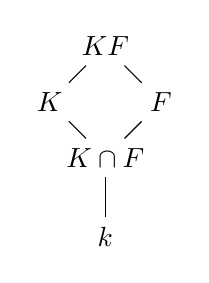
\begin{tikzpicture}
\node (top) at (0,0) {$KF$};	
\node  [below left of=top] (l) {$K$};
\node [below right of=top] (r)  {$F$};
\node  [below right of=l] (c) {$K\cap F$};
\node [below of=c] (c')  {$k$};

\draw (top) -- (l);
\draw (top) -- (r);
\draw (l) -- (c);
\draw (r) -- (c);
\draw (c) -- (c');
\end{tikzpicture}
\]
is a lattice of Galois field extensions.
\end{corollary}

\begin{theorem}
If $K$ is a field with characteristic $0$, $f(x) \in K[x]$ is irreducible, and $L \supset K$ is the splitting field for $f$, then  $f$ is solvable in radicals over $K$ if and only if $\gal(L/K)$ is solvable. 
\end{theorem}
\begin{proof} $ $

($\Longleftarrow$) 

This was proven in \cref{19}.

\medskip

($\Longrightarrow$) 

For any root $\alpha$ of $f$, we can find an extension $K_{\alpha} \supset K$ such that  $\alpha \in L_{\alpha} \subset L$ and there exists a tower of radical extensions $$ K = K_0 \subset K_1 \subset \cdots \subset K_s = K_{\alpha} \subset L$$ with $K_{i+1} = K_i(\alpha_{i+1})$ and $\alpha_{i+1}^{n_{i+1}} \in L_i$. 
\begin{claim}
Without loss of generality, we may assume that $K_{\alpha}$ satisfies the following properties.
\begin{itemize}
\item $\alpha \in K_{\alpha}$.
\item $K_{\alpha} \supset K$ is Galois.
\item Each step of $K_{\alpha}$ (viewed as our tower of radical extensions) is Galois and cyclic. 
\end{itemize}
\end{claim}
\begin{proof}
Since $K_{\alpha}\supset K$ is a finite extension, we can find a $K$-basis $e_1, \ldots, e_n$ of $K_{\alpha}$. Let $f_i \in K[x]$ denote the minimal polynomial of $e_i$. Let $S_i$ denote the splitting field of $f_i$. Then $S_i \supset K$ is a Galois extension and contains $e_i$. Note that the composite of the $S_i$ contains each $e_i$ . Let $L_{\alpha} = S_1S_2 \cdots S_n$. Then $K \subset K_{\alpha} \subset L_{\alpha}$. (We call $L_{\alpha}$ the \textit{Galois closure of $K_{\alpha}$}.) Consider the tower $K = K_0 \subset K_1 \subset \cdots \subset K_s = K_{\alpha}$ where $K_{i+1} \supset K_i$ is a radical extension of degree $n_i$. If $\sigma \in \gal(L_{\alpha}/K)$, then $K = \sigma{K} \subset \sigma{K_1} \subset \cdots \subset \sigma{K_{\alpha}}$ is still a tower of radical extensions. 

\medskip

By taking the composites $K_1\sigma K_1 \subset \cdots \subset K_1\sigma K_s$ and $K_2K_1\sigma{K_1} \cdots$, we get  a composite of all $\left\{\sigma{K}{\alpha}\right\}_{\sigma \in \gal(L_{\alpha}/K)}$, which will be a tower of radical extensions. But $K \subset \prod_{\sigma} \sigma{K_{\alpha}} \subset L_{\alpha}$, and $L_{\alpha}$ is generated by all $\sigma{K_{\alpha}}$. Hence $L_{\alpha} = \prod_{\sigma} \sigma{K_{\alpha}} =L$.

\medskip


We still must prove that each step in our radical tower is Galois and cyclic. Let $n=n_1n_2 \cdots n_k$.  Let $F = K[\mu_n]$. If the tower $K = K_0 \subset K_1 \subset \cdots \subset K_t = L_{\alpha}$ has $K_i = K_{i-1}[\sqrt[n_i]{a_i}]$, then we can pass to composites $$  K \subset K_0F \subset K_1F \subset \cdots \subset K_tF = L_{\alpha}F  .$$ We see that $LF \supset K$ is radical and Galois as the splitting field for $x^n-1$ and that $K_iF \supset K_{i+1}F$ is radical of degree $n_i$ and contains $\mu_{n_i}$. Thus, $K_iF \supset K_{i+1}F$ is Galois and cyclic of degree dividing $n_i$ by \cref{l16}(a). 

\medskip

 We have constructed an extension $LF \supset K$ such that
\begin{itemize}
\item $\alpha \in LF$,
\item $LF \supset L$ is Galois, and
\item $LF$ is a tower of radical, cyclic, Galois extensions.
\end{itemize}
It follows that $\gal(LF/K)$ is solvable. But $LF \supset L \supset K$ where $L \supset K$ is Galois. Hence $\sigma(L) \subset L$ for any $\sigma \in \gal(LF/K)$, so that $\gal(L/K) < \gal(LF/K)$. This proves that $\gal(L/K)$ is solvable.
\end{proof}
\end{proof}

\subsection{Lecture 21}

\begin{definition}
Let $K$ be a field and $f(x) \in K[x]$. We say that $f$ is \textit{solvable in quadratic radicals} if the splitting field $L$ for $f$ is a tower $$K = K_0 \subset K_1 \subset \cdots \subset K_s =L   $$ such that $K_i =K_{i-1}[\sqrt{a_i}]$ for some $a_i \in K_{i-1}$.
\end{definition}

\begin{theorem}\label{solv}
Let $K$ be a field with $\Char{K} \ne 2$ and $f(x) \in K[x]$ be irreducible. Then $f$ is solvable in quadratic radicals if and only if $[L:K] =2^n$ for some $n$ where $L$ denotes the splitting field for $f$.
\end{theorem}
\begin{proof} $ $

($\Longrightarrow$) 

We have that $L \supset K$ is a tower of quadratic extensions. Hence  $[L:K] = 2^n$ for some $n$. 

\medskip


($\Longleftarrow$)  

We have that $[L:K] = 2^n$ for some $n\geq 0$ and $\deg{f} = [K(\alpha): K] \mid [L: K]$ where $\alpha$ is a root of $f(x)$. Thus, $[K(\alpha): K]$ equals a power of $2$, so that $f$ is separable. This shows that $L \supset K$ is Galois and thus that $G\coloneqq  \gal(L/K)$ has order $2^n$. It follows that there is some normal series $$ G =G^0 \unrhd G^1  \unrhd \cdots \unrhd G^s = \{e\}  $$ such that $\faktor{G^{i}}{G^{i+1}} \cong \Z/2$. This induces a tower of field  extensions $$ K= L^{G^0} \subset L^{G_1} \subset \cdots \subset L^{G_s} = L   $$ such that $[L^{G^{i+1}}: L^{G_i}] =2$.
\end{proof}

\smallskip

\begin{note}[The construction problem]
Given a unit measure and segments of lengths $a_1, \ldots, a_k$, we want to construct a segment of length $\alpha$ using ruler and compass. Elementary geometry shows that such a construction is possible if and only if $\alpha$ can be expressed in quadratic radicals over $\Q(a_1, \ldots, a_k)$. 
If $\alpha$ is transcendental over $\Q(a_1, \ldots, a_k)$, then our construction is impossible. 
\begin{exmp}
We see that $\pi$ cannot be constructed over $\Q$, i.e., we cannot square the circle. 
\end{exmp} 
Moreover, if $\alpha$ is algebraic over $\Q(a_1, \ldots, a_k)$, then $\alpha$ can be constructed by \cref{solv} if and only if the minimal polynomial of $\alpha$ has degree power of $2$.
\begin{exmp} $ $
\begin{enumerate}[label=(\alph*)]
\item \underline{Doubling the cube.} Given a segment of length one, construct a segment of length $\sqrt[3]{2}$. Since the minimal polynomial of $\sqrt[3]{2}$ is $x^3-2$, such a construction is impossible.
\item \underline{Trisecting an angle $\varphi$.} Given a segment of length $\cos{\varphi}$, construct a segment of length $\cos\left(\frac{\varphi}{3}\right)$. The minimal polynomial of $\cos\left(\frac{\varphi}{3}\right)$ over $\Q(\cos{\varphi})$ is $4x^3 - 3x - \cos{\varphi}$. In general, this is irreducible, in which case our construction is impossible. 
\item \underline{Constructing regular $n$-gons.} Given a segment of length $i$, construct a segment of length $\cos\left(\frac{2\pi}{n}\right)$. This is possible if and only if $e^{\frac{2\pi i}{n}}$ is expressible in quadratic radicals over $\Q$. In turn, this happens if and only if $$\underbrace{[\Gamma_n : \Q]}_{\varphi(n)} = 2^s.$$ For example, if $p$ is prime, then we can construct a regular $p$-gon if and only if $1+2^k$ for some $k$. Currently, the largest known such $p$ is $\num{65537}$.
\end{enumerate}
\end{exmp}
\end{note}

\section{Further applications of Galois theory}

\subsection{Lecture 22}

To begin, note that the following statements are true.
\begin{itemize}
\item If $f(x) \in \R[x]$ has odd degree, then it has a real root.
\item Every $\alpha \in \C$ has a square root in $\C$.
\end{itemize}
Now, suppose that $K \supsetneq \R$ is a finite field extension. If $[K : \R]$ is odd and $\alpha \in K \setminus \R$, then $K \supset \R(\alpha) \supset \R$, in which case $\deg{f} \mid [K : \R]$ where $f$ denotes the minimal polynomial of $\alpha$ over $\R$.  In this case, $f$ has odd degree and thus has a root in $\R$, so that $\R(\alpha) = \R$, a contradiction. This proves that $[K : \R]$ is odd.

We want to prove the \textit{fundamental theorem of algebra}: that any $f(x) \in \C[x]$ has a root in $\C$. Note that if $c$ is a complex root of $f(x)\overline{f(x)} \in \R[x]$, then either $c$ or $\bar{c}$ is a root of $f(x)$.  Thus, it suffices to show that any polynomial over $\R$ has a root in $\C$.

To this end, let $g(x) \in \R[x]$ be non-constant and irreducible. Let $L$ denote the splitting field for $g$. Then $[L :K] = \left\lvert{\gal(L/\R)}\right\rvert$ is even, so that there is some nontrivial $2$-Sylow subgroup $H \leq \gal(L/\R)$. This means that the intermediate extension $L \supset L^H \supset \R$ has odd degree. But then $L^H = \R$. This means that $L \supset L^H$ is Galois, so that $$\left[L: \R\right] = \left[L: L^H\right] = \left\lvert{\gal(L/L^H)}\right\rvert = \left\lvert{H}\right\rvert = 2^n$$ for some $n$. By \cref{solv}, it follows that $g(x)$ is solvable in quadratic radicals. Therefore, $L = \C$ since $[\C : \R] = 2$. 


\begin{theorem}[Primitive element theorem]
Suppose that $L \supset K$ is a finite field extension. This has a \textit{primitive element}, i.e.,  $L= K(\theta)$ for some $\theta \in L_j$, if and only if there are at most finitely many intermediate fields $K \subset F \subset L$.
\end{theorem}
\begin{proof}
If $K$ is finite, then $L$ is a finite group with cyclic multiplicative group $\langle \theta \rangle$. In this case, we have shown  that $L = K(\theta)$.

\medskip


($\Longleftarrow$) 

For any $\alpha, \beta \in L$, consider the collection of intermediate fields $$K \subset K(\alpha + c\beta) \subset L$$ where $c\in K$. Thus,  $ \exists c, c' \in K$ such that $E\coloneqq  K(\alpha + c \beta) = K(\alpha + c' \beta)$. Hence $(c - c')\beta \in E$, and $c- c' \in K \setminus \{0\}$. Then $ \beta \in E$, so that $\alpha \in E$. This shows that $E \supset K(\alpha, \beta)$. It's clear that $E \subset K(\alpha, \beta)$. Hence $E = K(\alpha, \beta)$. But $L \supset K$ is a finite extension, which implies that $L = K(\alpha_1, \ldots, \alpha_n)$ for some $\alpha_1, \ldots, \alpha_n$. By indiction on $n$, we can find elements $c_2, \ldots, c_n \in K$ such that $$ K(\alpha_1, \ldots, \alpha_n) = K(\alpha_1 + c_2\alpha_2 + c_3\alpha_3 + \cdots + c_n \alpha_n ) . $$

\medskip


($\Longrightarrow$) 

We have that $L= K(\theta)$. Let $f(x) \in K[x]$ denote the minimal polynomial of $\theta$ over $K$. Let $K \subset F \subset L$ be an intermediate field extension. Let $g_F(x) \in F[x]$ denote the minimal polynomial over $F$. This proves that $g_F(x) \mid f(x)$ in $F[x]$. We get a map $$\left(\text{intermediate field extensions } K \subset F \subset L \right) \to \left(\text{divisors of } f(x)\right)$$ given by $F \mapsto g_F(x)$. Since there are at most finitely many divisors of $f(x)$, it suffices to check that this map is injective. 

\medskip

 Suppose that $K \subset F \subset L$. Let $F_0 \subset F$ be the subfield obtained from $K$ by adjoining the coefficients of $g_F(x)$. It is enough to show that $F_0 = F$. Note that $g_F(x)$ is irreducible in $F[x]$, so that $g_F(x)$ is irreducible in $F_0[x]$ Therefore, $g_F(x) \in F_0[x]$, which means that $g_F(x)$ is the minimal polynomial of $\theta$ over $F_0$. Then $[L: F_0] = \deg{g_F} = [L: F]$, so that $F_0 = F$. 
\end{proof}

\begin{corollary}
If $L \supset K$ is a (finite) separable extension, then $L$ has a primitive element. 
\end{corollary}
\begin{proof}
It suffices to show that if $\alpha, \beta \in L$ are separable over $K$, then $K(\alpha, \beta) = K(\theta)$ for some $\theta$. If $K$ is finite, then we're done. Suppose that $K$ is infinite. Let $\varphi_1, \ldots, \varphi_n$ denote the distinct embeddings of $K(\alpha, \beta)$ in $\overline{K}$ over $K$. Consider $$ f(x) = \prod_{i \ne j} (\varphi_i(\alpha) + x \varphi_i(\beta) - \varphi_j(\alpha) - x \varphi_j(\beta))   .$$ Since this is not the zero polynomial, there is some $c\in K$ such that $f(c) \ne 0$. It follows that the $\varphi_i(\alpha + c \beta)$ are pairwise distinct in $\overline{K}$. Then $[K(\alpha + c \beta) : K] \geq n$. But $[K(\alpha, \beta) : K] = n$, so that $K(\alpha, \beta) = K(\alpha + c \beta)$. 
\end{proof}

\smallskip

 Let $K$ be a field and $f(x) \in K[x]$ be a monic separable polynomial. Let $L$ denote the splitting field of $f$, so that $L \supset K$ is Galois. Let $G_f \coloneqq  \gal(L/K) \subset S_n$ where $n = \deg{f}$. Let $\Char{K} \ne 2$.
 
\begin{theorem}
 $L^{G_f \cap A_n} = K(\Delta(f))$ where $\Delta(f) = \prod_{i < j}(\lambda_i - \lambda_j)$ and $\lambda_1, \ldots, \lambda_n$ denote the distinct roots of $f$.
\end{theorem}
Before proving this, note that $\Delta(f)$ is a square root of $\disc(f) \in K$. 
\begin{proof}
Consider $x_1, \ldots, x_n$ purely transcendental elements over $K$. Let $K(x_1, \ldots, x_n) \supset K$ be the corresponding extension. There is a group homomorphism $\Phi : S_n \to \gal(K(x_1, \ldots, x_n)/K)$ given by $\sigma \mapsto \Phi_{\sigma}$ where $$\Phi_{\sigma}(f)(x_1, \ldots, x_n) = f(x_{\sigma^{-1}(1)}, \ldots, x_{\sigma^{-1}(n)}).$$ This is injective, and $K(x_1, \ldots, x_n)^{S_n} = K(\sigma_1, \ldots, \sigma_n)$ where $\sigma_1, \ldots, \sigma_n \in K[x_1, \ldots, x_n]$ are the alternating symmetric polynomials. Further, $\gal(K(x_1, \ldots, x_n)/K(\sigma_1, \ldots, \sigma_n)) = S_n$. Let $\Delta_n = \prod_{i <j}(x_i - x_j) \in K(x_1, \ldots, x_n)$. Then $\Phi_{\sigma}(\Delta_n) = \sgn(\sigma)\Delta_n$, and $\Delta_n \notin K(\sigma_1, \ldots, \sigma_n)$. 

\medskip

 Define $\ev : K(x_1, \ldots, x_n) \to L$ by $x_i \mapsto \lambda_i$. Then $\ev \circ \Phi_{\sigma} = \sigma^{-1} \circ \ev$. Thus, $$\ev(\Delta(f)) = \ev(\Phi_{\sigma}(\Delta_n)) = \sigma^{-1}(\Delta(f)).$$ This shows that the subgroup in $G_f$ fixing $\Delta(f)$ is precisely $G_f \cap A_n$. 
\end{proof}

\begin{corollary}
If $\Char{K} \ne 2$ and $f(x)$ is monic and separable over $K$, then $G_f \subset A_n$ if and only if $\disc(f) \in K^2$. 
\end{corollary}

\subsection{Lecture 23}

\begin{theorem}
Suppose that $K$ is a field and $f(x) \in K[x]$ is separable. Then $f$ is irreducible if and only if the Galois group $G_f$ acts transitively on the set of roots of $f$.  
\end{theorem}
\begin{proof} $ $

 ($\Longrightarrow$) 
 
 For any two roots $\lambda_i, \lambda_j$ of $f$, we have that $K(\lambda_I) \cong K(\lambda_j)$ as fields over $K$ because both $\ev_{\lambda_i} : K[x] \to K(\lambda_i)$ and $\ev_{\lambda_j} : K[x] \to K(\lambda_j)$ induces isomorphisms with $\faktor{K[x]}{(f)}$. By \cref{mlGT}, we can extend this isomorphisms to an automorphism $\sigma : L \to L$ of the splitting field $L$ for $f$. Thus, $\sigma \in \gal(L/K)$ with $\sigma(\lambda_i) = \lambda_j$. 

\medskip


($\Longleftarrow$) 

Let $\left\{\lambda_1, \ldots, \lambda_n\right\}$ denote the set of roots of $f$. Let $f(x) = g(x)h(x)$ where $\deg{g} \geq 1$ and $g$ is irreducible. We must show that $h$ is constant. Let $\lambda$ be any root of $g$. Then there exists $\sigma_i \in G_f$ such that $\sigma_i(\lambda) = \lambda_i$ for each $i=1, \ldots, n$. Note that $$g(\lambda_i) = g(\sigma_i(\lambda))= \sigma_i(g(\lambda)) =0,$$ so that each $\lambda_i$ is a root of $g$. Hence $f \mid g$, which implies that $h$ is constant. 
\end{proof}

\begin{theorem}
Suppose that $p$ is prime and that $f(x) \in \Q[x]$ is monic and irreducible with $\deg{f} =p$. Suppose that $f$ has exactly two non-real roots in $\C$. Then $G_f = S_p$.
\end{theorem}
\begin{proof}
Let $L$ be the splitting field for $f(x)$. Write $f(x) = \prod_{i=1}^p(x- x_i)$ with each $\lambda_i \in \C$. THen $\Q(\lambda_1, \ldots, \lambda_p) \subset \C$. We see that $$ \Q \subset \Q(\lambda_i)  \subset \Q(\lambda_1, \ldots, \lambda_p) \subset \C,$$ so that $[\Q(\lambda_i) : \Q] \mid [L : \Q]$.  Since $p \mid [L: \Q] = \left\lvert{G_f}\right\rvert \subset S_p$, it follows from Sylow that $G_p$ contains an element of order $p$, i.e., that $G_f$ contains a $p$-cycle. Also, the element in $G_f$ that switches the roots is the complex conjugate pair of a transposition.
\end{proof}

\begin{theorem}[Brouwer]
For any prime $p \geq 5$, there are infinitely many polynomials in $\Q[x]$ of degree $p$ with Galois group $S_p$.
\end{theorem}
\begin{proof}
Let $k$ be an odd integer and let $0\leq m, n_1 \leq n_2 < \cdots < n_{k-2}$ be even integers. Consider $$g(x) = (x^2 +m)(x-n_1)(x-n_2) \cdots (x-n_{k-2}).$$ This polynomial has $\frac{k-3}{2}$ local maxima. Also, for each odd $h\in \Z$, $\left\lvert{g(h)}\right\rvert >2$. Hence if $c$ denotes a local maximum of $g$, then $g(c) >2$. This shows that if $f(x) = g(x) -2$, then there are 
\begin{itemize}
\item $\frac{k-3}{2}$ positive local maxima in $[n_1, n_{k-2}]$ and
\item $\frac{k-3}{2}$ negative local maxima in $[n_1, n_{k-2}]$.
\end{itemize}
It follows that $f(x)$ has $k$-3 real roots in $[n_1, n_{k-2}]$ with $f(n_{k-2}) = {-2}$ and $\lim_{x\to \infty} f(x) >0$. Therefore, we have another real roots $> n_{k-2}$. Hence $f(x)$ has at least $k-2$ real roots. Let $\lambda, \ldots, \lambda_n \in \C$ denote the distinct roots of $f$. Then $$\prod_{i=1}^k(x-\lambda_i) = f(x) = (x^2 +m)(x-n_1)(x-n_2) \cdots (x-n_{k-2}) -2$$, and ${-}\sum_{i=1}^k \lambda_i = {- \sum_{i=1}^{k-2} n_i}$. From this, we compute
\begin{align*}
\sum_{i <j} \lambda_i \lambda_j & = m + \sum_{a < b} n_an_b 
\\ \sum_{i=1}^k \lambda_i^2 & = \left(\sum_{i=1}^k \lambda_i \right)^2 = \sum \sum_{i<j} \lambda _i \lambda_j
\\ & = \left( \sum_{i=1}^{k-2} n_i \right)^2 -2m - 2 \left( \sum_{a<b} n_an_b \right)
\\ & = \sum_{i=1}^{k-2} n_i^2 - 2m.
\end{align*}
Choose $m \gg \sum n_i^2$ so that $\sum_{i=1}^k \lambda_i^2  < 0$. This implies that there exists a non-real root. Hence we must have exactly two real roots. Further,  we can write $f(x) = x^k + a_1x^{k-1} + \cdots +a_{k-1} x +a_k$ with each $a_i \in 2\Z$. Since $a_k = f(0) = g(0) -2$, we see that $2 \mid a_{k-1}$ but $4 \nmid a_{k-1}$. By Eisenstein's criterion, $f$ must be irreducible. We thus get infinitely many $f$'s such that $G_f = S_p$. 
\end{proof}

\section{Chain complexes and chain maps}

The originators of homological algebra include Betti, Poincar\'e, and Riemann. The main goal of this subject is to extract invariants from topological spaces. Decompose $X$ into contractible pieces (such as cells or simplices) to reduce $X$ to combinatorial data. Specifically, reduce $X$ to a collection of pieces of various dimensions where the boundary of a piece of dimension $n$ is glued to a sub-collection of pieces of dimension $n-1$. 

Emmy Noether introduced groups of chains $C_i(X)$, a free abelian group generated by the collection of $i$-dimensional pieces, equipped with boundary relations $\partial_i : C_i(X) \to C_{i-1}(X)$. From this, we obtain abelian groups $H_i(X)\equiv \faktor{\ker{\partial_i}}{\im{\partial_{i+1}}}$, which are algebraic invariants of $X$. 

Hilbert wanted to extract numerical invariants from a module. Specifically, if $k$ is a field and $K\coloneqq  k[x_1, \ldots, x_n]$, then he wanted to understand the complexity of a module over $K$ (or, more generally, any graded module  over $k$).

\bigskip

A typical graded module over $R$ will be a module of the form $M R/I$ where $I \unlhd R$ is a homogeneous ideal. By the Hilbert basis theorem, $I \unlhd R$ is generated by finitely many homogenous polynomials $f_1, f_2, \ldots, f_{r_0}$. Thus, we have surjective map $\psi: R^{\oplus r_o} \to I $ given by $(a_1, \ldots, a_{r_0}) \mapsto \sum a_if_i$. But, there generators are not, in general, independent. Therefore, we consider the module of relations $Z_0(I) \equiv \ker{\psi}$ among the $f_i$. Note that $Z_0(I)$ is finitely generated. We can choose generators and get a map $\psi': R^{\oplus r_1} \twoheadrightarrow Z_0(I)$. Then $$R^{\oplus r_1} \to R^{\oplus r_0} \to I \to 0$$ is an exact sequence of graded $R$-modules. If $Z_1(I) \equiv \ker{\psi'}$ is not zero, then choose generators again to get a map $\psi'': R^{\oplus r_2} \twoheadrightarrow Z_1(I)$. Continuing in this way, we get an exact sequence $$\cdots \to R^{\oplus r_2} \to R^{\oplus r_1} \to R^{\oplus r_0} \to I \to 0.$$ The \textit{length} of this sequence is defined to be $\max\{i \mid r_i \ne 0\}$. This is an invariant of $I$ and of $R/I$.


\begin{theorem}[Hilbert's syzygy theorem]
Hilbert's syzygy theorem states that $Z_{n-1}(I)$ is free, i.e., that there is an exact sequence of graded $R$-modules $$0 \to R^{\oplus r_n} \to R^{\oplus r_{n-1}} \to \cdots \to R^{\oplus r_0} \to I \to 0.$$
\end{theorem}

\subsection{Lecture 24}

\begin{definition} $ $
\begin{enumerate}
\item  A \textit{chain complex} (in $\mathbf{Ab}$) is a pair $\left(M_{\bullet}, \partial_{\bullet}\right)$ where $M_{\bullet} = \{M_i\}_{i\in \Z}$ is a set of abelian groups and $\partial_{\bullet} =\{\partial_i\}_{i\in \Z}$ is a set of morphisms in $\mathbf{Ab}$ such that the \textit{$i$-th differential} $\partial_i : M_i \to M_{i-1}$ satisfies $\partial_{i-1} \circ \partial_i = 0$. 

We call $Z_n \equiv \ker{\partial_{n}}$ \textit{the group of degree $n$ cycles} and $B_n \equiv \im{\partial_{n+1}}$ \textit{the group of degree $n$ boundaries}. Finally, we call $H_n \equiv Z_n/B_n$ the \textit{degree $n$ homology group}.
\item A \textit{((co)chain) complex} (in $\mathbf{Ab}$) is a pair $\left(M^{\bullet}, d^{\bullet}\right)$ where $M^{\bullet} = \{M^i\}_{i\in \Z}$ is a set of abelian groups and $d^{\bullet} =\{d^i\}_{i\in \Z}$ is a set of morphisms in $\mathbf{Ab}$ such that the \textit{$i$-th differential} $d^i : M^i \to M^{i+1}$ satisfies $d^{i+1} \circ d^i = 0$. 

We call $Z^n \equiv \ker{d^n}$ \textit{the group of degree $n$ cocycles} and $B^n \equiv \im{d^{n-1}}$ \textit{the group of degree $n$ coboundaries}. 

Finally, we call $H^n \equiv Z^n/B^n$ the \textit{degree $n$ cohomology group}.
\end{enumerate}
\end{definition}

\begin{definition} Let $\left(A^{\bullet}, d_A^i\right)$ and $\left(B^{\bullet}, d_B^i\right)$ be complexes.
 A \textit{chain map} $f^{\bullet} : \left(A^{\bullet}, d_A^{\bullet}\right) \to \left(B^{\bullet}, d_B^{\bullet}\right)$ consists of group homomorphisms $f^i : A^i \to B^i$ for each $i\in \Z$ such that $d_B^i \circ f^i = f^{i+1} \circ d^i_A$. 
\end{definition}

\begin{note} $ $
\begin{enumerate}
\item Any chain map $f^{\bullet}: \left(A^{\bullet}, d_A^{\bullet}\right) \to \left(B^{\bullet}, d_B^{\bullet}\right)$ restricts term-wise to maps $f^i :Z^i(A^{\bullet}) \to Z^i(B^{\bullet})$ and maps $f^i : B^i(A^{\bullet}) \to B^i(B^{\bullet})$. Thus, it induces a map $f^{\ast} : H^i(A^{\bullet}) \to H^i(B^{\bullet})$.
\item We have a natural isomorphism $\mathbf{Ch}(\mathbf{Ab}) \to \mathbf{CoCh}(\mathbf{Ab})$ given by $N_i \mapsto M^{-i}$ and $\partial_i \mapsto d^{-i}$.
\end{enumerate}
\end{note}

\begin{definition}
We say that $\left(A^{\bullet}, d^{\bullet}\right)$ is \textit{bounded above} if there is some $N$ such that $A^n =0$ for any $n\geq N$. We define \textit{bounded below} similarly. We say that $\left(A^{\bullet}, d^{\bullet}\right)$ is \textit{bounded} if it is both bounded above and bounded below. 
\end{definition}

As a result, we have the subcategories $\mathbf{CoCh}^{{-}}(\mathbf{Ab})$, $\mathbf{CoCh}^{+}(\mathbf{Ab})$, and $\mathbf{CoCh}^{b}(\mathbf{Ab})$, respectively. 

\medskip


If $C^{\bullet} = \bigoplus_{i\in \Z} C^i$ is a graded abelian group, then it induces a natural complex $(\underline{C}^{\bullet}, 0)$ where $\underline{C}^i \equiv C^i$. In particular, any abelian group may be viewed as a complex. 

Conversely, given a complex $(M^{\bullet}, d^{\bullet})$, we can form the graded abelian group $M^{\bullet} \equiv  \bigoplus_{i\in \Z} M^i$ and package the differential $d^i$ into a single group map $D: M^{\bullet} \to M^{\bullet}$ such that $D\restriction_{M^i} = d^i$ and $D^2 =0$. We can write $D$ as the block diagonal matrix
$$  \begin{bmatrix} 0 & & &  & \\  d^i &0   &  &  & \\  &  d^{i+1} & 0  &   & \\ &   & d^{i+2}  & 0   &   \\  &  & &  \ddots &   \ddots \end{bmatrix} .$$
As a result, we obtain the \textit{cochain functor} given by $\left(A^{\bullet}, d^{\bullet}\right) \to \bigoplus_{i\in \Z} A^i$ and $f^{\bullet} \mapsto (f^i)_{i\in \Z}$.



\begin{definition}
We say that $\left(A^{\bullet}, d^{\bullet}\right)$ is \textit{acyclic} or \textit{exact} if $H^{\bullet}\left(A^{\bullet}, d^{\bullet}\right)=0$.
\end{definition}

\medskip

\begin{theorem}
Let $K^{\bullet}$ be an exact complex of $R$-modules and $I^{\bullet}$ a bounded below complex of injective $R$-modules. Any chain map $f: K^{\bullet} \to I^{\bullet}$ is homotopic to zero.
\end{theorem}
\begin{proof}
There is some $r\in \Z$ such that $I^k =0$ for any $k<r$. Then $f^k =0$ for any $k<r$. Define $h^k: K^k \to I^{k-1}$ by $h^k =0$ for each $k\leq r$. Then $f^{k} = 0 = d_I{h^{k}} + h^{k+1}{d_K}$ for any $k <r$. Let $s> r$ and assume, for induction, that, for each $k<s$, we have constructed $h^k : K^k \to I^{k-1}$ such that $f^{k-1} = d_I{h^{k-1}} + h^{k}{d_K}$. We must construct $h^s : K^s \to I^{s-1}$ such that $f^{s-1} = d_I{h^{s-1}} + h^{s}{d_K}$.
\\ \\ Let $g^{s-1} = f^{s-1} - d_I{h^{s-1}}$. Note that 
\begin{align*}
g^{s-1}{d_K} & = \left(f^{s-1} - d_I{h^{s-1}}\right){d_K}
\\ & = f^{s-1}{d_K} -  d_I{h^{s-1}}{d_K}
\\ & = d_I{f^{s-2}} - d_I\left(f^{s-2} - d_Ih^{s-2}\right)
\\ & = 0.
\end{align*}
Therefore, $g^{s-1}$ descends to a map ${g}^{s-1} : \faktor{K^{s-1}}{\im{d_K}} \to I^{s-1}$. Since $K^{\bullet}$ is exact, we have $${g}^{s-1} : \faktor{K^{s-1}}{\ker{d_K}} \to I^{s-1}.$$ Moreover, since $I^{s-1}$ is injective, we can find some map $h^s : K^s \to I^{s-1}$ such that
\[
\begin{tikzcd}
I^{s-1}                                                              &                          &                                 \\
\faktor{K^{s-1}}{\ker{d_K}} \arrow[u, "g^{s-1}"] \arrow[r, "\cong"'] & \im{d_K} \arrow[r, hook] & K^s \arrow[llu, "h^s"', dashed]
\end{tikzcd}
\] commutes. Hence $h^s{d_K} = g^{s-1}$. It follows that
\begin{align*}
  d_I{h^{s-1}} + h^{s}{d_K} & = d_I{h^{s-1}} + g^{s-1}
\\ & = d_I{h^{s-1}} + f^{s-1} - d_I{h^{s-1}}
\\ & = f^{s-1},
\end{align*}
as desired
\end{proof}

\medskip

\begin{definition}
If $A$ is an abelian group, then a \textit{left resolution of $A$} is an exact complex $(C^{\bullet}, d^{\bullet}) \in \ob{\mathbf{CoCh}^{\leq 0}(\mathbf{Ab})}$  of the form $$\cdots \to C^{i-1} \to C^i \to \cdots \to  C^0 \to A \to 0 .$$
\end{definition}

\begin{exmp}
If $I \unlhd k[x_1, \ldots, x_n]$ is a homogenous ideal, then Hilbert's syzygy theorem says that $I$ has a left resolution of length $n+1$ with $n+1$ terms free finitely generated $R$-modules.
\end{exmp}

\smallskip

Let $a\in \Z$. Define the \textit{shift functor} $${-}[a] : \mathbf{CoCh}(\mathbf{Ab}) \to \mathbf{CoCh}(\mathbf{Ab})$$ as follows. Let $\left(M^{\bullet}, d^{\bullet}_{M}\right)$ be a complex.  Form the pair $\left(M^{\bullet}[a], d^{\bullet}_{M[a]}\right)$ where $\left(M^{\bullet}[a]\right)^n \equiv M^{a+n}$ and $\left(d_{M[a]}\right)^n \equiv ({-1})^a d^{a+n}_M$. If $f^{\bullet}$ is a chain map, then let $\left(f^{\bullet}[a]\right)^n = f^{a+n}$.


\begin{prop}
The shift functor  is an equivalence that preserves $\mathbf{CoCh}^{{-}}(\mathbf{Ab})$, $\mathbf{CoCh}^{+}(\mathbf{Ab})$, and $\mathbf{CoCh}^{b}(\mathbf{Ab})$.
\end{prop}

\begin{definition}
Let $f: M \to N$ be a chain map. Form  $\cone(f)$ the \textit{cone of $f$} as a new complex where $\cone(f)^{\bullet} \equiv N \oplus M[1]$ and $d_{\cone(f)}^{\bullet} \equiv \begin{bmatrix}  d_N & f \\ 0 & d_{M[1]}    \end{bmatrix}.$
\end{definition}


We see that $$\cone(f)^n = N^n \oplus M^{n+1}$$ and $d^n_{\cone(f)} : N^n \oplus M^{n+1} \to N^{n+1} \oplus M^{n+2}$ with $$d^n_{\cone(f)}  = \begin{bmatrix}  d_N^n & f^{n+1} \\ 0 & {-d_M^{n+1}}  \end{bmatrix}.$$


\begin{exercise}
Show that $d^{i+1}_{\cone(f)} \circ d^i_{\cone(f)} =0$.
\end{exercise}

\begin{definition} $ $
\begin{enumerate}
\item A \textit{double complex} is a triple $\left(A^{\bullet, \bullet}, d^{\bullet}, \delta^{\bullet}\right)$ where $A^{i,j} = \{A^{i,j}\}_{(i,j) \in \Z^2}$ and both $d : A^{\bullet, \bullet} \to A^{\bullet +1, \bullet}$ and $\delta : A^{\bullet, \bullet} \to A^{\bullet, \bullet +1}$ are homomorphisms such that $d{\delta} = \delta{d}$ and $d^2 = \delta^2 =0$.
As a commutative diagram, this has the form
 \[
\begin{tikzcd}
                           & \vdots \arrow[d, "d"]                           & \vdots \arrow[d, "d"]                            & \vdots \arrow[d, "d"]                            &        \\
\cdots \arrow[r, "\delta"] & {A^{p,q}} \arrow[d, "d"] \arrow[r, "\delta"]    & {A^{p,q+1}} \arrow[d, "d"] \arrow[r, "\delta"]   & {A^{p,q+2}} \arrow[r, "\delta"] \arrow[d, "d"]   & \cdots \\
\cdots \arrow[r, "\delta"] & {A^{p+1, q}} \arrow[d, "d"] \arrow[r, "\delta"] & {A^{p+1,q+1}} \arrow[d, "d"] \arrow[r, "\delta"] & {A^{p+1,q+2}} \arrow[r, "\delta"] \arrow[d, "d"] & \cdots \\
\cdots \arrow[r, "\delta"] & {A^{p+2, q}} \arrow[r, "\delta"] \arrow[d, "d"] & {A^{p+2,q+1}} \arrow[r, "\delta"] \arrow[d, "d"] & {A^{p+2,q+2}} \arrow[r, "\delta"] \arrow[d, "d"] & \cdots \\
                           & \vdots                                          & \vdots                                           & \vdots                                           &       
\end{tikzcd}
.\]
\item The \textit{total complex of $\left(A^{\bullet, \bullet}, d^{\bullet}, \delta^{\bullet}\right)$} is the complex $ \tot(A)$ where $\tot(A)^n \equiv \bigoplus_{p+q =n} A^{p,q}$ and $d_{\tot(A)}\restriction_{A^{p,q}} \equiv d + ({-1})^p \delta$. 
\end{enumerate}
\end{definition}

\begin{prop}
Any chain map $f: M \to N$ induces a double complex 
\[
\begin{tikzcd}
{M^{i-1, 0}} \arrow[d, "f"] \arrow[r, "d_M"] & M^{i,0} \arrow[d, "f"] \arrow[r, "d_M"] & M^{i+1,0} \arrow[d, "f"] \arrow[r, "d_M"] & M^{i+2,0} \arrow[d, "f"] \arrow[r, "d_M"] & \cdots \\
{N^{i-1,1}} \arrow[r, "d_N"]                 & N^{i,1} \arrow[r, "d_N"]                & N^{i+1,1} \arrow[r, "d_N"]                & N^{i+2,1} \arrow[r, "d_N"]                & \cdots
\end{tikzcd}
.\]
The total complex of this is precisely $\cone(f)$.
\end{prop}

\smallskip

 Let $N$ and $C$ be complexes. Suppose that $C \overset{\iota}{\longrightarrow} N$ is a chain map where each $\iota^n :N^n \to C^n$ is injective. Let $s^n : C^n \to N^n$ be a group homomorphism such that $s^n \circ \iota^n = \id_{N^n}$. Then $M\coloneqq  \left(C/N, d_{C/N}\right)$ is a complex. Our choice of $s^n$ produces a splitting $C^{\bullet} \cong N^{\bullet} \oplus M^{\bullet}[1]$ in the category of  graded abelian groups. Thus, we have the map $d_C = \begin{bmatrix} d_N & f \\ 0 & d_{M[1]} \end{bmatrix}$ where $f: M \to N$ is a map of graded abelian groups.

\begin{exercise} 
 Show that $f$ is a chain map and $C \cong \cone(f)$.
\end{exercise}

\subsection{Lecture 25}

\begin{definition}
Let $f, g : A^{\bullet} \to B^{\bullet}$ be two chain maps. A \textit{homotopy between $f$ and $g$} is a map of graded abelian groups $h: A^{\bullet} \to B^{\bullet -1}$ such the $$d_Bh + hd_A = f-g. $$ We say that $f$ and $g$ are \textit{homotopy equivalent} (written as $f \sim g$) if there is a homotopy between them.
\end{definition}

\begin{prop} $ $
\begin{enumerate}
\item Homotopy is an equivalence relation. 
\item The class $\mor^{\sim{0}}{\mathbf{CoCh(Ab)}}$ of all chain maps homotopic to $0$ is a two-sided ideal in  $\mor{\mathbf{CoCh(Ab)}}$. 
\item If $ f \simeq g: A^{\bullet} \to B^{\bullet}$, then $H^{\bullet}(f) = H(^{\bullet}g)$.
\item If $f\simeq g$ and $c$ is a cocycle, then $f(c) - g(c) = d_Bh(c)$, which is a coboundary.
\end{enumerate}
\end{prop}

\begin{notation}
Let $\mathcal{C}(\mathbf{Ab})$ denote the category with complexes as objects and homotopy classes of chain maps as morphisms.  
\end{notation}

\begin{note} $ $
\begin{enumerate}
\item We have that $\Hom_{\mathcal{C}(\mathbf{Ab})}(A, B) = \faktor{\Hom_{\mathbf{CoCh(Ab)}}(A, B)}{\Hom_{\mathbf{CoCh(Ab)}}^{\sim 0}}(A, B)$.
\item $H^{\bullet}$ descends to a well-defined functor in the sense that the diagram
\[
\begin{tikzcd}
 \mathbf{CoCh(Ab)} \arrow[d, "H^{\bullet}"'] \arrow[r] &  \mathcal{C}(\mathbf{Ab}) \arrow[ld, "H^{\bullet}"] \\
\mathbf{grAb}                                          &                                  
\end{tikzcd}
. \]
commutes.
\end{enumerate}
\end{note}

\begin{definition}
A \textit{short exact sequence of complex} is a sequence $0 \to A \overset{f}{\longrightarrow} B \overset{g}{\longrightarrow} C \to 0$ of complexes such that each sequence $$0 \to A^n \overset{f^n}{\longrightarrow} B^n \overset{g^n}{\longrightarrow} C^n \to 0$$ is exact in $\mathbf{Ab}$.
\end{definition}


Let $$0 \to A \overset{f}{\longrightarrow} B \overset{g}{\longrightarrow} C \to 0$$ be a short exact sequence of complexes. Consider the commutative diagram
 \[
 \begin{tikzcd}
0 \arrow[r] & A^{n-1} \arrow[r, "f^{n-1}"] \arrow[d, "d^{n-1}_A"'] & B^{n-1} \arrow[r, "g^{n-1}"] \arrow[d, "d_B^{n-1}"] & C^{n-1} \arrow[r] \arrow[d, "d_C^{n-1}"] & 0 \\
0 \arrow[r] & A^n \arrow[r, "f^n"] \arrow[d, "d_A^n"']             & B^n \arrow[r, "g^n"] \arrow[d, "d_B^n"]             & C^n \arrow[r] \arrow[d, "d_C^n"]         & 0 \\
0 \arrow[r] & A^{n+1} \arrow[r, "f^{n+1}"]                         & B^{n+1} \arrow[r, "g^{n+1}"]                        & C^{n+1} \arrow[r]                        & 0
\end{tikzcd}
 .\]
 Define a collection of \textit{edge homomorphisms} $\left\{\delta^n : H^n(C) \to H^{n+1}(A)\right\}_{n\in \Z}$ as follows. Let $c\in C^n$ with $d_C^n(c) =0$. By exactness, there is some $b\in B^n$ such that $g^n(b) =c$. But then $$d_B^n(b) \in \ker{g^{n+1}} = \im{f^{n+1}}.$$ Since $f^{n+1}$ is injective, this means that there is a unique $a \in A^{n+1}$ such that $f^n(a) = d_B^n(b)$. Let $\delta^n([c]) = [a]$.


\begin{exercise}
Check that $\delta^n$ is a homomorphism and that it is independent both of our choice of $c$ and of our choice of $b$. 
\end{exercise}

\begin{lemma}[Snake]\label{snake}
Any short exact sequence $$0 \to A \overset{f}{\longrightarrow} B \overset{g}{\longrightarrow} C \to 0$$  complexes induces a \textit{long exact sequence in cohomology}
\[
\begin{tikzcd}
                                  & \cdots \arrow[r]              & H^{n-1}(C) \arrow[lld, "\delta^{n-1}"'] \\
H^n(A) \arrow[r, "f^{\ast}"']     & H^n(B) \arrow[r, "g^{\ast}"'] & H^n(C) \arrow[lld, "\delta^n"]          \\
H^{n+1}(A) \arrow[r, "f^{\ast}"'] & H^{n+1}(B) \arrow[r]          & \cdots                                 
\end{tikzcd}
.\]
\end{lemma}
\begin{proof} $ $

\smallskip

\underline{Exactness at $H^n(B)$:}
We have that $0_{H^n(C)} = H^n(0) = H^n(g \circ f) = H^n(g) \circ H^n(f)$. Hence $\im{H^n(f)} \subset \ker{H^n(g)}$.

For the reverse inclusion, let $[b] \in \ker{H^n(g)} \subset H^n(B)$. Then $g(b) \in C^n$ must be a coboundary, so that there is some $c\in C^{n-1}$ such that $g(b) = d_C{c}$. Choose a lift $b_1 \in B^{n-1}$ of $c$, meaning that $g(b_1) = c$. Then $b -  d_B{b_1} \in Z^n(B)$, and $[b] = [b - d_B{b_1}]$. But $$g(b - d_B{b_1}) = g(b) - g(d_B{b_1}) = g(b) - d_C{g(b_1)} = g(b) - d_C{c} =0.$$ Hence $b - d_B{b_1} \in \ker{g} \subset B^n$. This implies that there exists a unique $a \in A^n$ such that $b- d_B{b_1} = f(a)$. Also, $$   f(d_A{a}) = d_B(f(a)) = d_B(b-d_B{b_1}) = 0   .$$ Since $f$ is injective, we see that $d_A{a} =0$, i.e., $a \in Z^n(A)$. Thus, $H^n(f)([a]) = [f(a)] = [b-d_B{b_1}] = [b]$. This proves that $[b] \in \im{H^n(f)}$.

\medskip


\underline{Exactness at $H^n(C)$:} Let $[b] \in H^n(B)$. Note that $\delta^n(H^n(g)([b])) = [a]$ where $a\in A^{n+1}$ denotes the unique element such that $f(a) = d_B{b} $. Since $d_B{b} =0$ and $f$ is injective, it follows that $a=0$. Hence $\im{H^n(g)}\subset \ker{\delta^n}$.  

Conversely, let $[c] \in \ker{\delta^n}$. Choose $b\in B^n$ such that $g(b) =c$ and then the unique $a\in A^{n+1}$ such that $f(a) = d_B{b}$. Thus, $\delta^n([c]) =[a] =0$, so that $a\in B^{n+1}(A)$, i.e., $d_A{a_1} =a$ for some $a_1 \in A^n$. Note that $g(b-f(a_1))= g(b) -g(f(a_1)) = c -0 =c$. Further, 
\begin{align*}
d_B(b-f(a_1)) & = d_B(b) - d_B(f(a_1))
\\ & = f(a) - f(d_A{a_1})
\\ & = f(a) - f(a)
\\ & =0.
\end{align*} 
This shows that $b-f(a_1)$ is a cocycle. Thus, $H^n(g)([b-f(a_1)]) = [g(b- f(a_1))] = [c]$, so that $[c] \in \im{H^n(g)}$. 

\medskip


\underline{Exactness at $H^{n+1}(A)$:} Let $[c] \in H^n(C)$ and find $[a] = \delta^n([c])$, where
\[
\begin{tikzcd}
                 & b \arrow[d] \arrow[r, "g"] & c \\
a \arrow[r, "f"] & d_B{b}                     &  
\end{tikzcd}
.\] 
Then $H^{n+1}(f)([a]) = [f(a)] = [d_B{b}] =0$. It follows that $\im{\delta^n} \subset \ker{H^{n+1}(f)}$.

Conversely, let $[a] \in  \ker{H^{n+1}(f)}$, so that $H^{n+1}(f)([a]) = [f(a)]= 0$. This means that $f(a) = d_B{b}$ for some $b \in B^n$. Then $\delta^n([g(b)]) = [a]$. This shows that $\im{\delta^n} \supset \ker{H^{n+1}(f)}$.
\end{proof}

\section{Additive categories}

\begin{definition} $ $
\begin{enumerate}
\item A category $\c$ is \textit{enhanced over $\mathbf{Ab}$} if $\Hom_{\c}(a, b)$ is an abelian group for any $a, b \in \ob{\c}$ and $$\Hom_{\c}(y, z) \times \Hom_{\c}(x,y) \overset{\circ}{\longrightarrow} \Hom_{\c}(x,z)$$ is bilinear for any $x,y,z\in \ob{\c}$.
\item A category $\c$ is called \textit{additive} if it is enhanced over $\mathbf{Ab}$ and has finite products. 
\end{enumerate}
\end{definition}

\begin{exmp} The following are additive categories. 
\begin{enumerate}
\item $\mathbf{Ab}$.
\item $R{-}\mathbf{Mod}$.
\end{enumerate}
\end{exmp}

\begin{note} $ $
\begin{enumerate}
\item Let $\c$ be category with finite products. The product of the empty diagram is the terminal object in $\c$ since it is the initial object in $\mathbf{Set}$.
\item If $\c$ is additive and $\ast$ is the terminal object in $\c$, then $\Hom_{\c}(\ast,\ast)$ consists of a single element, which must equal the group identity element.
\end{enumerate}
\end{note}

\begin{exercise} Verify the following statements.
\begin{enumerate}
\item If $\c$ is a additive, then its terminal object is also initial and thus is a \textit{zero object} in $\c$. 
\item A zero object $0_{\c}$ satisfies $\Hom_{\c}(x, 0_{\c}) =0$ and $\Hom_{\c}(0_{\c}, x) =0$ for any $x\in \ob{\c}$.
\item Any additive category has finite coproducts that are equal to finite products.
\end{enumerate}
\end{exercise}

\subsection{Lecture 26}

\begin{definition}
Let $\c$ be an additive category. Let $f: x \to y$ be a morphism in $\c$. 
\begin{enumerate}
\item A \textit{kernel (object) for $f$} is a pair $(k, q)$ where $k \in \ob{\c}$ and $q : k \to x$ such that for any $z \in \ob{\c}$, the natural sequence $$ \Hom(z,k) \overset{q\circ {-}}{\longrightarrow} \Hom(z,x) \overset{f\circ {-}}{\longrightarrow} \Hom(z,y)   $$ is exact.
\item  A \textit{cokernel (object) for $f$} is a pair $(c, p)$ where $c \in \ob{\c}$ and $p : y \to c$ such that for any $z \in \ob{\c}$, the natural sequence $$ \Hom(c,z) \overset{{-}\circ p}{\longrightarrow} \Hom(y,z) \overset{{-}\circ f}{\longrightarrow} \Hom(x,z)   $$ is exact.
\end{enumerate}
\end{definition}

\begin{definition}
We say that a category $\a$ is \textit{abelian} if
\begin{enumerate}
\item $\a$ is additive and
\item for any morphism $f : x \to y$ in $\a$, there exists a sequence $k \overset{q}{\longrightarrow} x  \overset{a}{\longrightarrow} i \overset{b}{\longrightarrow}y \overset{p}{\longrightarrow} c$ in $\a$ such that
\begin{enumerate}
\item $(k, q)$ is a kernel for $f$,
\item $(c, p)$ is a cokernel for $f$,
\item $(c, a)$ is a cokernel for $q$, and
\item $(i,b)$ is a kernel for $p$.
\end{enumerate}
We call $i$ the \textit{image of $f$}.
\end{enumerate}
\end{definition}

\begin{definition}
If $\a$ is a abelian, then a sequence $x \overset{f}{\longrightarrow} y \overset{g}{\longrightarrow} z$ in $\a$ is \textit{exact} if $\im{f} = \ker{g}$.
\end{definition}

\begin{exmp} $ $
\begin{enumerate}
\item $\mathbf{Ab}$.
\item $R{-}\mathbf{Mod}$.
\item $\mathbf{PreShAb}_X$ where $X$ is a space.
\end{enumerate}
\end{exmp}

\begin{remark}
Our notion of and results for cohomology for complexes of abelian groups hold for complexes of objects in an abelian category.
\end{remark}

\begin{theorem}[Freyd-Mitchell]
Every abelian  category admits a fully faithful embedding into $R{-}\mathbf{Mod}$ for some ring $R$.
\end{theorem}

\begin{remark}
It is not, in general, possible to complete an additive category $\c$ to an abelian one. Still, we can always add enough images to $\c$ to get cones of maps of complexes.
\end{remark}

\smallskip

Let $\c$ be additive. A map $e: x\to x$ in $\c$ is an \textit{idempotent} if $e^2=e$. Let $\c= \mathbf{Vect}_k$. Then an idempotent map $e : x \to x$ is a projection map, i.e., $x = x_1 \oplus x_2$ such that $e = i_1 \circ p_1$.



If $\c$ is additive and $e: x \to x$ is idempotent in $\c$, then we say that $e$ \textit{has an image in $\c$} if there exists a decomposition $x = x_1 \oplus x_2$ such that $$e = \begin{bmatrix} \id_{x_1} & 0 \\ 0 & 0   \end{bmatrix}    $$ with respect to this decomposition. We say that $x_1$ is the \textit{image of $e$}.



Let $e : x \to x$ be an idempotent. Then $\id_{x}{e} : x \to x$ is also an idempotent. Indeed, $$ (\id_x - e)^2 = \id_x^2 - \id_x{e} - e {\id_x} + e^2 = \id_x = e   .$$ If $x = x_1 \oplus x_2$ has $e = \begin{bmatrix}  \id_{x_1} & 0 \\ 0 & 0 \end{bmatrix}$, then $\id_x - e = \begin{bmatrix}  0 & 0 \\ 0 & \id_{x_2} \end{bmatrix}$, so that $\id_x - e$ has $x_2$ as an image.


\begin{definition}
A category $\c$ is \textit{idempotent complete} or \textit{Karoubian} if $\c$ is additive and any idempotent in $\c$ has an image in $\c$.
\end{definition}

\begin{exercise}
Show that for any additive category $\c$, there exists a unique (up to unique isomorphism) category $\c^{\kor}$ together with a functor $F : \c \to \c^{\kor}$ such that 
\begin{enumerate}
\item $\c^{\kor}$ is idempotent complete,
\item $F$ is fully faithful, and
\item every object in $\c^{\kor}$  is an image of an idempotent in $\c$.
\end{enumerate}
\end{exercise}

\begin{definition}
A \textit{graded additive category} is an additive category $\c$ such that for any $x,y \in \ob{\c}$, $\Hom(x,y)$ is a graded abelian group, i.e., $\Hom(x,y) \cong \bigoplus_{n \in \Z} \Hom^n(x,y)$ and $\Hom(x,y) \times \Hom(y,z) \overset{\circ}{\longrightarrow} \Hom(x,z)$ has the form $\Hom^n(x,y) \times \Hom^m(y,z) \overset{\circ}{\longrightarrow} \Hom^{n+m}(x,z)$ where $\circ$ is bilinear. 
\end{definition}

\begin{definition}
A graded additive category $\c$ is a \textit{differential graded category} if for any $x,y \in \ob{\c}$, the graded group $\Hom(x,y)$ is equipped with with a homomorphism $d : \Hom(x,y) \to \Hom(x,y)$ such that
\begin{enumerate}[label=(\alph*)]
\item $d : \Hom^n(x,y) \to \Hom^{n+1}(x,y)$,
\item $d^2 =0$, and
\item $d$ satisfies the \textit{graded Leibniz rule}, i.e., if $f \in \Hom^n(x,y)$ and $g \in \Hom(a,x)$, then $$  d(f\circ g) = df\circ g +({-1})^nf \circ dg  .$$
\end{enumerate}
\end{definition}

\begin{prop} Let $\c$ be a category.
\begin{enumerate}
\item If $\c$ is additive, then for any $x\in \ob{\c}$, $\Hom(x,x)$ is a ring (in fact, a $\Z$-algebra).
\item If $\c$ is a graded additive category, then for any $x\in \ob{\c}$, $\ed(x)$ is a graded ring.
\item If $\c$ is differential graded category, then for any $x\in \ob{\c}$, $\ed(x)$ is a differential graded algebra.
\end{enumerate}
\end{prop}

\begin{definition}
If $\c$ is a differential graded category, then the \textit{homotopy category of $\c$} is the category $\ho(\c)$ (or $\left[\c\right]$) given by 
\begin{align*}
\ob{\ho(\c)} & \equiv \ob{\c}
\\  \Hom_{\ho(\c)}(x,y) & \equiv H^0(\Hom_{\c}(x,y), d)
\\ & =\frac{   \ker(\Hom^0_{\c}(x,y) \overset{d}{\longrightarrow} \Hom_{\c}^1(x,y))  }{  \im(\Hom_{\c}^{-1}(x,y) \overset{d}{\longrightarrow} \Hom_{\c}^0(x,y))      }.
\end{align*}
\end{definition}

\medskip

 Let $\b$ be an additive category. Define the category  $\mathbf{Compl}(\b)$  of complexes in $\b$ by 
\begin{align*}
\ob{\mathbf{Compl}(\b)} & = \left(\text{complexes of objects in } \b\right)
\\ \mor{\mathbf{Compl}(\b)} & = \left(\text{morphisms of complexes}\right).
\end{align*}
This is an additive category. We can also refine this definition by incorporating degree-shifting maps to get a differential graded category of complexes in $\b$. Define the category $\mathbf{Compl}^{\bullet}(\b)$ by 
\begin{align*}
\ob{\mathbf{Compl}^{\bullet}(\b)} & = \left(\text{complexes of objects in } \b\right)
\\ \Hom_{\mathbf{Compl}^{\bullet}(\b)}(M, N) & = \bigoplus_{n \in \Z}\Hom^n(M, N)
\end{align*}
where $$ \Hom^n(M , N) \equiv \prod_{a\in \Z} \Hom_{\b}(M^a, N^{a+n})  .$$  The composition is obtained component-wise from the composition in $\b$. Define $d : \Hom^n(M, N) \to \Hom^{n+1}(M, N)$ by $$ \left(f_a\right)_{a\in \Z} \to \left(d_N \circ f_a + ({-1})^n f_{a+1} \circ d_M\right)_{a\in \Z}  .$$ This makes $\mathbf{Compl}^{\bullet}(\b)$ a differential graded category. 

\medskip


Let $M , N \in \ob{\mathbf{Compl}^{\bullet}(\b)}$. Then 
\begin{align*}
Z^0(\Hom_{\mathbf{Compl}^{\bullet}(\b)}(M, N)) & =\ker(\Hom^0 \overset{d}{\longrightarrow} \Hom^1) 
\\
 & = \Hom_{\mathbf{Compl}(\b)}(M, N) 
 \\ B^0(\Hom_{\mathbf{Compl}^{\bullet}(\b)}(M, N)) & = \im(\Hom^{-1} \overset{d}{\longrightarrow} \Hom^0) 
 \\ & = \left(\text{homotopies of }0\text{-maps of complexes}\right).
 \end{align*} Also, we have that $$H^0(\Hom_{\mathbf{Compl}^{\bullet}(\b)}(M, N))=  \faktor{\left(\text{maps of complexes}\right)}{\left(\text{homotopies}\right)}.$$


\begin{exmp}
$\ho(\mathbf{Comp}^{\bullet}(\mathbf{Ab})) = \mathcal{C}(\mathbf{Ab})$, and $Z^0(\mathbf{Comp}^{\bullet}(\mathbf{Ab})) = \mathbf{CoCh}(\mathbf{Ab})$.
\end{exmp}

\section{Triangulated categories}

\subsection{Lecture 27}


Let $\c$ be a category. For any $x\in \ob{\c}$, define $x[n]$ as the object, if it exists, in $\c$ that represents the shift functor on morphisms $\Hom_{\c}({-}, x)[n] :\c^{\op}\to \mathbf{Compl}(\mathbf{Ab})$. If $f : x\to y$ is a morphism in $\c$, then define the \textit{cone $\cone(f)$ of $f$} to be the object, it it exists, in $\c$ that represents the functor $\c^{\op} \to \mathbf{Comp}(\mathbf{Ab})$ given by $z \mapsto \cone(\Hom_{\c}(z,x) \overset{f \circ {-}}{\longrightarrow} \Hom_{\c}(z,y))$.  


\begin{definition}
A category $\c$ is called \textit{strongly pre-triangulated} if every object in $\c$ has shifts in $\c$ and every morphism in $\c$ has cones in $\c$. We call $\c$ \textit{pre-triangulated} if every object in $\c$ has shifts in $\ho(\c)$ and every morphism in $\c$ has cones in $\ho(\c)$.
\end{definition}

\begin{note}
Both the assignment $x \mapsto x[n]$ and the assignment $f \mapsto \cone(f)$ are functorial. 
\end{note}

\begin{definition}
Given a differential graded category $\c$, we define $\ho^{\bullet}(\c)$ as the graded additive category such that 
\begin{align*}
\ob{\ho^{\bullet}(\c)} & = \ob{\c}
\\ \Hom_{\ho^{\bullet}(\c)}(x,y) &= H^{\bullet}(\Hom_{\c}(x,y))
.\end{align*}
\end{definition}


If $\c$ is strongly pre-triangulated, then $\ho^{\bullet}(\c)$ and $\ho(\c)$ contain the same information. Indeed, $\ho(\c)$ is precisely the degree zero piece of $\ho^{\bullet}(\c)$. Conversely, $if x,y \in \ob{\c}$, then $$\Hom_{\ho^{\bullet}(\c)}(x,y) = \bigoplus_{a\in \Z}\Hom^a_{\ho^{\bullet}(\c)}(x,y)$$ where $\Hom_{\ho^{\bullet}(\c)}^a(x,y)  =  \Hom_{\ho(\c)}(x, y[a]) = \Hom_{\ho(\c)}(x,y)[a]$. 

\begin{notation}
From now on, if $\c$ is strongly pre-triangulated, then we write $\ho(\c)$ for the graded homotopy category. 
\end{notation}


\begin{definition}
If $\c$ is strongly pre-triangulated, then a \textit{triangle $\triangle$ in $\ho(\c)$} is a sequence of degree zero maps $x\overset{u}{\longrightarrow} y\overset{v}{\longrightarrow}z \overset{w}{\longrightarrow}  x[1]$. We represent this as 
\[
\begin{tikzcd}
x \arrow[r, "u"] & y \arrow[d, "v"]  \\
                 & z \arrow[lu, "\circ" marking, "w"]
\end{tikzcd}
.\]
\end{definition}

\medskip

Let $\c$ be  strongly pre-triangulated. 
Given a triangle 
\[
\begin{tikzcd}
x \arrow[r, "u"] & y \arrow[d, "v"]  \\
                 & z \arrow[lu, "\circ" marking, "w"]
\end{tikzcd}
,\]
we have a long sequence of maps 
\[
\begin{tikzcd}
{x[{-1}]} \arrow[r, "{u[{-1}]}"] & {y[{-1}]} \arrow[r, "{v[{-1}]}"] & {z[{-1}]} \arrow[lld, "{w[{-1}]}"'] &        \\
x \arrow[r, "u"]                 & y \arrow[r, "v"]                 & z \arrow[lld, "w"']                 &        \\
{x[1]} \arrow[r, "{u[1]}"']      & {y[1]} \arrow[r, "{v[1]}"']      & {z[1]} \arrow[r, "{w[1]}"']         & \cdots
\end{tikzcd}.
\]
in $\c$.


\begin{definition}  Let $\c$ be strongly pre-triangulated.
We say that a triangle in $\ho(\c)$ is \textit{exact} if it is isomorphic to the triangle
\[
\begin{tikzcd}[column sep=large]
x \arrow[r, "u"] & y \arrow[r, "{``\text{inclusion}"}"] & \cone(u) \arrow[r, "``\text{projection}''"] & {x[1]}
\end{tikzcd}
.\]
\end{definition}

\begin{definition}
A graded additive category $\d$ is \textit{triangulated} if $\d$ is equipped with a shift functor $[1] : \d \to \d$ and a collection of \textit{distinguished triangles} such that the following axioms hold.
\begin{enumerate}[label=(\arabic*)]
\setcounter{enumi}{-1}
\item Every triangle that is isomorphic to a distinguished triangle is distinguished. 
\item For any object $x$ in $\d$, the triangle $x \overset{\id_x}{\longrightarrow} x \to 0 \to x[1]$ is distinguished.
\item (\textit{rotation invariance}) The shift rotation of a triangle $\triangle$ is distinguished if and only if $\triangle$ is, i.e., the triangle $x\overset{u}{\longrightarrow} y\overset{v}{\longrightarrow}z \overset{w}{\longrightarrow}  x[1]$ is distinguished if and only if the triangle $$ y\overset{v}{\longrightarrow}z \overset{w}{\longrightarrow}  x[1] \overset{{-}u[1]}{\longrightarrow} y[1]$$  is distinguished. 
\item Every morphism $u : x \to y$ can be included in a distinguished triangle $x\overset{u}{\longrightarrow} y\overset{v}{\longrightarrow}z \overset{w}{\longrightarrow}  x[1]$, and every commutative square 
\[
\begin{tikzcd}
x \arrow[r, "u"] \arrow[d, "f"'] & y \arrow[d, "g"] \\
x' \arrow[r, "u'"']              & y'              
\end{tikzcd}
\]
can be completed to a commutative diagram of distinguished triangles, i.e., 
\[
\begin{tikzcd}
x \arrow[r, "u"] \arrow[d, "f"'] & y \arrow[r, "v"] \arrow[d, "g"] & z \arrow[r, "w"] \arrow[d, "h"'] & {x[1]} \arrow[d, "{f[1]}"] \\
x' \arrow[r, "u'"']              & y' \arrow[r, "v'"']             & z' \arrow[r, "w'"']              & {x'[1]}                   
\end{tikzcd}
.\]
\item (\textit{octahedron axiom}) Given any two distinguished triangles $x\overset{u}{\longrightarrow} y\overset{v}{\longrightarrow}z \overset{w}{\longrightarrow} x[1]$ and $y\overset{f}{\longrightarrow} y'\overset{g}{\longrightarrow}q \overset{h}{\longrightarrow}  y[1]$, we can complete them to a commutative diagram
\[
\begin{tikzcd}
x \arrow[d, equals] \arrow[r, "u"] & y \arrow[d, "f"] \arrow[r, "v"] & z \arrow[d, "a"] \arrow[r, "w"] & {x[1]} \arrow[d, equals]           \\
x \arrow[r]                & y' \arrow[d, "g"] \arrow[r]     & z' \arrow[d, "b"] \arrow[r]     & {x[1]} \arrow[d, "{u[1]}"] \\
                           & q \arrow[r, equals] \arrow[d, "h"]      & q \arrow[r] \arrow[d, "c"]      & {y[1]} \\
                           & {y[1]} \arrow[r]                & {z[1]}               &                     
\end{tikzcd}
\]
where each new triangle is distinguished. 
\end{enumerate}
\end{definition}


The octahedron axiom is the formal transplant of the second isomorphism theorem for $\mathbf{Comp}(\mathbf{Ab})$,\footnote{The second isomorphism theorem holds in some form for any abelian category.} which states that given two complexes $L$ and $M$, an inclusion $f : L \hookrightarrow M$, and a subcomplex $N$ of $L$ and of $M$, we have that $ M/L \cong (M/N)/(L/N)$, i.e., if
\[
\begin{tikzcd}
            & N \arrow[d]   & N \arrow[d]   & 0 \arrow[d]                     &   \\
0 \arrow[r] & L \arrow[d] \arrow[r]   & M \arrow[d] \arrow[r]   & M/L \arrow[d] \arrow[r]         & 0 \\
0 \arrow[r] & L/N \arrow[d] \arrow[r] & M/N \arrow[d] \arrow[r] & (M/N)/(L/N) \arrow[d] \arrow[r] & 0 \\
            & 0                       & 0                       & 0                               &  
\end{tikzcd}
\]
has exact rows and exact left two columns, then the third column is also exact. 

\medskip

Now, suppose that $\c$ is strongly pre-triangulated and let $\alpha : M \to N$ be a morphism in $\c$ such that $\alpha$ is injective (i.e., $\ker{\alpha}$ exists and is trivial) with $d{\alpha} =0$ and $\alpha$ is split (i.e.,  there exists $\beta : N \to M$ with $p \circ \alpha = \id_M$ ). We call such an $\alpha$ a \textit{split monomorphism in $\c$}. 

\begin{lemma}\label{PL1} $ $
\begin{enumerate}[label=(\roman*)]
\item The map $\cone(\alpha) \to N/M$ is a homotopy equivalence.
\item Any morphism in $\c$ is homotopy equivalent to a split mono, i.e., given $ f: M \to L$, we can construct a natural diagram 
\[
\begin{tikzcd}
M \arrow[r, "\alpha"] \arrow[rd, "f"'] & N \arrow[d, "g"] \\
                                       & L               
\end{tikzcd}
\]
in $\c$ such that $\alpha$ is a split mono and $g$ is an iso in $\ho(\c)$.
\end{enumerate}
\end{lemma}
\begin{proof}[Partial proof]
For (ii), take $N = L \oplus \cone(\id_M)$.
\end{proof}

\begin{theorem}
If $\c$ is a strongly pre-triangulated differential graded category and $\d = \ho(\c)$, then $\d$ is triangulated with exact triangles as the distinguished triangles. 
\end{theorem}
\begin{proof} $ $

\smallskip

Verifying axioms (0) and (1) is trivial. 

\medskip

 For axiom (2), if $x \to y \to z \to x[1]$ is a triangle, then we can use \cref{PL1} to rewrite it as a homotopy equivalent triangle $M \to N \to L \to M[1]$ where $M \overset{\alpha}{\longrightarrow} N$ is a split mono. In this case, we can check that $N \to L \to M[1] \to N[1]$ is exact by using the splitting. 

\medskip

 For axiom (3), note that any $u : x \to y$ is included in $x \to y \to \cone(u) \to x[1]$. Moreover, if
\[
\begin{tikzcd}
x \arrow[r, "u"] \arrow[d, "f"'] & y \arrow[d, "g"] \\
x' \arrow[r, "u'"']              & y'              
\end{tikzcd}
\]
is commutative in $\ho(\c)$ and we lift $f$, $g$, $u$, and $u'$ to maps $\tilde{\cdot}$ in $\c$, then we get  a  diagram
\[
\begin{tikzcd}
x \arrow[r, "\tilde{u}"] \arrow[d, "\tilde{f}"'] & y \arrow[d, "\tilde{g}"] \arrow[r] & \cone(u) \arrow[d, "M"'] \arrow[r] & {x[1]} \arrow[d, "{\tilde{f}[1]}"] \\
x' \arrow[r, "\tilde{u'}"']                      & y' \arrow[r]                       & \cone(u') \arrow[r]                & {x'[1]}                           
\end{tikzcd}
\]
in $\c$ where $M \equiv \begin{bmatrix} \delta & 0 \\ 0 & 0 \end{bmatrix}$, $\delta \in \Hom^{-1}(x,y')$, and  $\tilde{g} \circ \tilde{u} - \underbrace{\tilde{u'} \circ \tilde{f}}_{d(\delta)} \sim 0.$

\medskip

 For axiom (4), given a distinguished triangle $M \to N \to L \to M[1]$, we apply \cref{PL1} twice to   get a homotopy equivalent distinguished triangle $M \to N' \to L'' \to M[1]$ where each map in this is a split mono.  We are done after an application of the second isomorphism theorem.
\end{proof}

\begin{remark}
Such reasoning can be applied to complete any differential graded category to a triangulated one.
\end{remark}

\subsection{Lecture 28}

\begin{definition}
If $\a$ and $\b$ are differential graded categories, then a \textit{differential graded functor $F: A \to B$} has the following properties.
\begin{enumerate}[label=(\roman*)]
\item $F$ is additive, i.e., $F : \Hom_{\a}(x,y) \to \Hom_{\b}(F(x), F(y))$ is a group homomorphism for any $x,y \in \ob{\a}$.
\item $F$ respects differentials, i.e., if $x,y \in \ob{\a}$, then $F : \Hom_{\a}(x,y) \to \Hom_{\b}(F(x), F(y))$ is a map of complexes.
\end{enumerate}
\end{definition}

\smallskip

If $F, G : \a \to \b$ are two differential graded functors between differential graded categories, then define, for each $n \in \Z$, the group $$\Hom^n(F, G) \equiv \left\{\varphi_x \mid \varphi_x : F(x) \to G(x) \text{ in } \Hom_{\b}^n(F(x), G(x)), \ x \in \ob{\a} \right\}.$$ A map $F \to G$ is defined as a natural transformation $F\to G$ such that each component $\varphi_x: F(x) \to G(x)$ belongs to $\Hom^n_{\b}(F(x), G(x))$. The differential on $\prod_{x \in \ob{\a}} \Hom^{\bullet}(F(x), G(x))$ induces a differential on $$\Hom^{\bullet}(F, G) \equiv \bigoplus_{n \in \Z}\Hom^n(F,G).$$ This produces a complex of maps between $F$ and $G$, and we get a differential graded category $\mathbf{dgFun}(\a, \b)$.


\begin{exercise} Prove the following assertions.
\begin{enumerate}
\item If $F : \a \to \b$ is a differential graded functor, then $H^0(F) : H^0(\a) \to H^0(\b)$ is an additive functor.
\item If $F, G : \a \to \b$ are differential graded functors, then there is an embedding $H^0(\Hom(F, G)) \subset \Hom(H^0(F), H^0(G))$.
\end{enumerate}
\end{exercise}

\begin{definition}
If $\a$ is a differential graded category, then a \textit{left $\a$-module} is a differential graded functor $\a \to \mathbf{Compl}(\mathbf{Ab})$ and a \textit{right $\a$-module} is a differential graded functor $\a^{\op} \to \mathbf{Compl}(\mathbf{Ab})$.
\end{definition}

 If $ \a$ is a differential graded category with a single object $\ast$, then $\a \leftrightarrow R \coloneqq \Hom_{\a}(\ast, \ast)$, which is precisely the complex of abelian groups equipped with a multiplication-like operation $\cdot$ such that $\lambda$ satisfies the graded Leibniz rule for $\cdot$.  

\begin{exercise} 
Show that a module over $\a$ is precisely the data of a complex $x$ of abelian groups together with a differential graded algebra homomorphism $R \to \Hom_{\mathbf{Compl}(\mathbf{Ab})}(x, x)$.

\end{exercise}

 Given a differential graded category $\a$, we have respective categories of left and right modules over $\a$  that are linear over a field $k$, namely 
\begin{align*}
  \a{-}\mathbf{dgmod}_k  & \equiv \mathbf{dgFun}(\A, \mathbf{Compl}(k{-}\mathbf{Vect}))
\\  \mathbf{dgmod}_k{-}\a & \equiv \mathbf{dgFun}(\A^{\op}, \mathbf{Compl}(k{-}\mathbf{Vect})).
\end{align*}

\begin{exercise}
Show that the functors
\begin{align*}
h^{\bullet} : \a^{\op} & \to  \a{-}\mathbf{dgmod}_k  
\\ x & \mapsto h^{\times} \equiv \Hom_{\a}(x, {-})
\\ h_{\bullet} : \a & \to \a^{\op}{-}\mathbf{dgmod}_k
\\ & h_{\times} \equiv \Hom_{\a^{\op}}(x, {-}) = \Hom_{\a}({-}, x)
\end{align*} are fully faithful differential graded functors.
\end{exercise}

\begin{prop} $ $
\begin{enumerate}
\item If $ \a$ is a small differential graded category, then $H^0(\a^{\op}{-}\mathbf{dgmod}_k)$ is triangulated. 
\item If $ \a$ is a pre-triangulated differential graded category, then the fully faithful  functor $$H^{0}(h_{\bullet}) : H^0(\a) \to H^0(\a^{\op}{-}\mathbf{dgmod}_k)$$ gives a triangulated structure on $H^0(\a)$. 
\end{enumerate}
\end{prop}

\begin{definition}
We say that an object $F$ in $\a^{\op}{-}\mathbf{dgmod}_k$ is \textit{compact} or \textit{perfect} if $F : \A^{\op} \to \mathbf{Compl}(k{-}\mathbf{Vect})$ commutes with arbitrary coproducts. 
\end{definition}

\begin{note}
$h^{\times}$ is compact for any $x \in \ob{\a}$.
\end{note}

\begin{definition}
We say that a $k$-linear differential graded category $\a$ is \textit{triangulated} if every compact object in $\a^{\op}{-}\mathbf{dgmod}_k$ is representable.
\end{definition}

\begin{note}
A triangulated differential graded category is automatically strongly pre-triangulated, and $H^0(\a)$ is triangulated. 
\end{note}

\begin{exercise} $ $
\begin{enumerate}
\item Suppose that $\d$ is a triangulated additive category.   Let $M \to N \to C \to M[1]$ be a distinguished triangle. Show that for every $L \in \ob{\d}$, the sequence
\[
\begin{tikzcd}
\cdots \arrow[r] & {\Hom(L, M) } \arrow[r]    & {\Hom(L, N)} \arrow[r]    & { \Hom(L, C)} \arrow[lld]  &        \\
                 & { \Hom(L, M[1])} \arrow[r] & {\Hom(L, N[1])} \arrow[r] & {\Hom(L, C[1]) } \arrow[r] & \cdots
\end{tikzcd}
\] is  a long exact sequence of abelian groups. 
\item Suppose that $\d$ is triangulated. Show that the sum $\triangle_1 \oplus \triangle_2$ of two triangles in $\d$ is distinguished if and only if both $\triangle_1$ and $\triangle_2$ are distinguished. 
\end{enumerate}
\end{exercise}

\begin{definition}
If $\d_1$ and $\d_2$ are triangulated additive categories, then a \textit{triangulated} (or \textit{exact}) \textit{functor $F : \d_1 \to \d_2$} is an additive functor such that
\begin{enumerate}[label=(\roman*)]
\item $F$ is equipped with an isomorphism $ \sigma : F \circ [1] \to [1] \circ F$ and
\item $F$ sends distinguished triangles to distinguished triangles.
\end{enumerate}
\end{definition}

A \textit{morphism of two triangulated functors $\left(F, \theta_F\right)$ and $\left(G, \theta_G\right)$} is a morphism $f : F \to G$ of additive functors such that $f$ intertwines $\theta_F$ and $\theta_G$. As a result, we have a category of triangulated functors $\d_1 \to \d_2$. 

\smallskip

If $ \a$ and $\b$ are differential graded categories and $F: \a \to \b$ is a differential graded functor, then we have a natural differential graded functor $\a^{\op}{-}\mathbf{dgmod}_k \overset{F}{\longrightarrow} \b^{\op}{-}\mathbf{dgmod}_k$ so that $H^0(F)$ is triangulated.

\smallskip

\begin{definition}
If $\d$ is a triangulated category and $\a$ is an abelian category, then a \textit{cohomological functor} is a functor $H : \d \to \a$ such that 
\begin{enumerate}[label=(\roman*)]
\item $H$ is additive and
\item  $H$ sends distinguished $\triangle$'s in $\d$ into long exact sequences in $\a$.
\end{enumerate}
\end{definition}

\begin{exmp} $ $
\begin{enumerate}
\item If $\mathcal{C}(\mathbf{Ab})$ denotes the triangulated category of homotopy classes of complexes of abelian groups, then $H^{\bullet} : \mathcal{C}(\mathbf{Ab}) \to \mathbf{gr}\mathbf{Ab}$ is a cohomological functor.
\item If $\d$ is a triangulated category and $L \in \ob{\d}$, then $h^L : \d \to \mathbf{Ab}$ given by $M \mapsto Z^0(\Hom_{\b}(L, M))$ is a cohomological functor. 
\end{enumerate}
\end{exmp}

\subsection{Lecture 29}


Let $\d$ be a triangulated category and $\v \subset \d$ a triangulated subcategory (i.e., the inclusion functor is triangulated). We wish to construct a quotient category $\d/\v$, i.e., a triangulated category $\d/\v$ together with a triangulated functor $q : \d \to \d/\v$ such that 
\begin{itemize}
\item $q(x) = 0$ for any $x \in \ob{\v}$ and 
\item for any triangulated functor $f: \d \to \d'$ satisfying $x \in \ob{\v} \implies f(x) =0$, we have $g \circ q= f$.
\end{itemize}


\begin{note} $ $
\begin{enumerate}
\item In the triangulated category of triangulated categories with exact functors, the triangle $\v \to \d \to \d/\v \to \v[1]$ is exact.
\item If $\d$ is triangulated and $u: x \to y$ is a morphism in $\d$, then there exists an object $\cone(u)$ in $\d$ that is unique up to a non-unique isomorphism. This is the third term in a distinguished $\triangle$ completing $u$. 
\end{enumerate}
\end{note}

\begin{exercise}
Show that if $u : x \to y$ is a map in $\d$, then it is an isomorphism in $\d$ if and only if $\cone(u) =0$. 
\end{exercise}

\begin{definition}
If $\d$ is a triangulated category and $\v\subset \d$ a triangulated subcategory, then a morphism $u : x \to y$ in $\d$ is a \textit{$\v$-quasi-isomorphism} if $\cone(u) \in \ob(\v)$.
\end{definition}

\begin{exercise}
Let $\v \subset \d$ be a pair of triangulated categories. Use the octahedron axiom to show that if $f$ and $g$ are compassable morphisms in $\d$, then every morphism in $\left\{f, g, g \circ f\right\}$ is a $\v$-quasi-isomorphism if and only if at least two morphisms in it are $\v$-quasi-isomorphisms. 
\end{exercise}

\begin{remark}
One may define $\d/\v$ as the localization of $\d$ in the set of all $\v$-quasi-isomorphisms. But doing so requires a lot of work. 
\end{remark}

\begin{definition}
Suppose that $\i$ is a small category. We say that $\i$ is a \textit{directed category} if it satisfies the following properties.
\begin{enumerate}[label=(\arabic*)]
\item If $x_1, x_2 \in \ob{\i}$, then there is some diagram 
\[
\begin{tikzcd}
x_1 \arrow[r]  & x_3 \\
x_2 \arrow[ru] &    
\end{tikzcd}
\] of maps in $\i$.
\item If 
\[
\begin{tikzcd}
x_1 \arrow[r] \arrow[rd] & x_2 \\
                         & x_3
\end{tikzcd}
\] is a diagram of maps in $\i$, then there exist maps $x_2 \to x_4; x_3 \to x_4$ in $\i$ such that 
\[
\begin{tikzcd}
x_1 \arrow[r] \arrow[rd] & x_2 \arrow[r]  & x_4 \\
                         & x_3 \arrow[ru] &    
\end{tikzcd}
\] commutes in $\i$.
\item For any two parallel maps $f,g : x \to y$, there exists a map $h: y \to z$ such that $h \circ f = h \circ g$. 
\end{enumerate}
\end{definition}

\smallskip

Let $\i$ be small. There is a well-defined functor $\colim : \Fun(\i, \mathbf{Ab}) \to \mathbf{Ab}$, but this need \emph{not} be exact even though both $\mathbf{Ab}$ and $\Fun(\i, \mathbf{Ab})$ are abelian.

\begin{exercise}
 Show, however, that if $\i$ is directed, then $\colim$ is an exact functor. 
\end{exercise}

\smallskip

Now,  let $\v \subset \d$ be a pair of triangulated categories. Let $x \in \ob{\d}$ and let $\q/x$ be the full subcategory of $\d/x$ consisting of morphisms $y \to x$ that are $\v$-quasi-isomorphisms. Similarly, let $x/\Q$ be the full subcategory of $x/\d$ consisting morphisms $x \to z$ that are $\v$-quasi-isomorphisms. 


\begin{exercise} Prove the following assertions.
\begin{enumerate}
\item Both $x/ \q$ and $(\q/x)^{\op}$ are directed categories. 
\item Any map in $x/\q$ or $\q/x$ is automatically a $\v$-quasi-isomorphism. 
\end{enumerate}
\end{exercise}

\begin{definition}
Define the \textit{Verdier quotient of $\d$ by $\v$} as the category $\d/\v$ with $\ob{\d/\v} \equiv \ob{\d}$ and $\Hom_{\d/\v}(a,b) \equiv \colim_{a' \in (\q/a)^{\op}} \Hom_{\d}(a',b)$.
\end{definition}


There exists a canonical isomorphism $$\colim_{a' \in (\q/a)^{\op}} \Hom_{\d}(a', b) \cong \colim_{b' \in (b/\q)}\Hom_{\d}(a, b').$$  For this, we must check that given a top triangle 
\[
\begin{tikzcd}
a' \arrow[r, "\text{q-iso}"] \arrow[rd] & a \arrow[d] \\
                                        & b          
\end{tikzcd},
\] we can form a commutative double triangle  
\[
\begin{tikzcd}
a' \arrow[r, "\text{q-iso}"] \arrow[rd] & a \arrow[d] \arrow[r]         & b' \\
                                        & b \arrow[ru, "\text{q-iso}"'] &   
\end{tikzcd}
.\]
As a result, we get $q: \d \to \d/\v$.

\smallskip

\begin{lemma}
If $x \in \ob{\d}$ has $q(x) = 0$ in $\d/\v$, then $x$ is a direct summand of an object in $\v$.
\end{lemma}
\begin{proof}
We have that $q(x) =0 \iff$ there is some $y\in \d$ such that $\varphi : y \to x$ is a $\v$-quasi-isomorphism. In this case, $\underbrace{\cone(\varphi)}_{y[1] \oplus x} \in \v$.
\end{proof}

\begin{definition}
A triangulated subcategory $\v \subset \d$ is \textit{thick} if any object in $\d$ that is isomorphic to a direct summand of an object in $\v$ is an object in $\v$. 
\end{definition}

\begin{note}
If $\v$ is a strict full thick triangulated subcategory	 of $\d$, then $q : \d \to \d/\v$ kills all and only objects in $\v$. 
\end{note}

\begin{definition}
If $\d$ is triangulated and $\u, \v \subset \d$ are strict full triangulated subcategories, then $\left(\u, \v\right)$ is an \textit{admissible pair of subcategories} if 
\begin{enumerate}[label=(\alph*)]
\item $\Hom_{\d}(x,y) =0$ for any $x \in \ob{u}$ and $y \in \ob{\v}$ and
\item any object $z \in \ob{\d}$ fits in a distinguished triangle $x \to z \to y \to x[1]$ with $x \in \ob{\u}$ and $y \in \ob{\v}$. 
\end{enumerate}
\end{definition}

\begin{exercise} Prove the following assertions.
\begin{enumerate}
\item The $\triangle$ in condition (b) is unique up to a unique isomorphism and is functorial in $z$.
\item The functor $\d \to \u$ given by $z \mapsto x(z)$ is triangulated and is right adjoint to $\u \hookrightarrow \d$. 

Dually, the functor $\d \to \v$ given by $z \mapsto y(z)$ is triangulated and is left adjoint to $\v \hookrightarrow \d$.
\item Each of $\u$ and $\v$ determines the other. Specifically, 
\begin{align*} \v & = \u^{\perp} \equiv \underbrace{\left\{y \in \ob{\d} \mid \Hom_{\d}(x,y) = 0, \ x \in \ob{\u}\right\}}_{\text{full subcategory}}
\\ \u  & = {^{\perp}{\v}} \equiv \underbrace{\left\{x \in \ob{\d} \mid \Hom_{\d}(x,y) =0, \ y \in \ob{\v}\right\}}_{\text{full subcategory}}.
\end{align*} In particular, both $\u$ and $\v$ are thick subcategories. 
\item The natural compositions $\u \hookrightarrow \d \to \d/\v$ and $\v \hookrightarrow \d \to \d/\u$ are triangulated equivalences. 
\end{enumerate}
\end{exercise}

\begin{definition}
An additive pair $\left(\u, \v\right)$ is called a \textit{semiorthogonal decomposition of $\d$ into $\u$ and $\v$}.
\end{definition}

\begin{prop}
If $\u \subset \d$ is a strict full triangulated thick subcategory, then TFAE.
\begin{enumerate}
\item The inclusion $\u \hookrightarrow \d$ has a left adjoint.
\item The quotient $\d \to \d/\u$ has a right adjoint.
\item $\left(\u, \u^{\perp}\right)$ is admissible. 
\end{enumerate}
\end{prop}

\begin{definition}
If $\a$ is an abelian category, then the \textit{derived category of $\a$} is the triangulated category $$ \D(\a) \equiv \faktor{\mathcal{C}(\a)}{\mathcal{C}(\a)^{\acyc}}  , $$ where $\mathcal{C}(\a)^{\acyc}$ is the full subcategory of $\mathcal{C}(a)$ consisting of those $x$ with zero cohomology. 
\end{definition}


To do computations in $\D(\a)$, we must understand when $\D(a)$ can be embedded in $\mathcal{C}(\a)$ so that $\left(\mathcal{C}(\a)^{\acyc}, \D(\a)\right)$ is an adjoint pair. This requires $(\mathcal{C}(\a)^{\acyc})^{\perp}$  to be large. 

\medskip

Define ${^{\perp}{\mathcal{C}(\a)^{\acyc}}}$ as the category of \textit{homotopically projective objects} in $\mathcal{C}(\a)$ and $\left(\mathcal{C}(\a)^{\acyc}\right)^{\perp}$ as the category of \textit{homotopically injective objects} in $\mathcal{C}(\a)$. 


\begin{prop} $ $
\begin{enumerate}
\item Every bounded-above complex of projectives is a homotopically projective object in $\mathcal{C}(\a)$.
\item Any bounded-below complex of injectives is a homotopically injective object in $\mathcal{C}(\a)$. 
\end{enumerate}
\end{prop}

\end{document}
